\chapter{Module Configuration Overview}
This chapter will describe some calibration and configuration parameters and helpful hints for configuring it.

\section{Configuration Parameters}

\subsection{SSFM Containers}
\label{subsec:ssfmContainer}

\begin{figure}[H]
    \includegraphics[width=\textwidth,height=\textheight,keepaspectratio]{diagrams_generated/Sum_Ssfm_containers}
    \caption{RTA-SUM SSFM container diagram}
    \label{fig:containerdiag}
\end{figure}

\paragraph{SSFM} Root container.

\paragraph{Sum\_Ssfm\_ConfigSet} contains specific configuration set.

\paragraph{Sum\_Ssfm\_General} contains all the general configuration parameters that are common to all possible configurations for the module.

\paragraph{Sum\_Ssfm\_Channel} contains list of channels configuration set channel ID reference to the ComM Channel for Ethernet/CAN, LIN SerialData(s).

\paragraph{Sum\_Ssfm\_SerialData} contains the parameters related to the Ethernet/CAN, LIN SerialData(s).

\paragraph{Sum\_Ssfm\_IsNonDiscoverable} Optional boolean parameter within Sum\_Ssfm\_SerialData. Identifies signal-based SOME/IP services without Service Discovery. Non-discoverable services are always available, bypass PN checks, and are excluded from LoC monitoring. Default: false.

\paragraph{Sum\_Ssfm\_C\_SsmDisable\_Tx\_PDU} contains the parameters to configure for each PDU that you want to disable.

\paragraph{Sum\_Ssfm\_ErrorFilter} contains list of filter methods for Error Handlers.

\paragraph{Sum\_Ssfm\_ErrorHandlers} contains all definitions for SUM and BSW related to errors configuration.

\paragraph{Sum\_Ssfm\_Errh\_SUSDErrors} contains the definition for SUSD related to errors configuration.

\paragraph{Sum\_Ssfm\_Errh\_SrvcMgrErrors} contains all definitions for SrvcMgr related error configurations.

\paragraph{Sum\_Ssfm\_Errh\_SSCErrors} contains all definitions for SSC related error configurations.

\paragraph{Sum\_Ssfm\_Errh\_SafetySecurityErrors} contains all definitions for errors that are safety and security related error configurations.

\paragraph{Sum\_Ssfm\_Errh\_SUSD\_RunCrankLOW\_DiagStatus} contains the parameters related to diagnostic status error for run crank stuck at low level.

\paragraph{Sum\_Ssfm\_Errh\_SUSD\_RunCrankHIGH\_DiagStatus} contains the parameters related to diagnostic status error for run crank stuck at high level.

\paragraph{Sum\_Ssfm\_Errh\_KeySlotVerifyFilter} contains all the general configuration parameters for Key Slot Verify Error Handlers

\paragraph{Sum\_Ssfm\_DemDataElementClass\_U19A3\_8A\_Ref} reference to the Dem Data Element Class associated to the Freeze Frame of the DTC U19A3\_8A.

\paragraph{Sum\_Ssfm\_Errh\_KeySlotNumber} contains queue length for each keyslotverify

\paragraph{Sum\_Ssfm\_Group\_Info} contains group of the parameters related to the Ethernet/CAN serialData(s) ECUs and LIN serialData(s).

\paragraph{SSum\_Ssfm\_DemDataElementClass\_XXXX87\_Ref} reference to the Dem Data Element Class associated to the Freeze Frame of the DTC UXXXX\_87.

\paragraph{Sum\_Ssfm\_TrgDvcInfo} contains the parameters related to node status management for Service-Based Target Devices.

\paragraph{Sum\_Ssfm\_LINInfo} contains the parameters reference to LIN serialData(s) and Dem event for signaling invalid data events.

\paragraph{Sum\_Ssfm\_LINInfo\_Event} contains Dem event for Internal Electronic Fault and signaling invalid data of a LIN Responder.

\paragraph{Sum\_Ssfm\_LINInfo\_SerialData} contains the information for SerialDatas belong to a LIN Responder (references).

\paragraph{Sum\_Ssfm\_Errh\_LNMErrors} contains the list of all configured LNM events that shall be debounced by Errh as possible errors.

\paragraph{Sum\_Ssfm\_Errh\_LNM\_ResponderInfoError} contains the parameters related to LIN Responder errorType, LIN Responder info and event filter reference.

\paragraph{Sum\_Ssfm\_Errh\_DID} contains the parameters and references related to handling the DIDs.

\section{Configuration Hints}

\subsection{SSFM Execution Manager}
\label{subsec:executionmask}
The SSFM execution manager groups all that functionalities that:

\begin{enumerate}
    \item Check the external requests on the module;
    \item Set the module operating Mode;
    \item Produce the shutdown permission to the RTA-SUM SUSD; 
\end{enumerate}

\paragraph{Check the external requests} The external requests in scope to the execution manger of the SSFM are just the execution permissions from the RTA-SUM SUSD.
The execution requests from RTA-SUM SUSD are done by interface \textit{SUSD\_PermitExecution}.
The SSFM implements the interface \textit{SUSD\_PermitExecution} on two separated \textbf{ports}, one for each of its sub-modules (ERRH and SSM). The ports are used to
read the requests. This will be done at the scope of the scheduling of the execution manager functionalities that will take in charges all the synchronization aspects thanks to its implementation.

\paragraph{Set module operating mode} The operating mode for the SSFM is computed according to both the operating modes of sub-modules ERRH ad SSM.
Each sub-module uses the values on the \textit{SUSD\_PermitExecution} interfaces. In order to move the sub-modules to running mode, it is necessary to configure
bit masks that will filter the wished bits in \textit{SUSD\_PermitExecution}.\\
The bit masks are dedicated per sub-module. They shall be configure with \textbf{all don't care bits to 1 and 0s otherwise}. The \textbf{care} bits codes available wake-up sources.
The configurable bit mask is for now:

\begin{itemize}
    \item \code{Sum\_Ssfm\_SsmPermitExecutionMask}
	\item \code{Sum\_Ssfm\_ErrhPermitExecutionMask}
\end{itemize}

The mode selection is done by a Finite State Machine. The Finite State Machine is periodically scheduled. The scheduling Periodicity can be 
set by the configuration parameter \\\code{Sum\_Ssfm\_ExecutionManagerPeriodicity}. The parameters value will be measured in \textit{microseconds} in a range of 0 and 65535.0.
Please pay attention configuring this parameter. Let's that no functionality will be able to start, if the execution manager has not moved to running mode; therefore it is strongly suggested
to give a good priority to the task that will map this functionalities OR assign reasonable short periodicity in order to schedule it at the right frequency. As other dependency let's consider that
the evaluation value for the execution of the SSFM is provided by RTA-SUM SUSD. Again pay attention to be sure that RTA-SUM SUSD has reasonably produced the request when you schedule the execution manager
of the SSFM.

\paragraph{Produce the shutdown permission}
After the execution of the internal Finite State Machine of the SSFM execution manager, the SSFM produces the value of the shutdown permission for bot of its sub-modules.
These values are produced on two different ports that implement the interface \textit{ERRH\_ShutdownPermission} and\\\textit{SSM\_ShutdownPermission}. Please make sure to connect both of them
to the RTA-SUM SUSD in order to grant the correct management of the system execution and requests handling.

\subsection{SSFM Fault Indications Manager}
\label{sec:FaultIndicationsManager}

\subsubsection{SSFM Received SerialData Handler}
\label{subsec:receivedsignalgroupman}

The Received SerialData Handler is responsible for the following tasks:

\begin{enumerate}
\item Asking the Security Status Manager to reset the corresponding FcI interface (for authenticated signals)
\item Asking the Continuous Operation Status Manager to set the corresponding FoI interface according to the transformer error (for safety protected signals)
\item Asking the Protection Status Manager to set/reset the corresponding FpI interface state (for protected signals)
\item Asking the Safety Status Manager to update the corresponding FsI interface state (for protected or safety protected signals)
\item Asking the Single Port FxI Manager to update the FxI interface state (if the single port FxI feature is enabled)
\item Setting signal status availability of all SerialDatas
\end{enumerate}

\paragraph{Prerequisites}
\label{subsec:Prerequisites}
In order to enable the SSFM to handle the fault indication of a serial data, the user shall create two main instances in SSFM; One is the Sum\_Ssfm\_SerialData and the other is RteSerialData.
There has to be a one to one mapping between these two entities and a reference to the later should be configured in the Sum\_Ssfm\_SerialData using the Sum\_Ssfm\_RteSerialData\_Ref.
For each configured RteSerialData, the user shall:
\begin{itemize}
    \item Configure the RteCallBackFunction parameter, by entering the name of the function that will be called by RTE upon receiving serial data.
    \item Provide a reference to ISignal or ISignalGroup in order to refer to the specific Serial Data. A serial Data cannot have a reference to both ISignal and ISignalGroup.
    \item configure the RteSerialDataE2EInTransformerChain parameter, by setting it to True if E2E is used for the ISignal or the ISignalGroup.
\end{itemize}



\paragraph{For CAN/ETHERNET Communication}
It is necessary to configure \textbf{Sum\_Ssfm\_TrgDvcInfo} for each possible target device providing a service to SSFM, to enable setting 
the invalid data DTCs for service based SerialDatas. The SSFM will use Sd\_GetNodeAddress API and SPM\_GetDTCIdentifier interface to resolve the DTC value of the services and set the events accordingly.
Only the configured \textbf{Sum\_Ssfm\_TrgDvcInfo}s will be considered for all the Target Device related DTC setting of service based serial datas. If the possible target device is not configured
withing SSFM, the SSFM will not be able to resolve that provider for the services.
\\
\\\textbf{Note:} The \textbf{SdEnableExtendedLearningTableFormat} is a calibration parameter within the BSW Sd module, and its values can be changed at runtime. The SSFM utilizes an SchM RTE CData port to obtain the current Sd value for this parameter.

Moreover, for each ECUInfo entity, a \textbf{Sum\_Ssfm\_ECUInfo\_Event} sub container shall be 
configured for each SSFM channel referenced by Ethernet/CAN SerialDatas configured by the ECUInfo.
It contains a reference to the Dem event to be used for signaling invalid data events 
for the target controller. This will let the SSFM set events for Invalid Data DTCs.

\begin{center}
	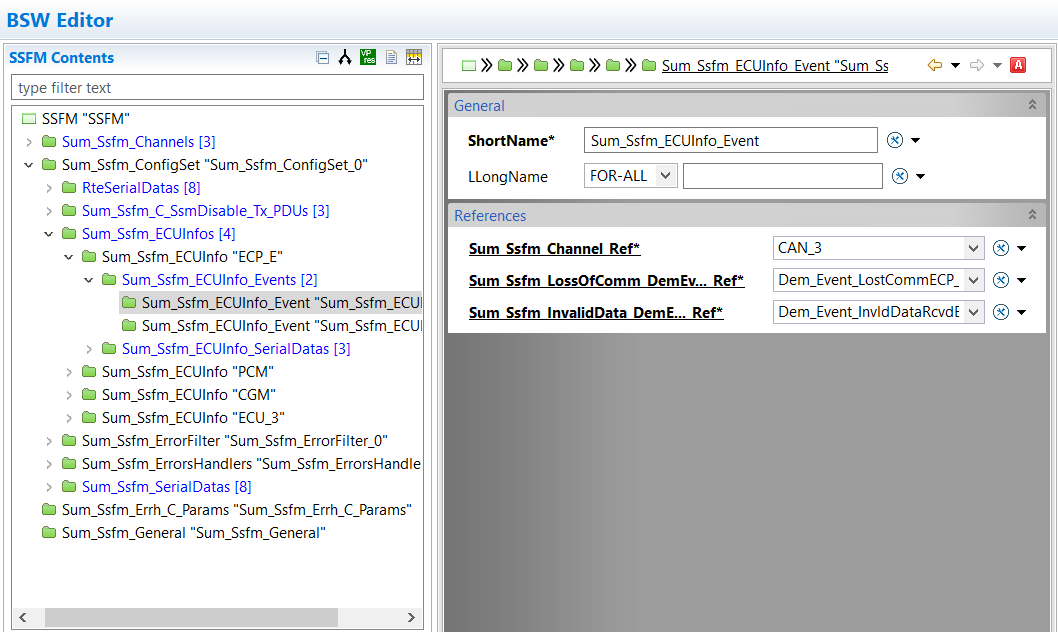
\includegraphics[width=0.7\textwidth]{images/ECUInfo_Events}
\end{center}

\paragraph{For LIN Communication}
\label{par:lininfogroup}
SUM\_LNM must be available beforehand, as SSFM requires the configuration in SUM\_LNM for getting LIN Responder information.
The user shall also create each instance of a LIN Responder referenced in the container \textbf{Sum\_Ssfm\_LINInfo} and configure the following steps:
\begin{enumerate}
	\item The container \textbf{Sum\_Ssfm\_LINInfo} contains references to a LIN Responder and an SSFM channel contained LIN SerialData.
	\item The container \textbf{Sum\_Ssfm\_LINInfo\_Event} contains references to the Dem event that will be used to signal invalid data events.
	\item The container \textbf{Sum\_Ssfm\_LINInfo\_SerialData} contains instances of SerialData that belong to the referenced LIN Responder.
\end{enumerate}
This configuration will enable the SSFM to set the events for Invalid Data DTCs for the SerialData associated with that LIN Responder.
\\\textbf{Note 1:} Support for multiple providers on a LIN device is not available.
\\\textbf{Note 2:} The SSFM channel referenced for a LIN Responder must be the same as the channel for each associated SerialData.

\begin{center}
	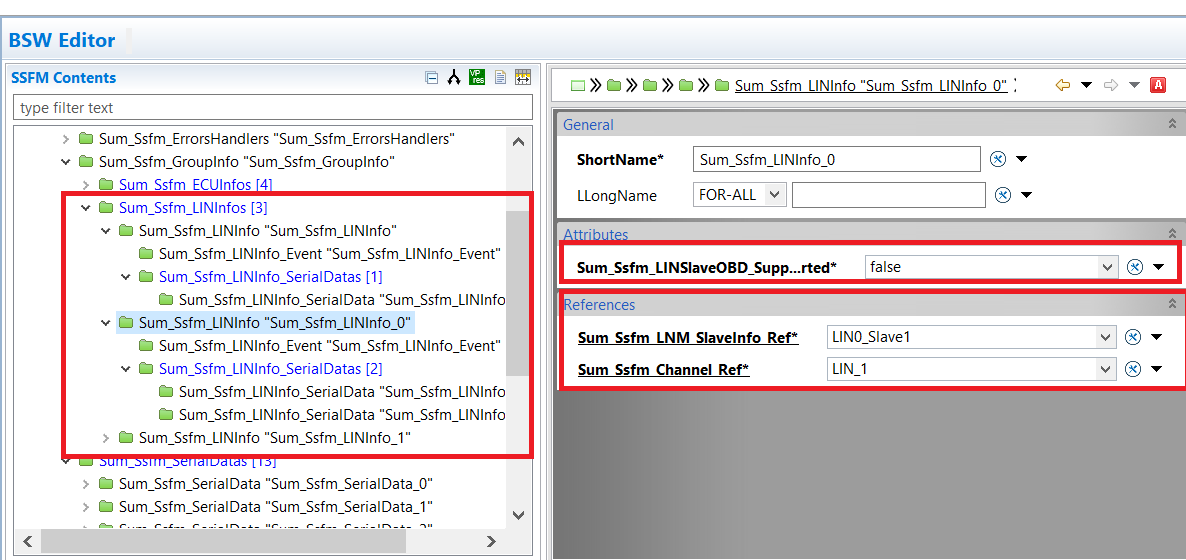
\includegraphics[width=0.7\textwidth]{images/LINInfo}
\end{center}

\begin{center}
	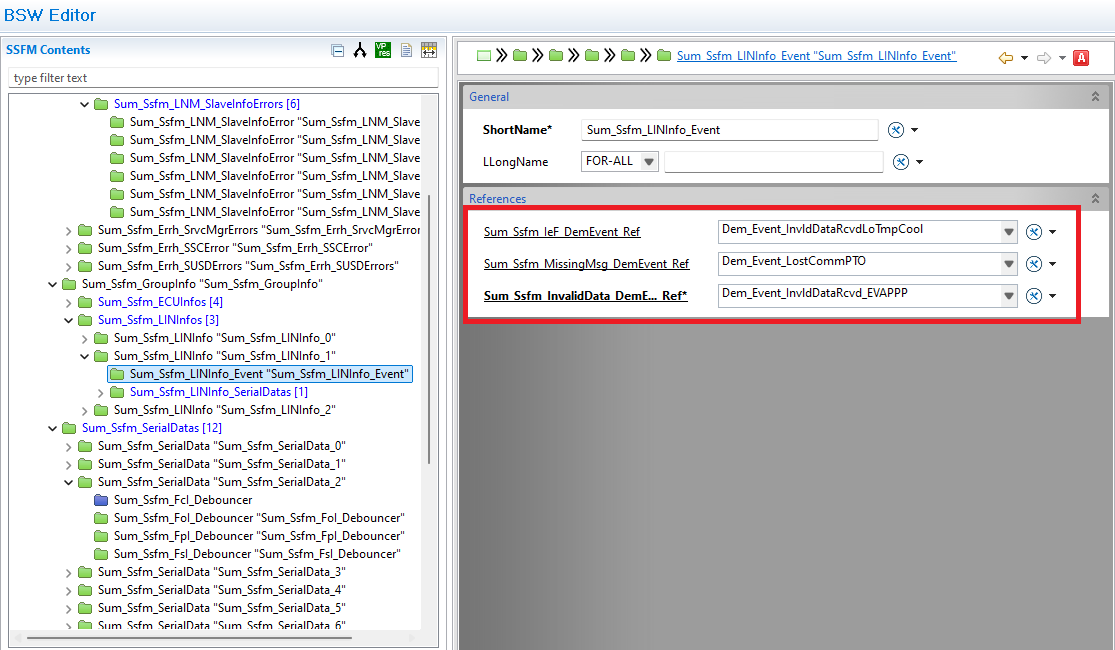
\includegraphics[width=0.7\textwidth]{images/LINInfo_Events}
\end{center}

\begin{center}
	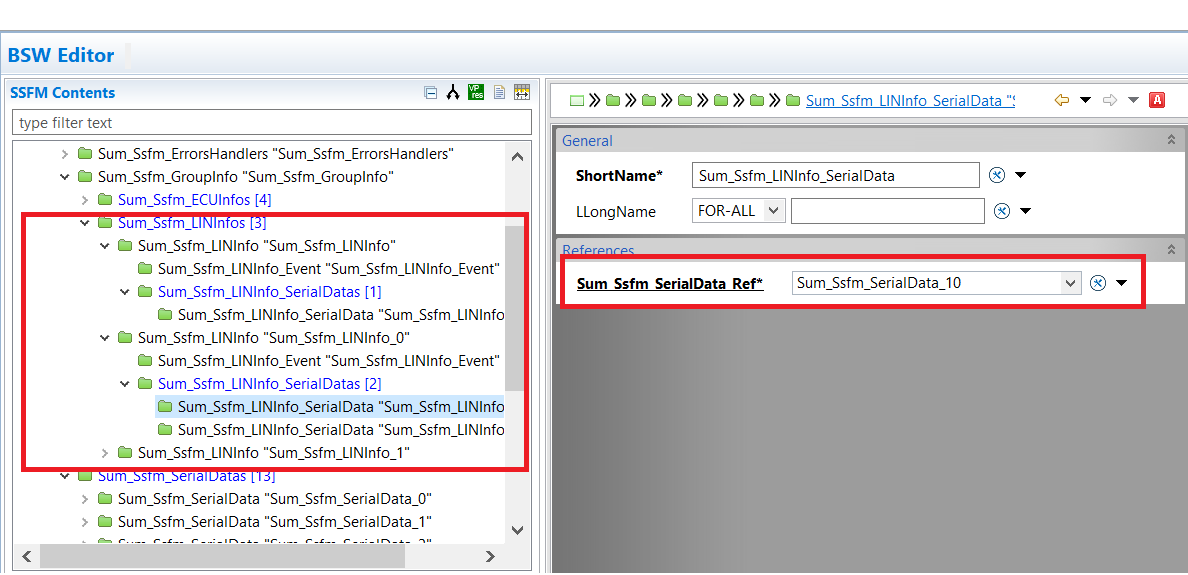
\includegraphics[width=0.7\textwidth]{images/LINInfo_SerialDatas}
\end{center}

\paragraph{Asking the Security Status Manager to reset the corresponding FcI interface}
To get notifications about the security status of a SerialData, the users should connect the corresponding PP\_SSFM\_SSM\_Sig\_<Signal\_Group\_Name>\_FcI to the port from which they read the SerialData security indication.
It is required to config the Sum\_Ssfm\_SecOCRxPdu\_Ref for the desired SerialData. 

\paragraph{Asking the Continuous Operation Status Manager to set the corresponding FoI interface according to the transformer error}
To get notifications about the continuous operation status of a SerialData, the users should connect the corresponding PP\_SSFM\_SSM\_Sig\_<Signal\_Group\_Name>\_FoI to the port from which they read the SerialData continuous operation indication.

\paragraph{Asking the Protection Status Manager to set the corresponding FpI interface state (for protected signals)}
To get notifications about the protection status of a SerialData, the users should connect the corresponding PP\_SSFM\_SSM\_Sig\_<Signal\_Group\_Name>\_FpI to the port from which they read the SerialData protection indication.

\paragraph{Asking the Safety Status Manager to update the corresponding FsI interface state (for protected or safety protected signals)}
To get notifications about the safety status of a SerialData, the users should connect the corresponding PP\_SSFM\_SSM\_Sig\_<Signal\_Group\_Name>\_FsI to the port from which they read the SerialData safety indication.

\paragraph{Asking the Single Port FxI Manager to update the FxI interface state}
To get notifications about the fault indication status of a SerialData, the users should connect the corresponding PP\_SSFM\_SSM\_Sig\_<Signal\_Group\_Name>\_FxI to the port from which they read the SerialData fault indication.
Note that this interface will be provided only if the \\ Sum\_Ssfm\_FxI\_FxFA\_SinglePortsSupport is enabled under the Sum\_Ssfm\_General. In this case, the previously mentioned FcI, FoI, FpI, and FsI interfaces will not be created.

\paragraph{Setting signal status availability of all SerialDatas}
To allow the Received SerialData Handler to set signal status availability when received for all SerialDatas.

\subsubsection{SSFM Security Status Manager}
\label{subsec:securitystatusmanager}

The Security Status Manager is responsible for the following tasks:

\begin{enumerate}
\item Resetting the FcI state to false whenever asked by the Received SerialData Handler or when it receives SECOC\_NO\_VERIFICATION error and the MAC Authentication is disabled.
\item Setting the FcI to true whenever it receives a MAC verification failure notification from SecOC (including when the MAC verification failure is SECOC\_NO\_VERIFICATION and the MAC Authentication is enabled).
\item Handling the FcI error status maturation, setting the corresponding Dem Event, and providing FcFA upon the DTC Confirm (TestFailed bit)
\end{enumerate}

\paragraph{Resetting the FcI state to false}
To allow the Security status Manager to reset the FcI state to false, the user should perform all the actions already highlighted in the paragraph above.

\paragraph{Setting the FcI state to true}
To allow the Security Status Manager to set the FcI interface to true, the user should include a callout named \textbf{SSFM\_Verification\_Status\_Callout} in the SecOCVerificationStatusCallout container.
To allow both actions, the user should connect RP\_SSFM\_SSM\_AuthenticationEnabled ports to SSC.

\paragraph{FcI Error maturation and FcFA}
To allow the Security Status Manager to handle the error maturation and setting the FcFA, the user shall config the \textbf{Sum\_Ssfm\_FcI\_Debouncer} sub-container for the desired SerialData.
The user shall also configure a \textbf{DemCallbackDTCStatusChanged} instance under the Dem General Configuration 
with a callback function named as \textbf{Ssfm\_Dem\_CB\_DTCStatusChanged} to enable the DTC setting feature.
To enable setting the Fault Active Status, it is necessary to connect the SPM\_GetDTCIdentifier interface.
\\\textbf{Note 1:} Please note that the \textbf{Sum\_Ssfm\_EventFilter\_Ref} can point to the same reference among different Fault Indications, assuming that they use the same debouncing algorithm. 
\\\textbf{Note 2:} The Security Status Manager is not applicable for LIN.

\subsubsection{SSFM Continuous Operation Status Manager}
\label{subsec:continuousoperationstatusmanager}

The Continuous Operation Status Manager is responsible for the following tasks:

\begin{enumerate}
\item Setting the FoI state based on the given transformer error whenever asked by the Received SerialData Handler
\item Handling the FoI error status maturation, setting the corresponding Dem Event, and providing FoFA upon the DTC Confirm (TestFailed bit)
\end{enumerate}

\paragraph{Setting the FoI state based on the given transformer error whenever asked by the Received SerialData Handler}
To allow the Continuous Operation Status Manager to set or reset the FoI state, the user should perform all the actions already highlighted in the paragraph above.

\paragraph{FoI Error maturation and FoFA}
To allow the Continuous Operation Status Manager to handle the error maturation and setting the FoFA, the user shall config the \textbf{Sum\_Ssfm\_FoI\_Debouncer} sub-container for the desired SerialData.
The user shall also configure a \textbf{DemCallbackDTCStatusChanged} instance under the Dem General Configuration 
with a callback function named as \textbf{Ssfm\_Dem\_CB\_DTCStatusChanged} to enable the DTC setting feature.
To enable setting the Fault Active Status, it is necessary to connect the SPM\_GetDTCIdentifier interface.
\\\textbf{Note 1:} Please note that the \textbf{Sum\_Ssfm\_EventFilter\_Ref} can point to the same reference among different Fault Indications, assuming that they use the same debouncing algorithm. 

\subsubsection{SSFM Protection Status Manager}
\label{subsec:protectionstatusmanager}

The Protection Status Manager is responsible for the following tasks:

\begin{enumerate}
\item Setting the FpI state based on the given transformer error whenever asked by the Received SerialData Handler
\item Setting the FpI state based on the given desired state whenever asked by other modules
\item Handling the FpI error status maturation, setting the corresponding Dem Event, and providing FpFA upon the DTC Confirm (TestFailed bit) 
\end{enumerate}

\paragraph{Setting the FpI state based on the given transformer error whenever asked by the Received SerialData Handler}
To allow the Protection Status Manager to set or reset the FpI state, the user should perform all the actions already highlighted in the paragraph above.

\paragraph{Setting the FpI state based on the given desired state whenever asked by other modules}
To allow the Protection Status Manager to set or reset the FpI state, the user should perform all the actions already highlighted in the paragraph above.

\paragraph{FpI Error maturation and FpFA}
To allow the Protection Status Manager to handle the error maturation and setting the FpFA, the user shall config the \textbf{Sum\_Ssfm\_FpI\_Debouncer} sub-container for the desired SerialData.
The user shall also configure a \textbf{DemCallbackDTCStatusChanged} instance under the Dem General Configuration 
with a callback function named as \textbf{Ssfm\_Dem\_CB\_DTCStatusChanged} to enable the DTC setting feature.
To enable setting the Fault Active Status, it is necessary to connect the SPM\_GetDTCIdentifier interface.
\\\textbf{Note 1:} Please note that the \textbf{Sum\_Ssfm\_EventFilter\_Ref} can point to the same reference among different Fault Indications, assuming that they use the same debouncing algorithm. 

\subsubsection{SSFM Safety Status Manager}
\label{subsec:safetystatusmanager}

The Safety Status Manager is responsible for the following tasks:

\begin{enumerate}
\item Updating the FsI state whenever asked by other modules
\item Handling the FsI error status maturation, setting the corresponding Dem Event, and providing FsFA upon the DTC Confirm (TestFailed bit)
\end{enumerate}

\paragraph{Updating the FsI state whenever asked by other modules}
To allow the Safety Status Manager to set or reset the FsI state, the user should perform all the actions already highlighted in the paragraph above.

\paragraph{FsI Error maturation and FsFA}
To allow the Saftey Status Manager to handle the error maturation and setting the FsFA, the user shall config the \textbf{Sum\_Ssfm\_FsI\_Debouncer} sub-container for the desired SerialData.
The user shall also configure a \textbf{DemCallbackDTCStatusChanged} instance under the Dem General Configuration 
with a callback function named as \textbf{Ssfm\_Dem\_CB\_DTCStatusChanged} to enable the DTC setting feature.
To enable setting the Fault Active Status, it is necessary to connect the SPM\_GetDTCIdentifier interface.
\\\textbf{Note 1:} Please note that the \textbf{Sum\_Ssfm\_EventFilter\_Ref} can point to the same reference among different Fault Indications, assuming that they use the same debouncing algorithm. 

\subsubsection{SSFM Single Port FxI Manager}
\label{subsec:singleportFxI}

The Single Port FxI Manager is responsible for updating the FxI state whenever asked by other modules. 
To enable the single port FxI/FxFA feature in SSFM it is required to set to True the parameter \\ (Sum\_Ssfm\_FxI\_FxFA\_SinglePortsSupport).
Having the mentioned parameter as True, causes the SSFM to provide a single FxI port instead of the four FcI, FoI, FpI, and FsI and a 
single FxFA port instead of the four FcFA, FoFA, FpFA, and FsFA.

\subsubsection{SSFM multiple proivder serial data}
\label{subsec:multipleprovider}
The SSFM uses the SSM\_C\_<PDU name>\_IsReceivedFrom\_<ECU name> calibration parameter to check the current provider of a given PDU
at the time of initialization. Later, all the invalid data events will be set against the actual provider.

\subsection{SSFM Message Info Handler}
\label{sec:ssfmmessageinfohandler}
\subsubsection{SSFM Disable PDU}
\label{subsec:disablepdu}
The SSFM is capable to disable, at init time, some TX PDU configured by the user. To do that you need to create the container Sum\_Ssfm\_C\_SsmDisable\_Tx\_PDU for each PDU that you want to disable 
(please, remember to create a container for each protected Tx PDU, even if the PDU is always enabled).
Two ports and a calibration parameter (SSM\_C\_Disable\_<Pduname>) will be created for each PDU.

\begin{center}
	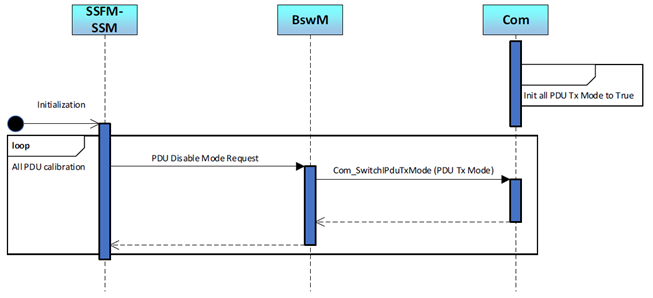
\includegraphics[width=0.7\textwidth]{images/disablepdu}
\end{center}

\subsubsection{SUM\_BswM\_DisablePdu}
\label{subsec:ssfmdisablepdu}
The P-Port related to the interface \textbf{SUM\_BswM\_DisablePdu} shall be connected to the relative one of the BswM. It enables the SSFM\_SSM to disable the Tx PDU.
To create it, in the BswM you need to configure a \textbf{BswMModeRequestPort} that is referencing this interface.
You also need to configure an action of type \textbf{BswMSwitchIPduMode} that references the PDU that the P-Port is indicating in its name. 
Through the Conditions, Expressions and Rules, when the P-Port is writing, the corresponding BswM Action of PDU disable is invoked.

\subsubsection{SUM\_C\_Disable\_Tx\_<n>}
The P-Port related to the interface \textbf{SUM\_C\_Disable\_Tx\_<n>} are generated for all the PDUs that could be disabled by the relative calibration parameter. Those ports shall be
connected to SUM\_SSC and SUM\_PNC. The SSC will be connected and use only the ports related to protected PDU, PNC instead will use all of them.

\subsubsection{PN\_DTC\_Allowed<n>}
\label{subsec:ssfmpndtcallowed}
The R-Port related to the interface \textbf{PN\_DTC\_Allowed<n>} shall be connected to the relative one of the PNC. It enables the SSFM\_SSM to get notified of a status
change in any partial network relatively to the settability of DTCs.

\subsubsection{Signal\_Status\_Availability}
\label{subsec:ssfmsigstatusavail}
The Message Information Handler is responsible for the following tasks:
\begin{enumerate}
    \item Check for the relevant Partial Networks are active of a SerialData.
    \item Check for Disable Normal Communication of a SerialData.
    \item Check for Disable PDU of a SerialData.
    \item Set the supervision status of a SerialData.
    \item Check for SecOC verification status of a SerialData.
\end{enumerate}

\subsection{Signal Status Availability Manager}
\label{subsec:ssfmsigstsmanager}
\subsubsection{CANETH\_Signal\_Status\_Manager}
The CAN/ETH Signal Status Availability Manager shall set the signal availability of all signals upon any change in availability conditions.

\paragraph{Checking at least a relevant Partial Network is active of a SerialData}
To get the status if there is at least one Partial Network is active via reading configured R-Port interfaces \textbf{PNC\_ActiveRxPDUEnable<SerialData\_Name>}. 

Note: A SerialData can pariticipate to multiple partial networks.

\paragraph{Checking the service activation status}
Whenever a SerialData is associated with the service-based traffic the activation status of the SerialData, received by SPM, will be used instead of the Partial Network activation status.
To this end, the user shall configure the parameter \textbf{Sum\_Ssfm\_SDService\_Ref} pointing to the corresponding client or server service.

Please note that a SerialData must not have references to both Partial Network and SD Client$\backslash$Server Service.

\paragraph{Checking normal communication is disable of a SerialData}
To get the status if normal communication is disable via reading configured R-Port interface \newline
\textbf{DIAG\_DisableNormalComm<channel>}.

\paragraph{Checking the disable PDU of a SerialData} 
To get the status if PDU for a particular SerialData is disable via reading configured calibration parameter (SSM\_C\_Disable\_<Pduname>).

\paragraph{Setting the supervision status for a SerialData} 
To set the signal supervision status through data received event of a runnable and Com callback timeout configured for the SerialData.

\paragraph{Checking SecOC verification status of a authenticated SerialData} 
To get the status if SecOC verification status is failed by getting FcI interface.

\paragraph{Checking Node Status or Lost Communication Status of the provider controller}
To get the Node Status of the current provider controller it is necessary to connect the \textbf{SSFM\_IF\_NodeStsECU\_LcFA} interface from the Gateway controller to SSFM.

\paragraph{Non-Discoverable SOME/IP Services}
SerialDatas with \textbf{Sum\_Ssfm\_IsNonDiscoverable} set to TRUE represent signal-based SOME/IP services without Service Discovery. These services:
\begin{itemize}
    \item Are always Available (initialized once, state machine bypassed)
    \item Bypass Partial Network precondition checks in FxI debouncing
    \item Are excluded from LoC monitoring (LostCommInfo = NULL\_PTR)
    \item Support only FcI and FsI fault indications
\end{itemize}
Configuration: Set \textbf{Sum\_Ssfm\_IsNonDiscoverable} to TRUE. Do NOT configure PN references, LoC parameters, or fault detection usage.

Below there is a sample configuration:

\begin{figure}[H]
	\centering
	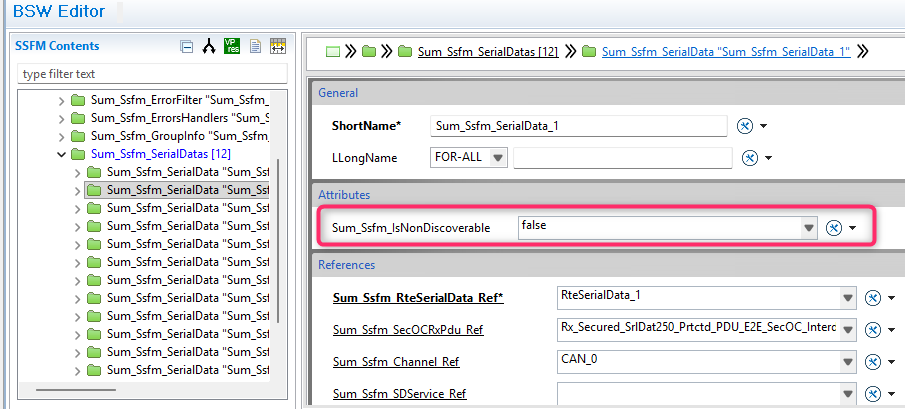
\includegraphics[scale=0.50]{images/nondiscoverable_config_example.png}
	\caption{Non-discoverable SOME/IP service configuration example}
	\label{fig:nondiscoverable_config}
\end{figure}
It is necessary to configure a few attributes and references:
\begin{enumerate}
    \item \textbf{Sum\_Ssfm\_Channel\_Ref}: reference to Sum\_Ssfm\_Channel
    \item \textbf{Sum\_Ssfm\_Channel\_ID\_Ref}: reference to the ComM Channel for Ethernet/CAN, LIN SerialData.
    \item \textbf{Sum\_Ssfm\_C\_SsmDisable\_Rx\_PDURef}: to RX signal for which to create calibration parameter to enable/disable it.
    \item \textbf{Sum\_Ssfm\_Partial\_Network\_Ref} or \textbf{Sum\_Ssfm\_SDService\_Ref}: reference to partial networks SerialData participated or to sd client$\backslash$server service related. Note that 
    this is an exclusive "or". A SerialData shall not have references to both.
\end{enumerate}

\subsection{Loss of Communication - Node Status Manager}
\label{subsec:NodeStatusManager}

The Node Status Manager is responsible for monitoring the loss of communication with different controllers, whether they are communicating directly or through the gateway module.
To enable the functionality the ECUInfo entities should be configured correctly in the \textbf{Sum\_Ssfm\_ConfigSet}.
For each ECU, the related SerialDatas should be added as a \textbf{Sum\_Ssfm\_ECUInfo\_SerialData}. 
Then, the routing method of each SerialData should also be defined using the parameter \\ \textbf{Sum\_Ssfm\_RoutingMethod}.
Moreover, when the integrator is defining the Central Gateway Module, the \textbf{Sum\_Ssfm\_IsGateway} should be set to true for the ECUInfo instance of the CGM ECU.

\textbf{Note}: Non-discoverable SOME/IP SerialDatas (\textbf{Sum\_Ssfm\_IsNonDiscoverable} = TRUE) are automatically excluded from LoC monitoring and should not be added to ECUInfo fault/recovery lists.
If the current ECU is the gateway it is necessary to set the parameter \textbf{Sum\_Ssfm\_IsThisECUGateway} under the \textbf{Sum\_Ssfm\_General} container.
To properly update the status of DTCs reporting the loss of communication with a node for service-based and signal-based traffic, two sets of parameters should be configured:
\begin{itemize}
	\item for each possible target device, a reference to a configured SPM Target Device should be set in 
			the \\ \textbf{Sum\_Ssfm\_TrgDvcInfo} under \textbf{Sum\_Ssfm\_GroupInfo}.
	      	This will let the SSFM forward information on the status of Loss Of Communication events for 
			service-based communication from the SPM to the Dem.
	\item for each ECUInfo entity, a \textbf{Sum\_Ssfm\_ECUInfo\_Event} sub container shall be 
			configured for each SSFM channel referenced by SerialDatas configured by the ECUInfo.
	      	It contains a reference to the Dem event to be used for signaling loss of communication events 
		  	for the target controller.
	      	This will let the SSFM set events for Loss Of Communication DTCs for signal-based communication.
			Please note that \textbf{Sum\_Ssfm\_ECUInfo\_Event} shall be only defined for the channels used by signal based serial data. 
			If a channel is only used by service based serial data, there is no need to create this sub-container.
\end{itemize}

Given an ECU, all the SerialDatas that are communicating with the current ECU using a Direct or PDURouted routing can practically be used for monitoring loss of communication. 
In this case, each SerialData can be either be used for "fault and recovery" detection or "recovery only" detection.
In this sense, the list of fault detection SerialDatas will be a subset of the recovery detection list.
In order to use a SerialData for fault detection the parameter \textbf{Sum\_Ssfm\_FaultDetectionUsage} should be set to \textbf{FaultAndRecovery}.
This participation in fault detection has to be set using parameter \textbf{Sum\_Ssfm\_FaultDetectionUsage} in \textbf{Sum\_Ssfm\_ECUInfo\_SerialData}.

Please note that for the service based traffic cannot be added as a \textbf{Sum\_Ssfm\_ECUInfo\_SerialData}. The service based traffic will be provider instead by 
one of the configured \textbf{Sum\_Ssfm\_TrgDvcInfo}, pointing to a SPM target device. All these target devices could be a possible provider for all service-based serial datas.
The actual provider will be resolved at runtime thanks to the APIs from SD and SPM. In this case, all the services provided by a provider will be assumed as "fault and recovery" serial data.
To be more precise, the service-based target devices will not have any "recovery only" serial data.  

Whenever the current ECU is the CGM, the SSFM is responsible also for providing the NodeStsECU interface to provide the loss of comm for the controllers that communicate with each other through the CGM.
CGM looks into the channels used by ECUs to communicate with it. If there is only one channel used to communicate, then CGM provides the interface with \code{NodeStsECU_<ecu_name>} format. 
Instead, if multiple channels are being used, the provide interface follows the format \\ \code{NodeStsECU_<ecu_name>_CAN_<channel_id>}. 

Every ECUInfo may be related to different controllers. For instance, an ECU may provide two or more different controllers like ECU\_X\_CAN\_Y.
These controllers might be either service based or signal based. While a single controller cannot be service and signal based at the same time,
an ECU may have different controllers of different types. 
While it is mandatory to configure \textbf{Sum\_Ssfm\_LossCommID} for ECUInfos with at least one signal based controller,
the parameter should not be configured if the ECUInfo does not provide any signal based controllers.
Please note that \textbf{Sum\_Ssfm\_LossCommID} should be unique for all the instances of \\ \textbf{Sum\_Ssfm\_ECUInfo}.

It is necessary for the user to configure the channel reference of each SerialData correctly according to the routing method as follows:

\begin{itemize}
    \item Direct Routed and Signal Routed SerialDatas: The channel reference should be the channel on which the current ECU receives data from. In case of signal routed SerialDatas the channel will be the one that the CGM communicates with the current ECU on it.
    \item PDU Routed: The channel reference should be the channel on which the transmitter ECU communicates with the CGM. Since this channel is out of the scope of the current ECU, the configured SSFM Channel may not have a reference to a ComMChannel instance. 
\end{itemize}

Moreover, the SSFM channels should be configured with a name like CAN\_<n> or ETH\_<n> since the Node Status Manager will use the name in the ports communicating the Node Status.

\subsubsection{Service Based Traffic}
\label{subsec:LossOfCommService}
Regarding the service-based traffic, the user can also monitor the loss of function by configuring the provider ECUInfo and the corresponding ECUInfo\_SerialData.
The fault and recovery logic will act the same as the non-service-based traffic. The user shall configure the \\ \textbf{Sum\_Ssfm\_SpmTargetDevice\_Ref}
for the ECUInfo which has a service-based controller. Please note that a controller should either provide service-based or non-service-based traffic. This is an exclusive "or".


\subsubsection{Node Loss Error Manager}
\label{subsec:NodeLossErrorManager}

The Node Loss Error Manager is responsible for monitoring the ECU node loss error maturation. To enable the functionality the ECUInfo entities should be configured correctly mentioned in ~\ref{subsec:NodeStatusManager}. 
The user shall configure \textbf{Sum\_Ssfm\_Errh\_C\_DTCProcess\_SsmNodeLoss} in \textbf{Sum\_Ssfm\_ECUInfo} for each ECU to control whether to process DTC for SSM Node Loss Error. 

\begin{figure}[H]
	\centering
	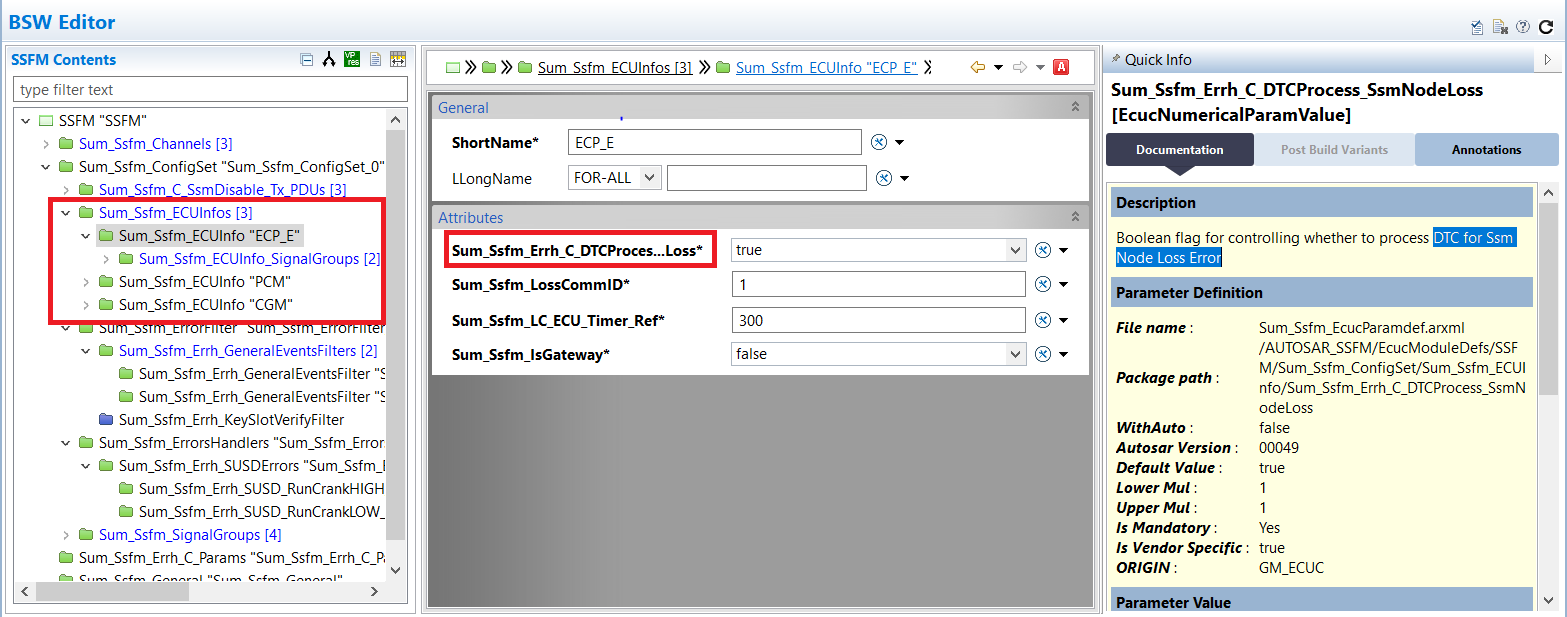
\includegraphics[scale=0.40]{images/NodeLossManager.PNG}
\end{figure}

The user shall configure \textbf{Sum\_Ssfm\_LC\_ECU\_Timer\_Ref} in \textbf{Sum\_Ssfm\_ECUInfo} for each ECU to configure ECU Node Loss debouncer timer in millisecond. 

\begin{figure}[H]
	\centering
	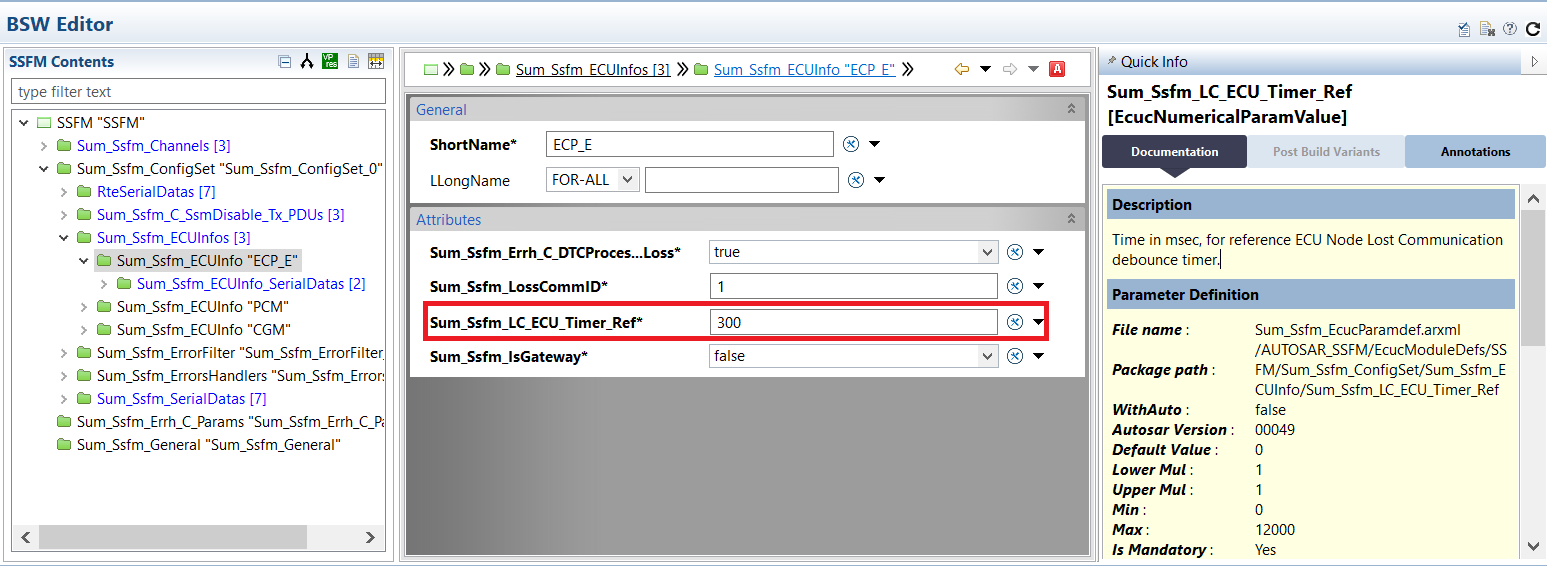
\includegraphics[scale=0.40]{images/NodeLossLCTimer.PNG}
\end{figure}

\paragraph{Setting the runnable periodicity parameter \newline Sum\_Ssfm\_NodeLossError\_RunnablePeriodicity}
The periodicity parameter sets the period in which the runnable responsible for handling the Node Loss Error is being called.
In order to have no drift and no missed verification, make sure that the parameter value is divisible by the Sum\_Ssfm\_LC\_ECU\_Timer\_Ref and the corresponding calibration parameter for all the configured ECUInfo.
The Sums will check for this compatibility at generation time using the default value set for the calibration parameter. However, it's upon user to make sure that the periodicity remains divisible by the calibration values during the runtime.


\subsubsection{Usage of CAN\_BUS\_OFF\_DTC for Loss of communication}
\label{subsec:UsageOfCanBusOffDtcInLossOfComm}

For all configured containers \textbf{Sum\_Ssfm\_Channel} the calibration parameter \newline \textbf{Sum\_Ssfm\_Ssm\_C\_UsageOfCanBusOffDTC} has to be configured. 
This has to be set to false if the channel is not a communication bus of type CAN. 
In case the bus is of type CAN and the CAN\_BUS\_OFF\newline \_DTC is used to set the Loss of communication the parameter should be set to true. 

\begin{figure}[H]
	\centering
	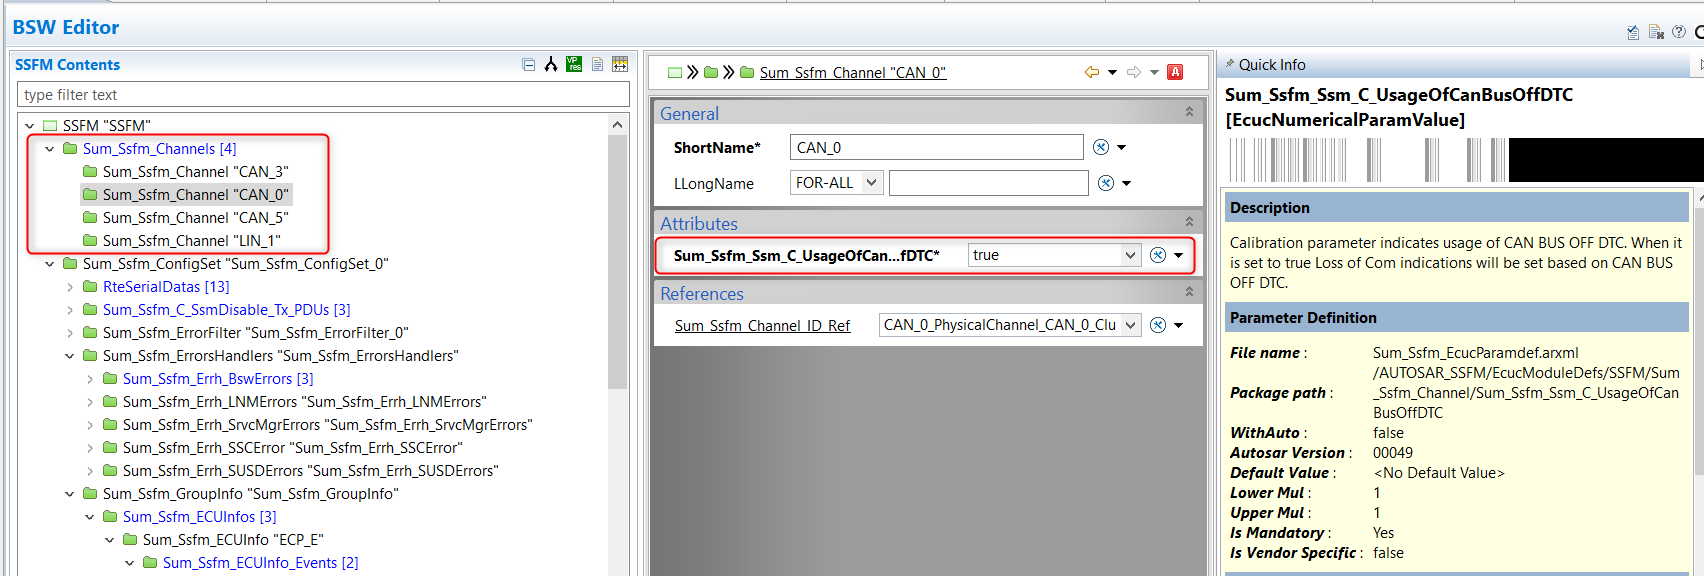
\includegraphics[scale=0.40]{images/UsageOfCanBusOffDtcInLossOfCommunication.PNG}
\end{figure}

\subsection{DTC Enable Criteria}
\label{subsec:DTCEnableCriteria}

There are two flags which check two conditions:
\begin{itemize}
    \item \code{Sum_Ssfm_ResetPowerUpRecoveryTimer}
	\item \code{Sum_Ssfm_BatteryVoltageRecoveryTimer}
\end{itemize}

\subsubsection{Sum\_Ssfm\_ResetPowerUpRecoveryTimer}
The R-Port related to the interface \textbf{BatteryVoltageRangeMinToMax} shall be connected to \\SUM\_SUSD. In Sum\_SUSD the container SUSD\_Battery\_Voltage\_Supported shall be enabled and the minimum and maximum voltage shall be defined. 
SUM\_SSFM shall receive battery voltage level using this port.


\subsection{SSFM ERRH DTC U19A3 57 Handler}
\label{subsec:SSFMERRHDTCU19A357Handler}
The EERH DTC U19A3 57 Handler is responsible to aggregate the status of U19A3 57 failures. 
To enable the execution of the ERRH DTC U19A3 57 Handler, the user must:
\begin{itemize} 
	\item configure the SSC module, setting the parameter InVehicleMessageAuthentictnSupprted to a non-zero value (typically 1);
	\item set the parameter Sum\_Ssfm\_Errh\_CodeGen\_Enabled, present in Sum\_Ssfm\_Errh\_U19A3\_57\\\_InvIncCfg in SSFM module, to true.
\end{itemize}
It should be noted that the parameter Sum\_Ssfm\_Errh\_CodeGen\_Enabled can be configured as true or false; by setting it to false, the SSFM module can be used regardless of the presence of SSC module.


\subsubsection{DTC  U19A3 57}
The DTC  U19A3 57 indicates the failure regarding the Control Module-Invalid/Incompatible Configuration.

\paragraph{Sum\_Ssfm\_Errh\_C\_DTC\_U19A3\_57\_InvIncCfg}
In order to enable the aggregation of DTC U19A3 57, the designated calibration parameter should be set to \code{true}.

\paragraph{BatteryVoltageRangeMinToMax interface}
The BatteryVoltageRangeMinToMax interface should be properly connected as described in \ref{subsec:DTCEnableCriteria}. In case of the OBD support the
functionality of U19A3 57 56 will be enabled if the battery voltage is not less than the normal range. On the other hand, in case of no OBD support, the
battery voltage should be explicitly in normal range to have the U19A3 57 functionality enabled.

\paragraph{SSC\_ERRH\_DTC\_U19A3\_57\_Status}
The SSFM reads the status of DTC U19A3 57 through the designated interface provided by SUM\_SSC. Therefore, the SSC\_ERRH\_DTC\_U19A3\_57\_Status should 
be properly connected to the SSFM.


\subsection{SSFM ERRH DTC U19A3 Handler}
\label{subsec:SSFMERRHDTCU19A3Handler}
The ERRH DTC U19A3 92 Handler is responsible for handling the U19A3 92 DTC and reporting its status to Dem.

\subsubsection{DTC U19A3 92}

The DTC U19A3 92 indicates the failure regarding the Security Peripheral-Performance/Incorrect Operation.
To enable the execution of the ERRH DTC U19A3 92 Handler, the user must:
\begin{itemize} 
	\item configure the SSC module, setting the parameter intgrtedSecrtyPeriphrlKeyStrgPresent to true;
	\item set the parameter Sum\_Ssfm\_Errh\_CodeGen\_Enabled, present in Sum\_Ssfm\_Errh\_U19A3\_92\\\_SecPer\_PerIncOp in SSFM module, to true.
\end{itemize}
It should be noted that the parameter Sum\_Ssfm\_Errh\_CodeGen\_Enabled can be configured as true or false; by setting it to false, the SSFM module can be used regardless of the presence of SSC module.

\paragraph{Sum\_Ssfm\_Errh\_C\_DTC\_U19A3\_92\_SecPer\_PerIncOp}
In order to enable the DTC U19A3 92, the designated calibration parameter should be set to \code{true}.

\paragraph{BatteryVoltageRangeMinToMax interface}
The BatteryVoltageRangeMinToMax interface should be properly connected as described in \ref{subsec:DTCEnableCriteria}. In case of the OBD support the
functionality of U19A3 92 will be enabled if the battery voltage is not less than the normal range. On the other hand, in case of no OBD support, the
battery voltage should be explicitly in normal range to have the U19A3 92 functionality enabled.

\paragraph{BswM configuration}
The SSFM component includes the RPort RP\_BswM\_SSFM\_SecPError for receiving the HSM error notification from BswM.
For the correct error code reporting, SSFM assumes that BswM configuration includes the definition of:

\begin{itemize}
	\item a Mode Switch Port to be connected to RP\_BswM\_SSFM\_SecPError;
	\item a Mode Request Port to receive mode change requests from Cry module;
	\item a Rule for each mode change notification to SSFM.
\end{itemize}

\subsection{DTC U19A3 54}
\label{subsubsec:SSFMERRHDTCU19A354Handler}
The DTC U19A3 54 indicates the failure regarding the Security Peripheral-Missing Setup/Learn.

\paragraph{Sum\_Ssfm\_Errh\_C\_DTC\_U19A3\_54\_SecPer\_MissSetup }
In order to enable the DTC U19A3 54, the designated calibration parameter should be set to \code{true}.

\paragraph{BatteryVoltageRangeMinToMax interface}
The BatteryVoltageRangeMinToMax interface should be properly connected as described in \ref{subsec:DTCEnableCriteria}. In case of the OBD support the
functionality of U19A3 54 will be enabled if the battery voltage is not less than the normal range. On the other hand, in case of no OBD support, the
battery voltage should be explicitly in normal range to have the U19A3 54 functionality enabled.

\paragraph{SSC\_ERRH\_DTC\_U19A3\_54\_Status interface}
The SSFM component includes the RPort RP\_SSC\_ERRH\_DTC\_U19A3\_54\_Status for receiving the DTC 19A3 54 error notification from SSC. 

\begin{figure}[H]
	\centering
	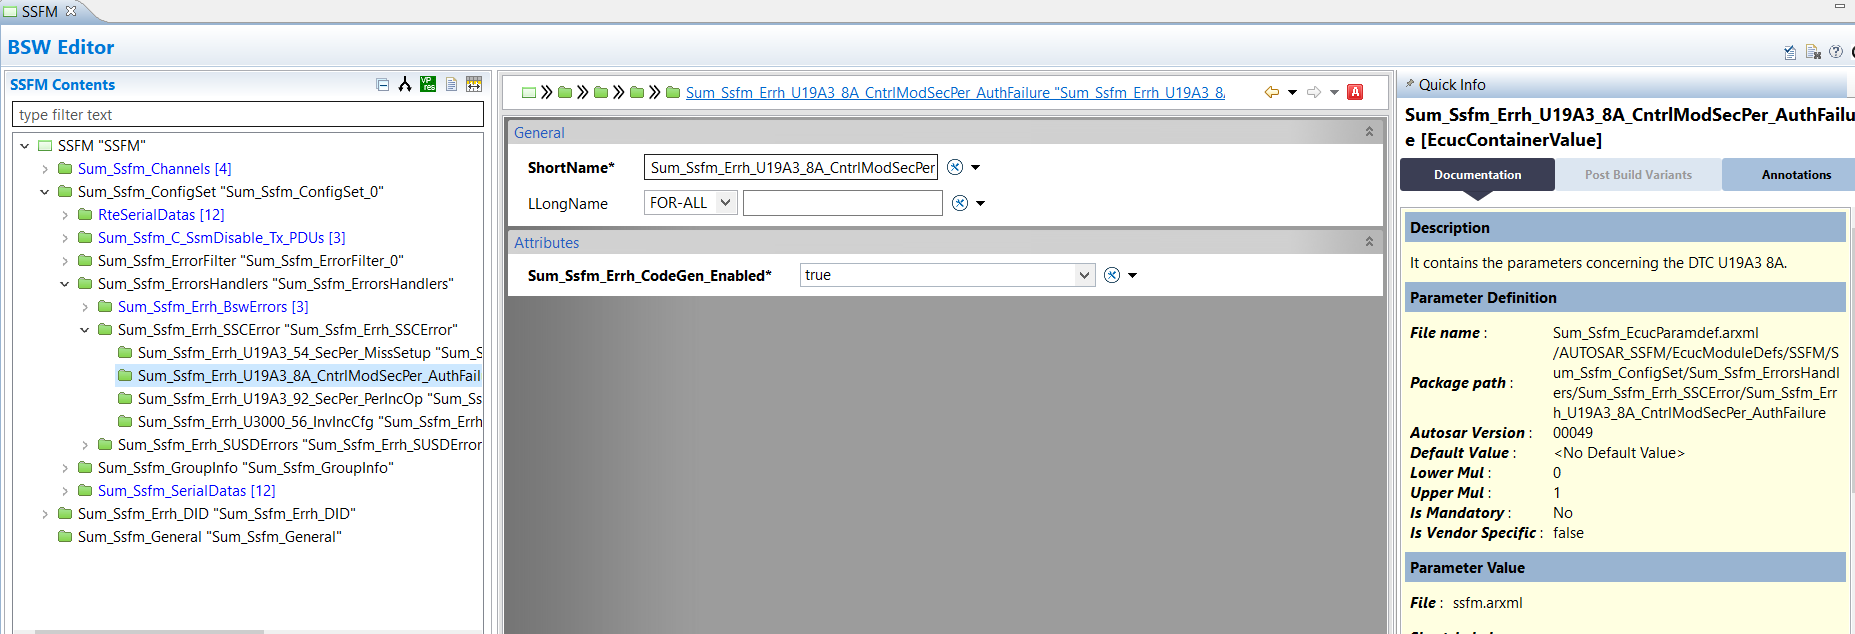
\includegraphics[scale=0.40]{images/Ssfm_Errh_SSCError.PNG}
\end{figure}

\subsection{DTC U19A6 54}
\label{subsec:SSFMERRHDTCU19A54AHandler}

The DTC U19A6 54 indicates the failure regarding the Service Discovery Failure- Missing Setup/Learn.

\paragraph{Sum\_Ssfm\_Errh\_C\_DTC\_U19A6\_54\_MissSetup }
In order to enable the DTC U19A6 54, the designated calibration parameter should be set to \code{true}.

\paragraph{BatteryVoltageRangeMinToMax interface}
The BatteryVoltageRangeMinToMax interface should be properly connected as described in \ref{subsec:DTCEnableCriteria}. In case of the OBD support the
functionality of U19A6 54 will be enabled if the battery voltage is not less than the normal range. On the other hand, in case of no OBD support, the
battery voltage should be explicitly in normal range to have the U19A6 54 functionality enabled.

\paragraph{DIAG\_GetMEC interface}
The DIAG\_GetMEC interface should be connected in order to support the DTC U19A6 54. The MEC value will be received through this interface.

\subsection{DTC U19A6 87}
\label{subsec:SSFMERRHDTCU19A687Handler}

The DTC U19A6 87 indicates the failure regarding the Service Discovery - Missing Message.

\paragraph{Sum\_Ssfm\_Errh\_C\_DTC\_U19A6\_87\_MissingMessage }
In order to enable the DTC U19A6 87, the designated calibration parameter should be set to \code{true}.

\paragraph{BatteryVoltageRangeMinToMax interface}
The BatteryVoltageRangeMinToMax interface should be properly connected as described in \ref{subsec:DTCEnableCriteria}. In case of the OBD support the
functionality of U19A6 87 will be enabled if the battery voltage is not less than the normal range. On the other hand, in case of no OBD support, the
battery voltage should be explicitly in normal range to have the U19A6 87 functionality enabled.

\paragraph{SrvcMgr\_SSFM\_LearningTableStatus}
The SrvcMgr\_SSFM\_LearningTableStatus interface should be connected in order to support the DTC U19A6 87. The LearningTableState value will be received through this interface.

\subsection{DTC U19A6 57}
\label{subsec:U19A657Handler}

The primary purpose of DTC U19A6 57 is to serve as an indicator to know when DID E0CE should be read for diagnostic information about failed service acknowledgments.

It should be noted that the parameter Sum\_Ssfm\_Errh\_U19A6\_57\_DTCProcess can be configured as true or false; by setting it to false, the SSFM module will not propagate this DTC.

\paragraph{Sum\_Ssfm\_Errh\_U19A6\_57\_DTCProcess} 
In order to enable the DTC U19A6 57, the designated calibration parameter should be set to \code{true}.

\paragraph{Sum\_Ssfm\_Errh\_SrvcMgr\_U19A6\_57\_Filter\_Ref}
Setting the reference to event filter for U19A6\_57 error.
To get the reference to the general event filter, the user should configure the Sum\_Ssfm\_GeneralEventFilter used for U19A6\_57 as the example image below.

\begin{figure}[H]
	\centering
	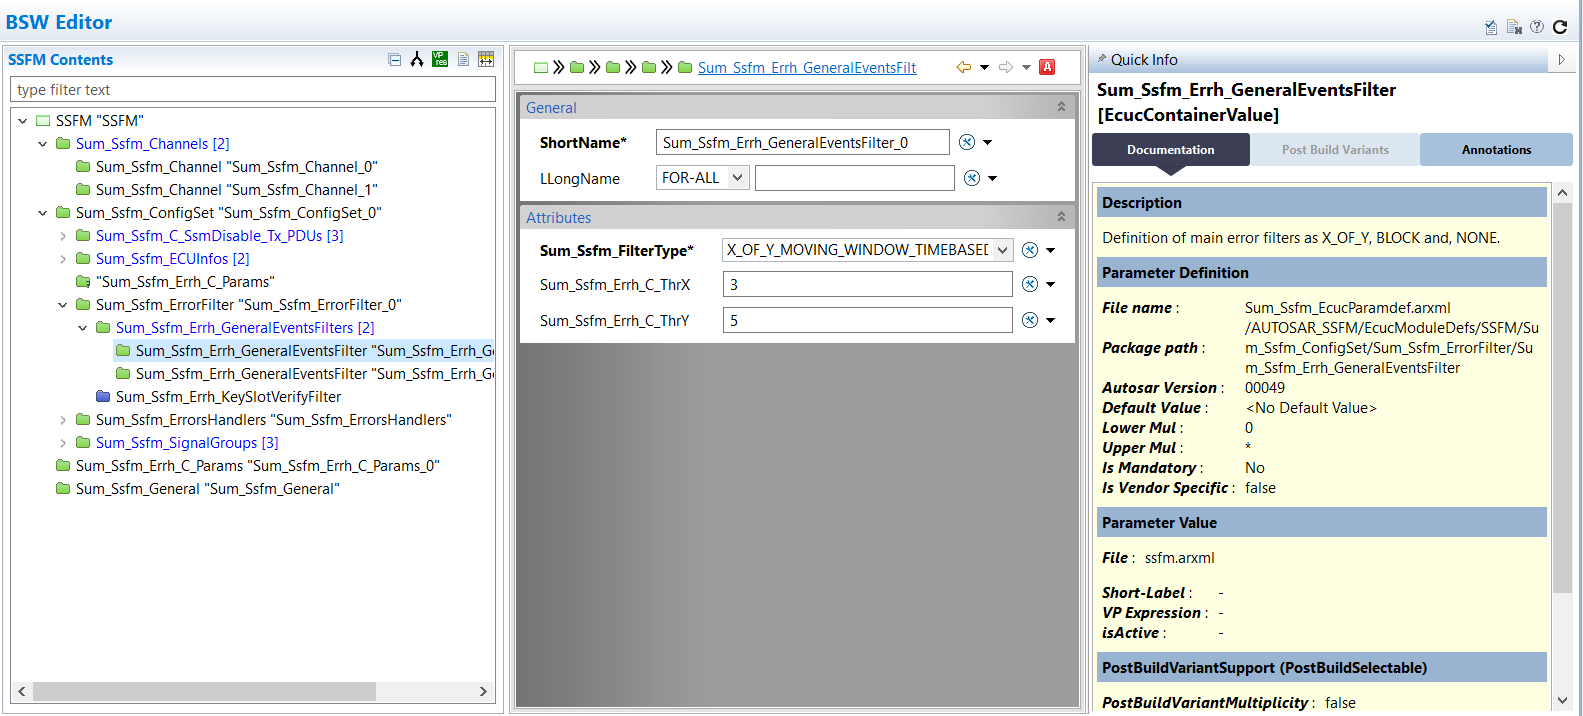
\includegraphics[scale=0.40]{images/GeneralEventFilter.PNG}
\end{figure}

\paragraph{BatteryVoltageRangeMinToMax interface}
The BatteryVoltageRangeMinToMax interface should be properly connected as described in \ref{subsec:DTCEnableCriteria}. In case of the OBD support, the
functionality of U19A6 57 will be enabled if the battery voltage is not less than the normal range. On the other hand, in case of no OBD support, the
battery voltage should be explicitly in the normal range to have the U19A6 57 functionality enabled.

\paragraph{SrvcMgr\_SSFM\_SrvcDscvryFlr\_U19A6\_57 interface}
The SrvcMgr\_SSFM\_SrvcDscvryFlr\_U19A6\_57 interface should be connected in order to support the DTC U19A6 57. The service discovery failure status will be received through this boolean interface from the SrvcMgr module.

\paragraph{SetEventStatus}
The SetEventStatus C/S operation (DiagnosticMonitor C/S interface) shall be connected to the \texttt{RP\_Dem\_SSFM\_DTC\_U19A6\_57} to let the SSFM notify the Dem module when needed.

\begin{figure}[H]
    \centering
    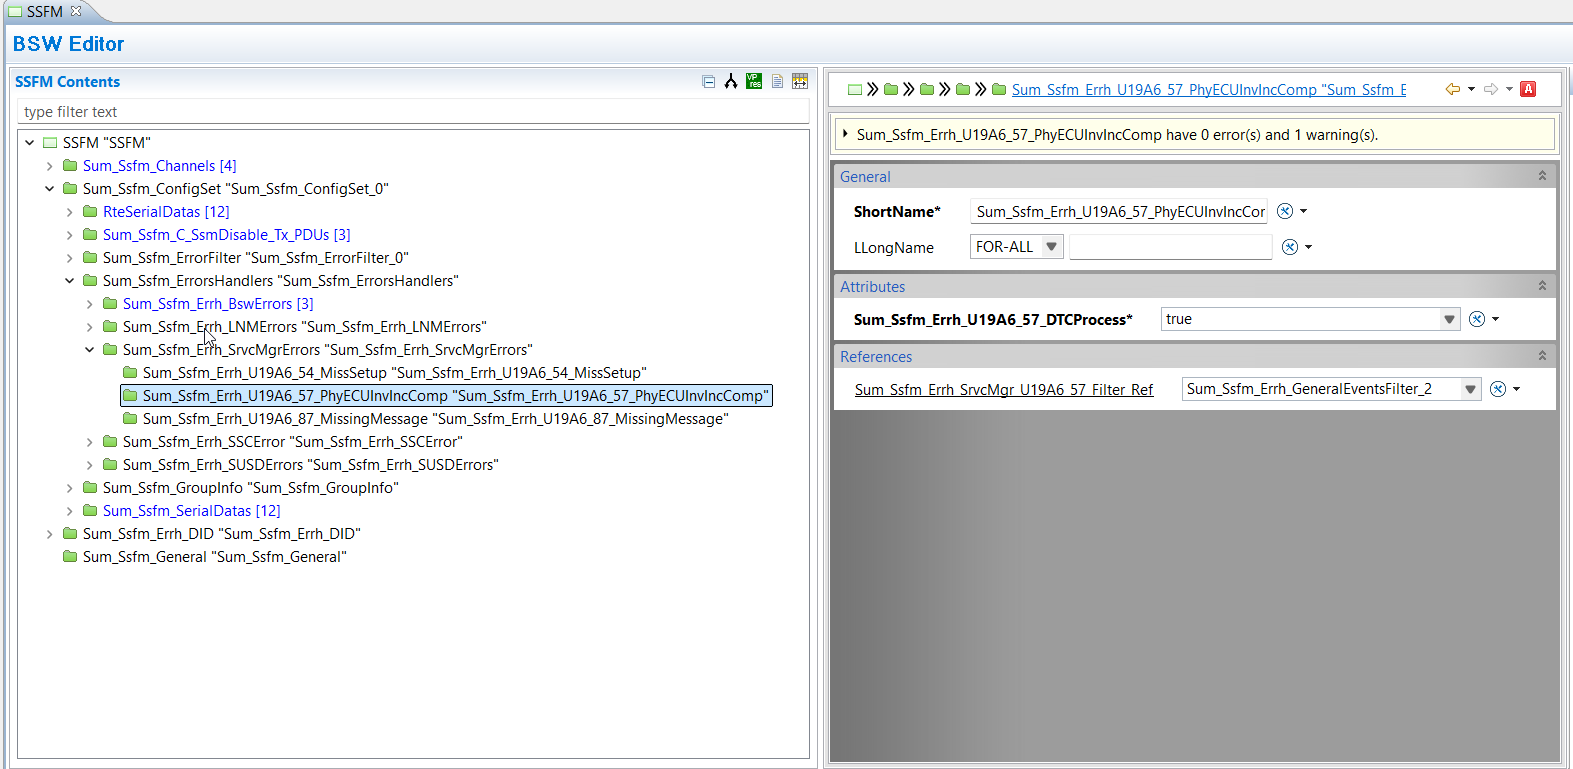
\includegraphics[scale=0.40]{images/U19A6_57_ServiceDiscoveryFailure.PNG}
    \caption{Configuration for U19A6\_57 Service Discovery Failure DTC}
\end{figure}

\subsection{DTC U19A3 8A}
\label{subsec:SSFMERRHDTCU19A38AHandler}
The DTC U19A3 8A indicates the Control Module Security Peripheral - Authentication Failure Diagnostic Status.

\paragraph{Sum\_Ssfm\_Errh\_CodeGen\_Enabled}
This is present in Sum\_Ssfm\_Errh\_U19A3\_CntrlModSecPer\_AuthFailure in the SSFM module to enable/disable the generation of the DTC U19A3 8A handler code. The parameter needs to be set to True.

\paragraph{Sum\_Ssfm\_Errh\_KeySlotVerifyFilter}
This contains all the general configuration parameters for Key Slot Verify Error Handlers. It needs to be configured.

\begin{figure}[H]
	\centering
	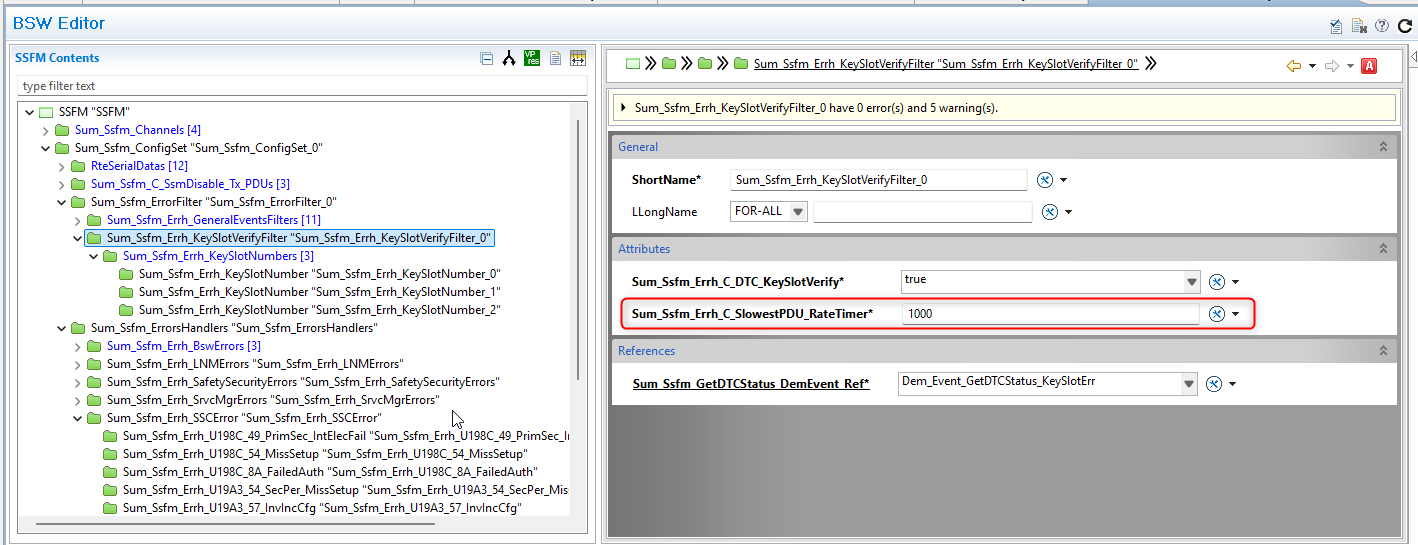
\includegraphics[scale=0.40]{images/KeySlotVerifyFilter.PNG}
\end{figure}

\paragraph{Sum\_Ssfm\_Errh\_KeySlotNumber}
This contains queue length for each keyslotverify. It need to be configured.

\paragraph{Sum\_Ssfm\_Errh\_C\_FailedAuthenticationTimer}
This parameter defines the maximum time that the number of MAC verification failures for a specific key slot remains greater than zero. Once the specified timer is exceeded, the test is considered to have failed.
Prior to exceeding the specified timer, upon receiving a passing frame on a specific key slot, the number of failures would be set to zero, and at this time, the timer would stop incrementing and be set to 0.

\paragraph{Sum\_Ssfm\_Errh\_C\_SlowestPDU\_RateTimer}
This parameter is used as the basis to determine when frames are not being received in this keyslot. This calibration shall be set equal to or greater than the periodic rate of the slowest PDU received in this keyslot.
It can stop decrementing the authentication window timer or increasing the failed authentication timer.

\begin{figure}[H]
	\centering
	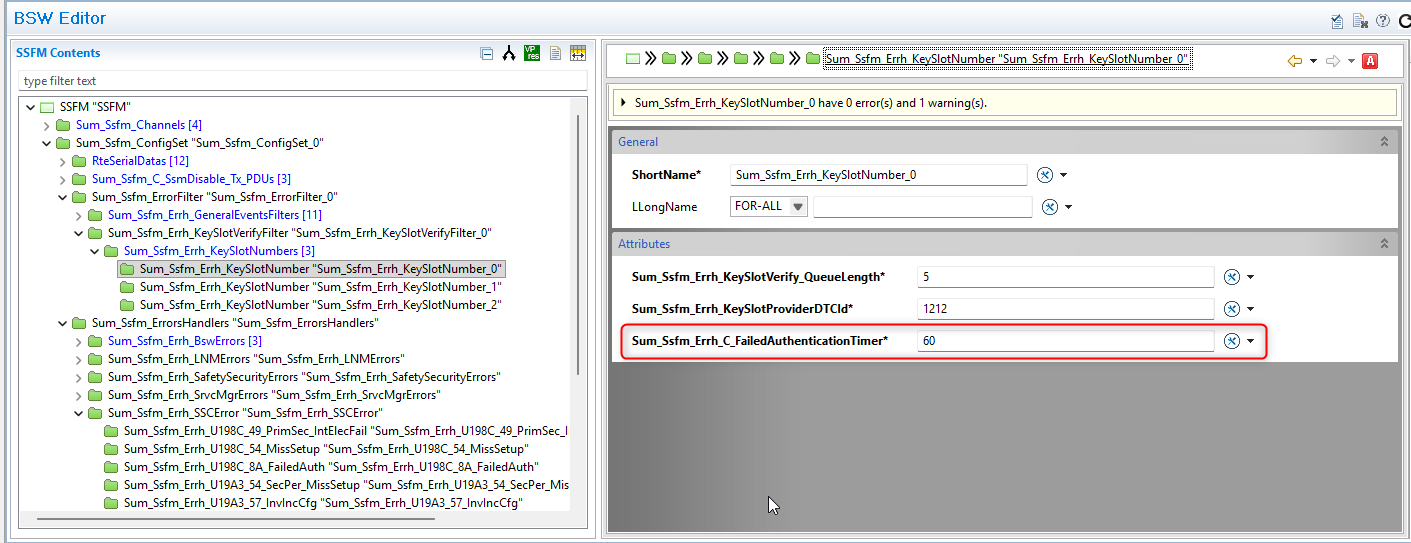
\includegraphics[scale=0.40]{images/KeySlotNumber.PNG}
\end{figure}

\paragraph{Sum\_Ssfm\_KeySlotVerify\_RunnablePeriodicity}
The periodicity parameter sets the period in which the runnable responsible for handling the key slot verification is called.
In order to have no drift and no missed verification, make sure that the parameter value is divisible by the above timers (Sum\_Ssfm\_Errh\_C\_FailedAuthenticationTime, Sum\_Ssfm\_Errh\_C\_SlowestPDU\_RateTimer).
The Sums will check for this compatibility at generation time using the default value set for the calibration parameter. 
However, it's up to the user to make sure that the periodicity remains divisible by the calibration values during the runtime.

\paragraph{BatteryVoltageRangeMinToMax interface}
The BatteryVoltageRangeMinToMax interface should be properly connected as described in \ref{subsec:DTCEnableCriteria}. In case of OBD support the
functionality of U19A3 8A will be enabled if the battery voltage is not less than the normal range. On the other hand, in case of no OBD support, the
battery voltage should be explicitly in the normal range to have the U19A3 8A functionality enabled.

\paragraph{SetEventStatus}
The SetEventStatus C/S operation (DiagnosticMonitor C/S interface) shall be connected to the \\\code{RP\_Dem\_SSFM\_DiagnosticMonitor\_SSC\_E\_KeySlotVerifyError} to let the SSFM notify the Dem module when needed.\\
The Port \code{RP\_SSC\_SSFM\_U19A3\_8A\_KeyProvisioned} needs to be connected to the SSC Port to receive notifications when the successful completion of key provisioning.

\subsection{DTC U198C 54}
\label{subsec:SSFMERRHDTCU198C54Handler}

The DTC U198C 54 indicates the Primary Security Information - Missing Setup/Learn.
It should be noted that the parameter Sum\_Ssfm\_Errh\_CodeGen\_Enabled can be configured as true or false; by setting it to false, the SSFM module will not propagate this DTC.

\paragraph{Sum\_Ssfm\_Errh\_C\_DTC\_U198C\_54\_MissSetup }
In order to enable the DTC U198C 54, the designated calibration parameter should be set to \code{true}.

\paragraph{Sum\_Ssfm\_Errh\_SSC\_U198C\_54\_EventFilter\_Ref} 
Setting the reference to the event filter for 198C\_54 error.
To get the reference to the general event filter, the user should configure the \\Sum\_Ssfm\_GeneralEventFilter used for 198C\_54.

\paragraph{BatteryVoltageRangeMinToMax interface}
The BatteryVoltageRangeMinToMax interface should be properly connected as described in \ref{subsec:DTCEnableCriteria} in order to respect its timing criteria.

\paragraph{SSC\_ERRH\_DTC\_198C\_54\_Status}
The SSC\_ERRH\_DTC\_198C\_54\_Status interface shall be connected to the SSC in order to receive notification about change of the status of the DTC U198C 54.

\paragraph{SetEventStatus}
The SetEventStatus C/S operation (DiagnosticMonitor C/S interface) shall be connected to the \\\code{RP\_Dem\_SSFM\_DTC\_U198C\_54} to let the SSFM notify the Dem module when needed.


\subsection{DTC U198C 49}
\label{subsec:198C49Handler}

The DTC U198C 49 indicates the failure regarding the Primary Security Information – Internal Electronic Failure (Key Provisioning).

It should be noted that the parameter Sum\_Ssfm\_Errh\_U198C\_49\_DTCProcess can be configured as true or false; by setting it to false, the SSFM module will not propagate this DTC.

\paragraph{Sum\_Ssfm\_Errh\_U198C\_49\_DTCProcess} 
In order to enable the DTC U198C 49, the designated calibration parameter should be set to \code{true}.

\paragraph{Sum\_Ssfm\_Errh\_SSC\_U198C\_49\_Filter\_Ref} 
Setting the reference to event filter for 198C\_49 error.
To get the reference to the general event filter, the user should configure the \\Sum\_Ssfm\_GeneralEventFilter used for 198C\_49 as the example image below.

\begin{figure}[H]
	\centering
	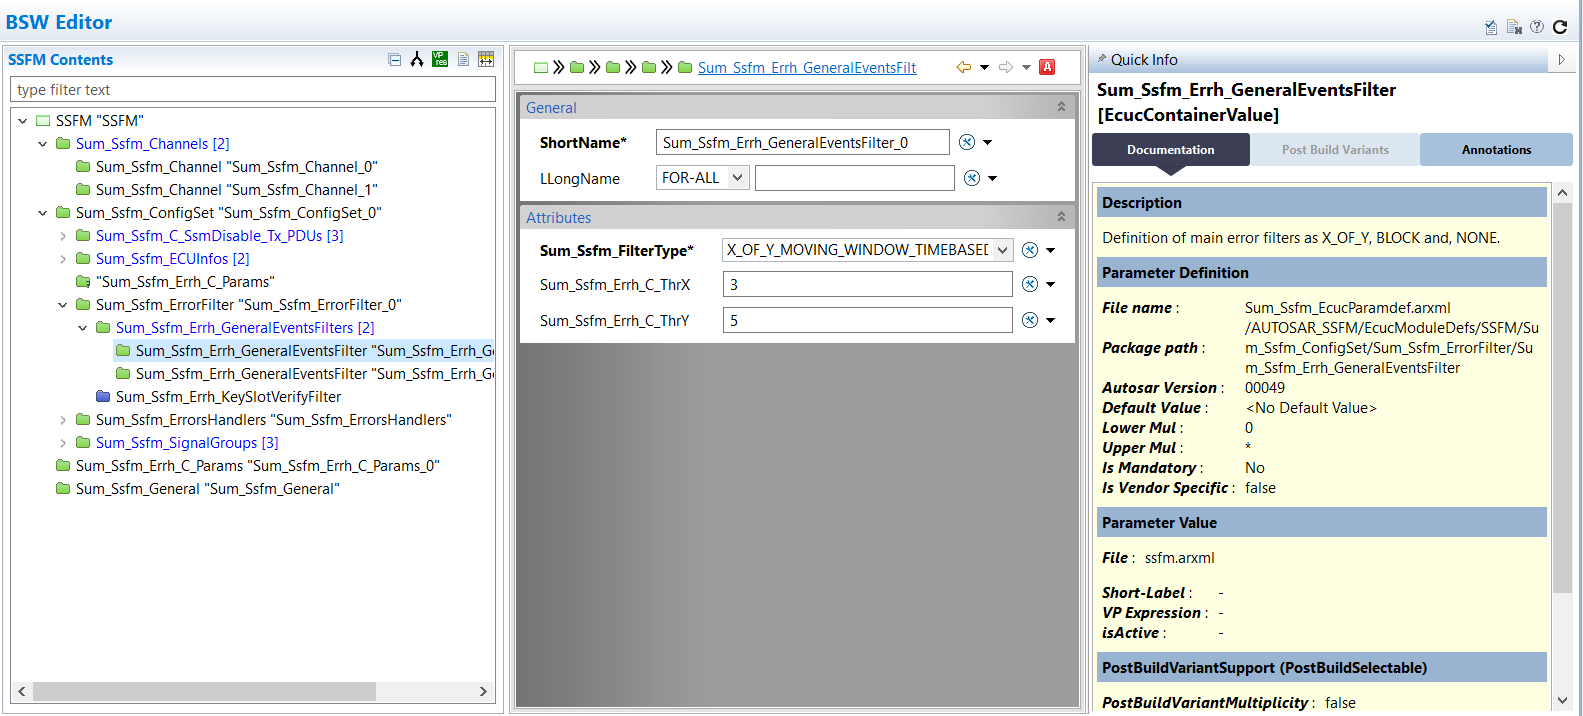
\includegraphics[scale=0.40]{images/GeneralEventFilter.PNG}
\end{figure}

\paragraph{BatteryVoltageRangeMinToMax interface}
The BatteryVoltageRangeMinToMax interface should be properly connected as described in \ref{subsec:DTCEnableCriteria}. Both timer flags must be TRUE for the DTC to be processed.

\paragraph{SetEventStatus}
The SetEventStatus C/S operation (DiagnosticMonitor C/S interface) shall be connected to the \texttt{RP\_Dem\_SSFM\_DTC\_U198C\_49} to let the SSFM notify the Dem module when needed.

\begin{figure}[H]
    \centering
    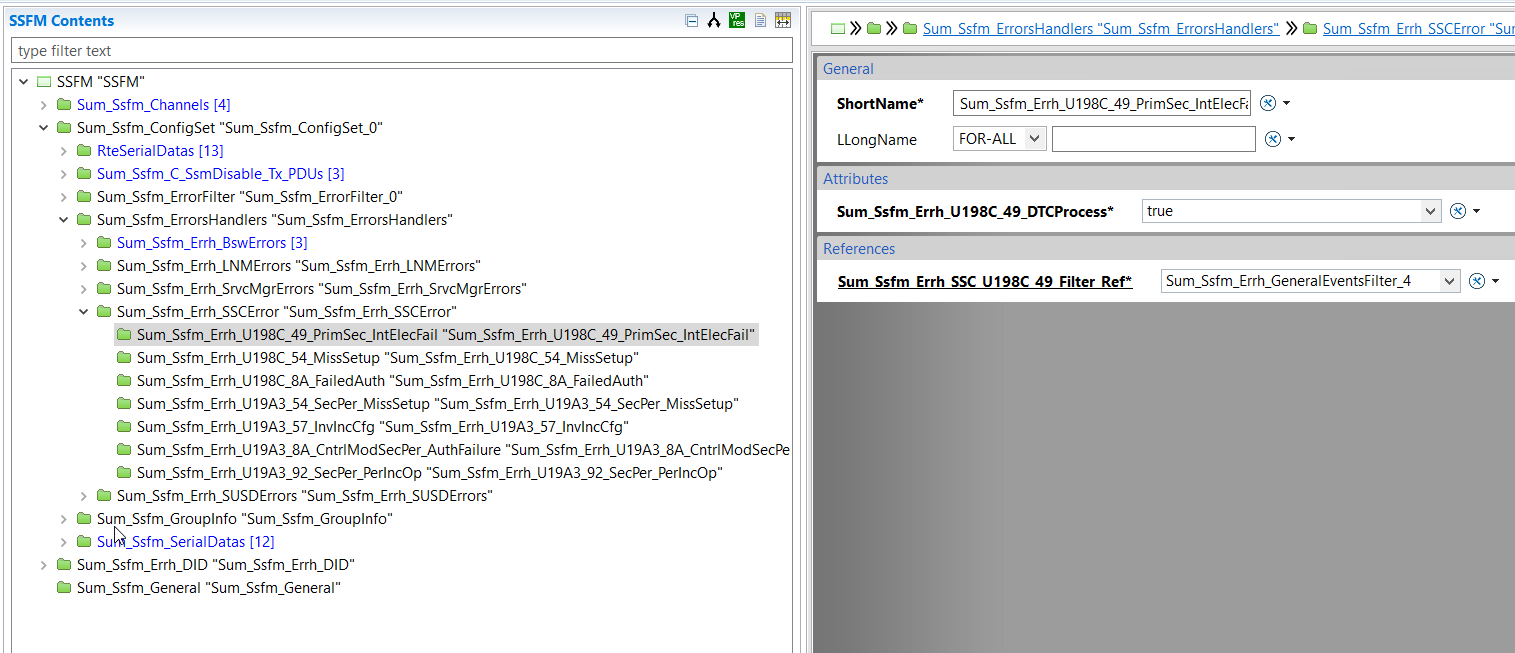
\includegraphics[scale=0.40]{images/U198C49_KeyProvisioning.PNG}
    \caption{Configuration for U198C\_49 Key Provisioning DTC}
\end{figure}


\subsection{DTC U198C 8A}
\label{subsec:SSFMERRHDTCU198C8AHandler}

The DTC U198C 8A indicates the Primary Security Information - Authentication Failure.
It should be noted that the parameter Sum\_Ssfm\_Errh\_CodeGen\_Enabled can be configured as true or false; by setting it to false, the SSFM module will not propagate this DTC.

\paragraph{Sum\_Ssfm\_VehicleRegion\_SerialData\_Ref}
This is the reference to the SerialData which contains the vehicle region information. This information is used to determine the enable criteria for DTC U198C 8A.

\paragraph{BatteryVoltageRangeMinToMax interface}
The BatteryVoltageRangeMinToMax interface should be properly connected as described in \ref{subsec:DTCEnableCriteria}. In case of the OBD support the
functionality of U198C 8A will be enabled if the battery voltage is not less than the normal range. On the other hand, in case of no OBD support, the
battery voltage should be explicitly in normal range to have the U198C 8A functionality enabled.

\paragraph{Sum\_Ssfm\_Errh\_SSC\_U198C\_8A\_EventFilter\_Ref}
Setting the reference to the event filter for U198C\_8A error.
To get the reference to the general event filter, the user should configure the \\Sum\_Ssfm\_GeneralEventFilter used for 198C\_8A.

\paragraph{SSC\_ERRH\_DTC\_198C\_8A\_Status}
The SSC\_ERRH\_DTC\_198C\_8A\_Status interface shall be connected to the SSC in order to receive notification about change of the status of the DTC U198C 8A.

\paragraph{SetEventStatus}
The SetEventStatus C/S operation (DiagnosticMonitor C/S interface) shall be connected to the RP\_Dem\_SSFM\_DTC\_U198C\_8A to let the SSFM notify the Dem module when needed.

\paragraph{Setting calibration parameter process DTC Sum\_Ssfm\_Errh\_C\_DTC\_KeySlotVerify}
In order to enable the DTC U19A3 8A, the designated calibration parameter should be set to \code{true}.

\paragraph{Setting calibration parameter Sum\_Ssfm\_Errh\_C\_FailedAuthenticationTimer}
In order to define the maximum time in second that the number of MAC verification failures for all key slot greater than zero.

\paragraph{Setting calibration parameter Sum\_Ssfm\_Errh\_C\_PassedAuthenticationTimer}
In order to define the maximum time in second that the number of MAC verification failures for all key slot equal to zero.

\paragraph{Setting calibration parameter Sum\_Ssfm\_Errh\_C\_SlowestPDU\_RateTimer}
In order to define the maximum time when frames are not being received in a keyslot in millisecond to stop increasing pass/failed authentication timer.

\paragraph{Setting the runnable periodicity parameter Sum\_Ssfm\_KeySlotVerify\_RunnablePeriodicity}
The periodicity parameter sets the period in which the runnable responsible for handling the key slot verification is being called.
In order to have no drift and no missed verification, make sure that the parameter value is divisible by the above timers (FailedAuthenticationTimer, PassedAuthenticationTimer, and SlowestPDU\_RateTimer).
The Sums will check for this compatibility at generation time using the default value set for the calibration parameter. However, it's upon user to make sure that the periodicity remains divisible by the calibration values during the runtime.

\paragraph{Setting the reference to the Dem event in the Sum\_Ssfm\_GetDTCStatus\_DemEvent\_Ref \\parameter}
To obtain the Dem event reference for KeySlot Verify Error, the user must configure the DemEventParameter, related to the event, present within the DEM. It is also important to configure the DemDTC associated with the event, as this will be referenced in the DemDTCRef present in the DemEventParameters.

\begin{figure}[H]
	\centering
	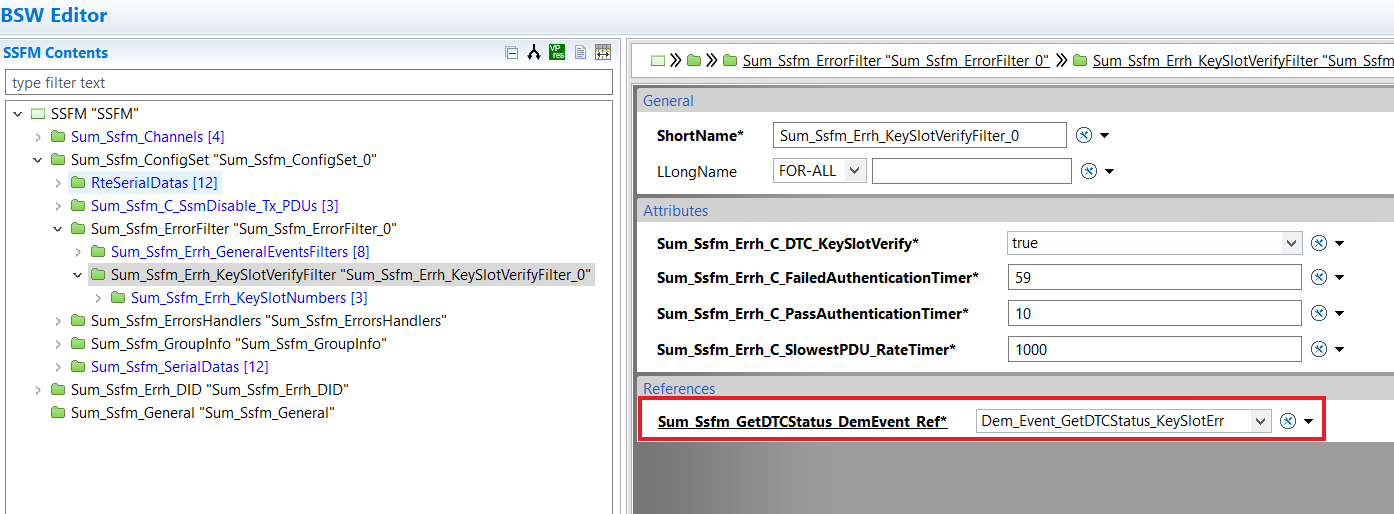
\includegraphics[scale=0.40]{images/KeySlotVerifyError.PNG}
\end{figure}

\paragraph{Setting Sum\_Ssfm\_Errh\_KeySlotVerify\_QueueLength}
In order to define the queue length for each KeySlot to support multiple messages authentication.
Hint: set the parameter at least the number of authenticated messages for each KeySlot.

\paragraph{BatteryVoltageRangeMinToMax interface}
The BatteryVoltageRangeMinToMax interface should be properly connected as described in \ref{subsec:DTCEnableCriteria}. In case of the OBD support the
functionality of U19A3 8A will be enabled if the battery voltage is not less than the normal range. On the other hand, in case of no OBD support, the
battery voltage should be explicitly in normal range to have the U19A3 8A functionality enabled.

\paragraph{BswM configuration}
The SSFM component includes the RPort RP\_BswM\_SSFM\_SecPError for receiving the HSM error notification from BswM. In order to process keyslotverify error, SecPError status is needed to be no error.

\paragraph{Setting Dem Callback DTC Status Changed}
The user shall also configure a \textbf{DemCallbackDTCStatusChanged} instance under the Dem General Configuration with a callback function named as \textbf{Ssfm\_Dem\_CB\_DTCStatusChanged} to enable the DTC setting feature.

\subsection{Value of Signal Protection Calculation Incorrect DTC UXXXX83}
\label{subsec:UXXXX83}

\paragraph{Checking calibration parameter process DTC} 
To control the DTC for incorrect values of signal protection calculation by reading configured calibration parameters.(Sum\_Ssfm\_Errh\_C\_DTC\_UXXXX\_83\_SignalProtectionIncorrect).


\begin{figure}[H]
	\centering
	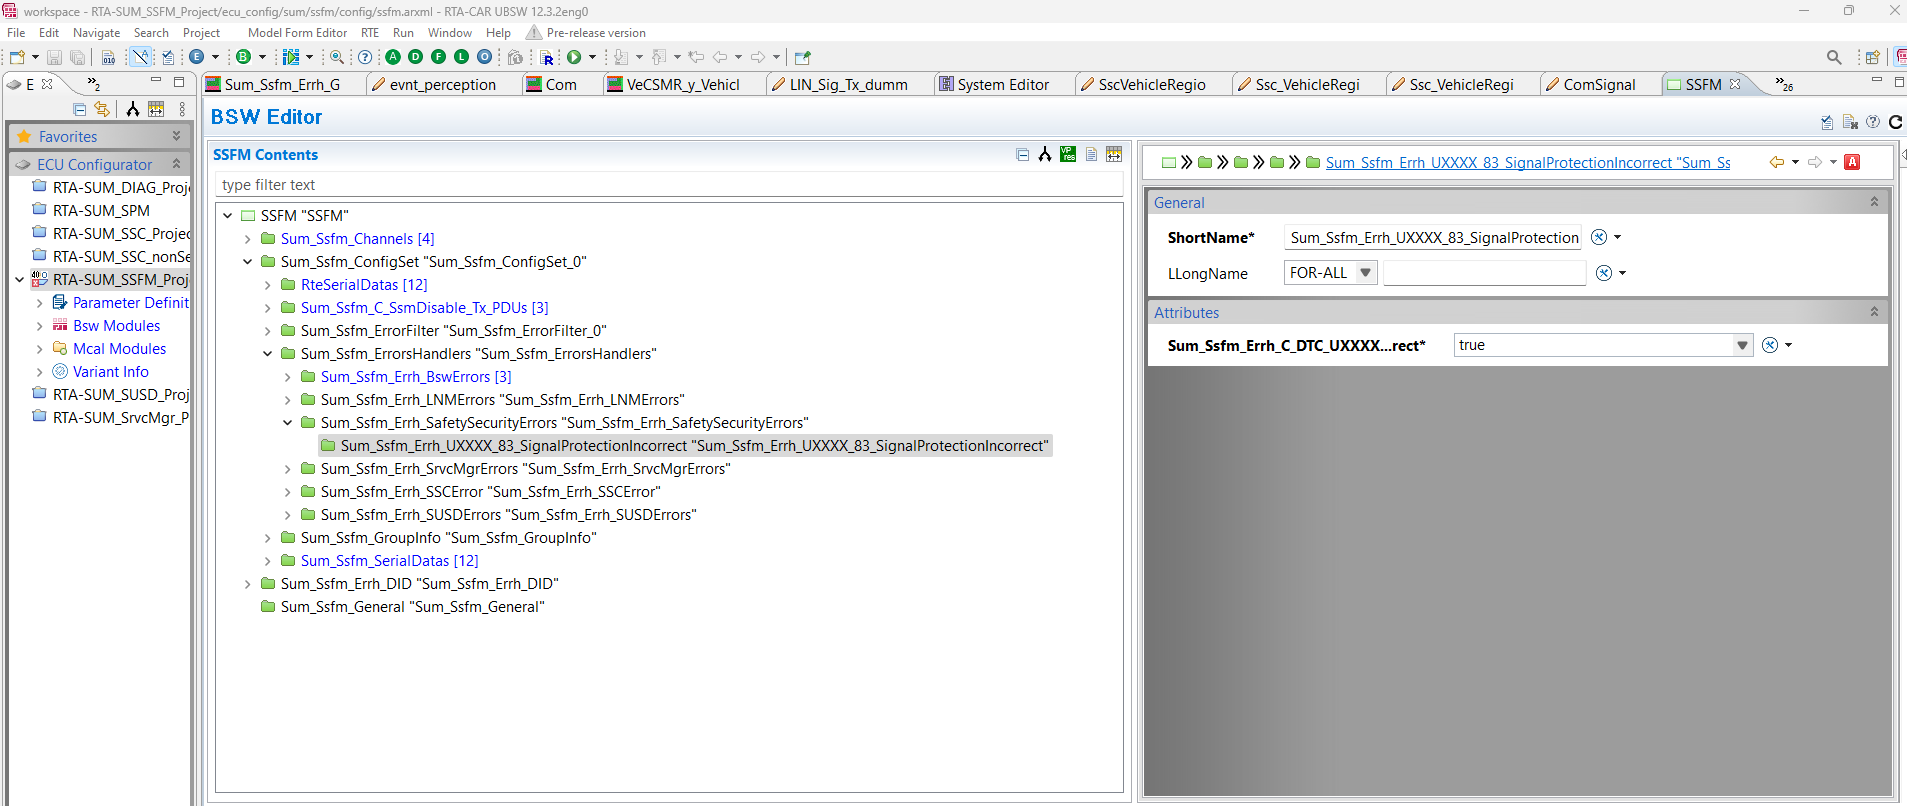
\includegraphics[scale=0.40]{images/UXXXX83Error.PNG}
\end{figure}

\subsection{Run Crank Input Fault Indication Manager}
\label{subsec:RunCrankInputFaultIndicationManager}

The Run Crank Input Fault Indication Manager is responsible for the following tasks:

\begin{enumerate}
    \item Receive the notifications from SUM\_SUSD to request setting or clearing the corresponding DTC from Dem.
    \item Notify Dem of the debouncing result.
    \item Receive the DTC status then confirm the setting of DTC associate with run crank input stuck diagnostic from Dem.
    \item Notify SUM\_SUSD of the run crank input stuck diagnostic DTC.
\end{enumerate}

\paragraph{Checking calibration parameter process DTC} 
To control the process DTC for run crank input stuck high and low indication via reading configured calibration parameter (Sum\_Ssfm\_Errh\_C\_DTCProcess\_<n>).

\paragraph{Setting the reference to event filter for run crank input stuck high indication}
To get the reference to the general event filter, the user should configure the \\Sum\_Ssfm\_GeneralEventFilter used for run crank input stuck high indication as the example image below.

\paragraph{Setting the reference to event filter for run crank input stuck low indication}
To get the reference to the general event filter, the user should configure the \\Sum\_Ssfm\_GeneralEventFilter used for run crank input stuck low indication as the example image below.

Note: Each of the error shall have the invidual instance of Sum\_Ssfm\_GeneralEventFilter. So the user needs to create each instance Sum\_Ssfm\_GeneralEventFilter for each error.

\begin{figure}[H]
	\centering
	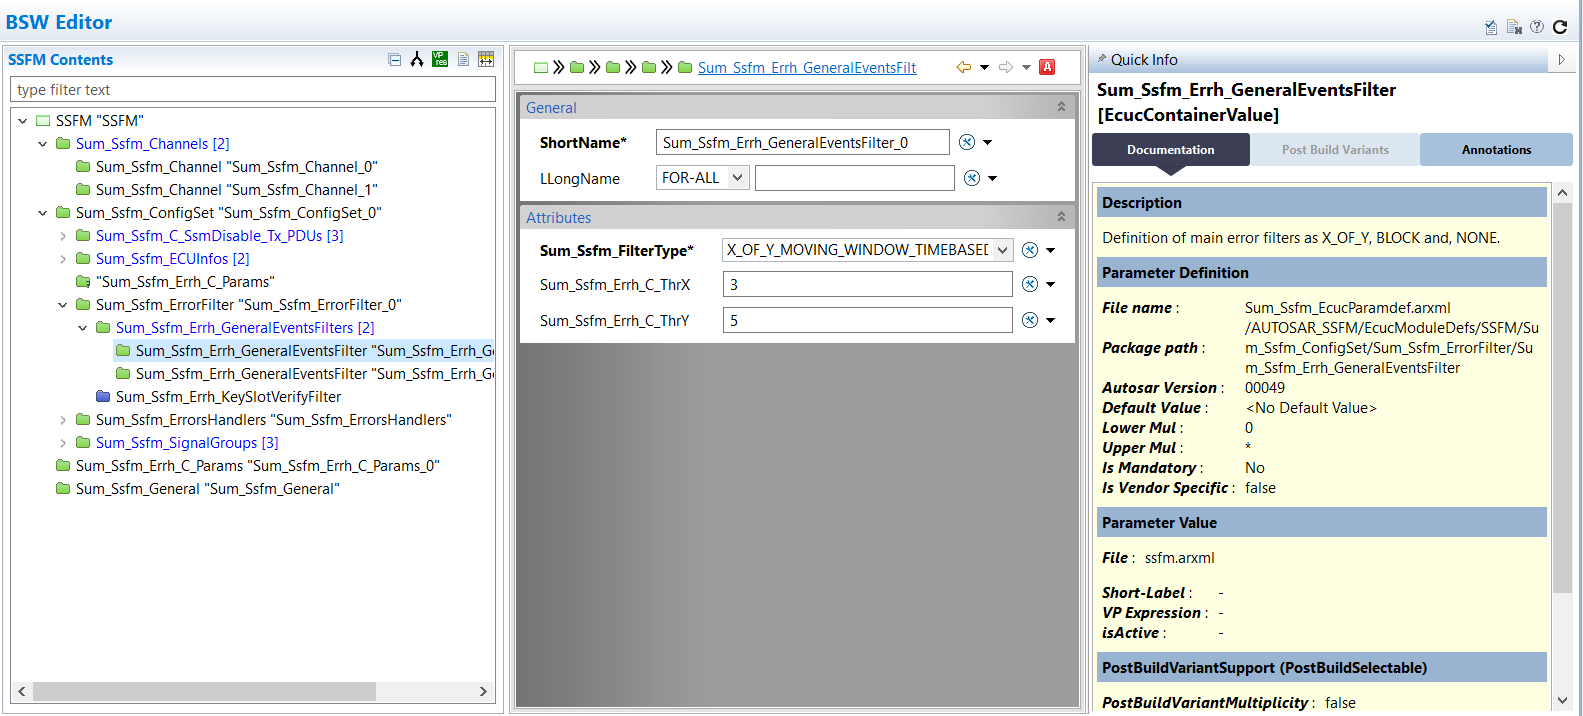
\includegraphics[scale=0.40]{images/GeneralEventFilter.PNG}
\end{figure}

\paragraph{Setting references to DEM events for run crank input stuck low and high indication}
To obtain references to the DEM events for both the run crank input stuck low and high indications, the user must configure the DemEventParameters related to each event present within the DEM. It is also important to configure the DemDTCs associated with the respective DTCs, as these will be referenced in the DemDTCRef present in the DemEventParameters for both low and high stuck input indications.

\begin{figure}[H]
	\centering
	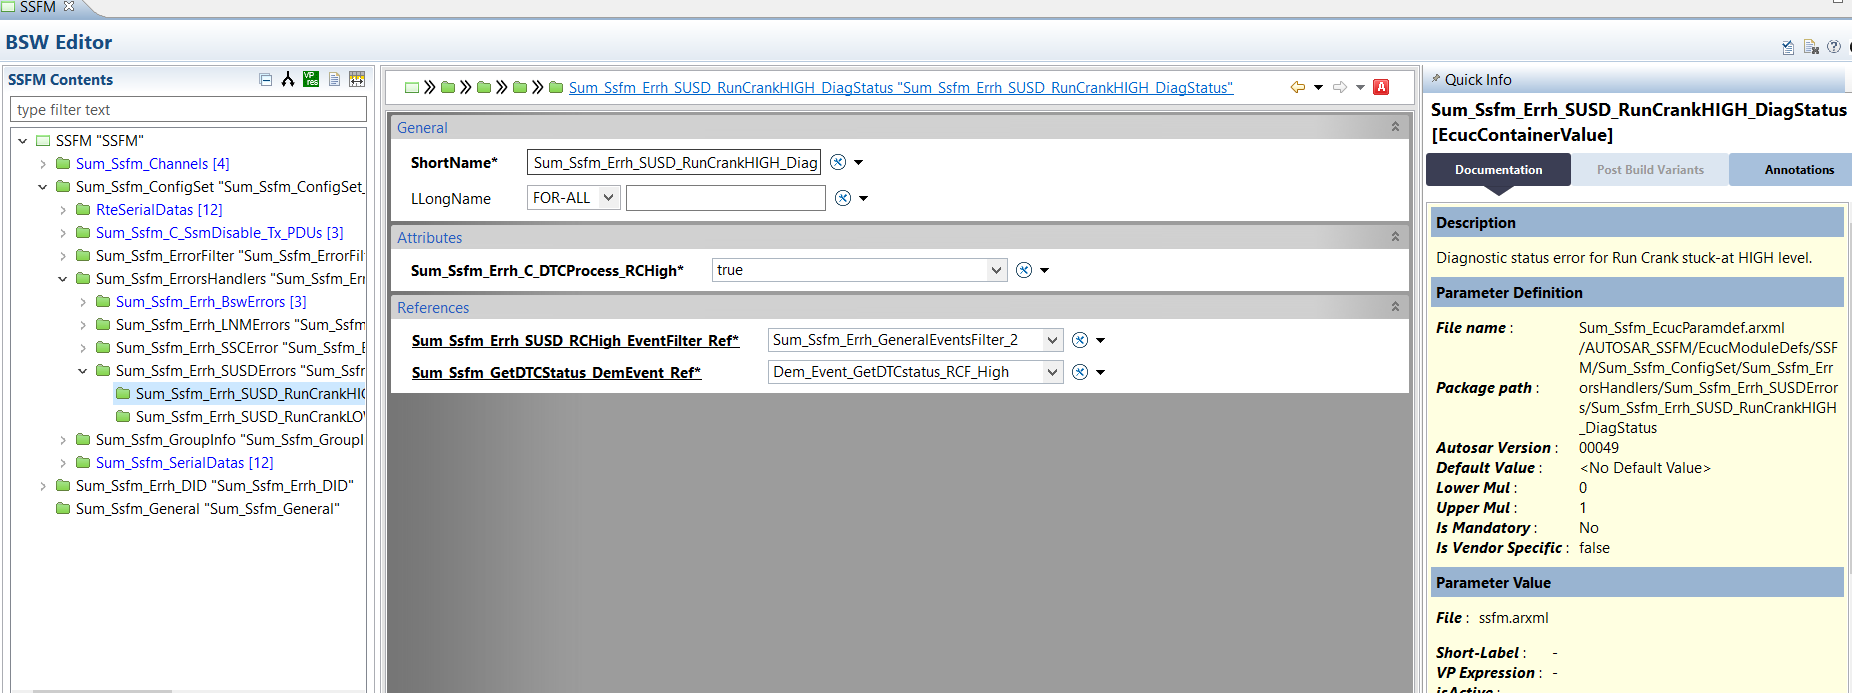
\includegraphics[scale=0.40]{images/RunCrankInputHighDiagSts.PNG}
\end{figure}

\begin{figure}[H]
	\centering
	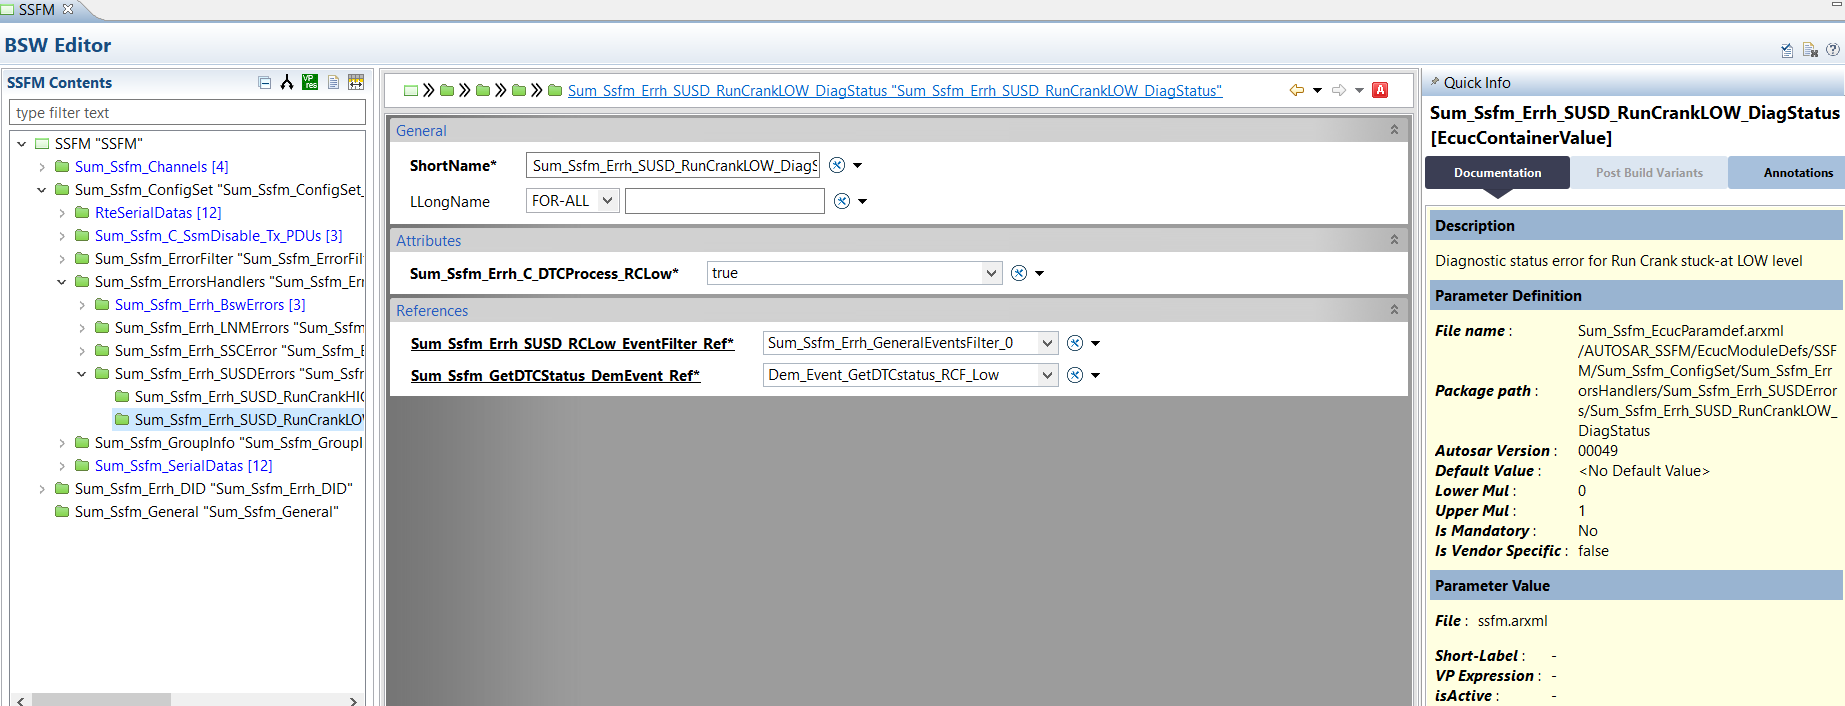
\includegraphics[scale=0.40]{images/RunCrankInputLowDiagSts.PNG}
\end{figure}

\paragraph{Setting Dem Callback DTC Status Changed}
The user shall also configure a \textbf{DemCallbackDTCStatusChanged} instance under the Dem General Configuration 
with a callback function named as \textbf{Ssfm\_Dem\_CB\_DTCStatusChanged} to enable the DTC setting feature.


\subsection{DID Handlers}
\subsubsection{DID 0xE0B9}
\label{subsec:DID 0xE0B9}

This function is enabled by default and requires the Sum\_Ssfm\_Os\_Counter\_1ms\_Ref parameter to be configured with an SSFM dedicated 1ms Os Counter.
To configure this DID in Dcm, assure that in the configured \code{DcmDspDid} the \code{DcmDspDidIdentifier} parameter is set to 57529 Decimal, or 0xE0B9 Hex. 
\begin{figure}[H]
	\centering
	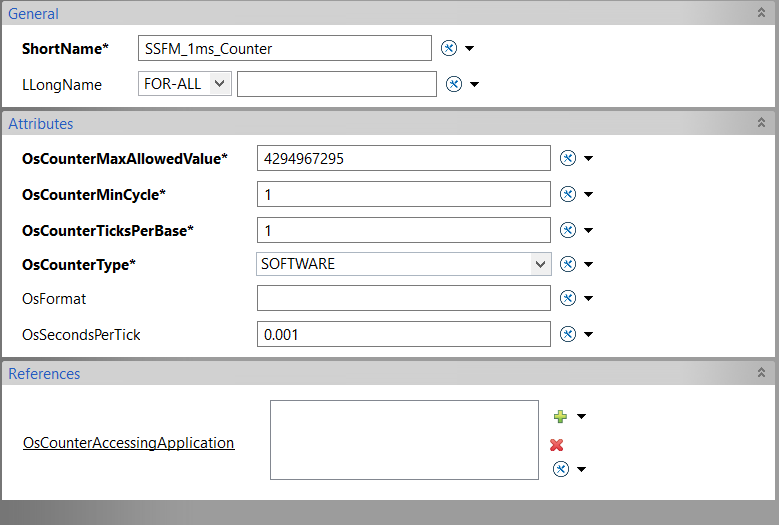
\includegraphics[scale=0.40]{images/os_counter.PNG}
\end{figure}


All the CAN/ETH SerialDatas defined in SSFM must have the \code{Sum\_Ssfm\_MessageID\_Ref} configured to access to the message id.
Please note that the messages in the list can be in any order. To find out the oldest unavailable message refer to the time since it is unavailable.

The DID data must be saved in non-volatile memory: connect the port PS\_NvM\_SUM\_SSFM\_Sum \_Ssfm\_E0B9\_Array from the NvM module to the RP\_NvM\_SSFM\_NvMService\_DID\_E0B9\_Data SSFM's port. Please, 
take into account the fact that the PS\_NvM\_SUM\_SSFM\_Sum\_Ssfm\_E0B9\_Array port will be generated after BSW generation subsequently to Confgen step. 

The Sum\_Ssfm\_SigStsInfoLossOfCommNvmRef parameter in the Sum\_Ssfm\_NvM\_References sub-container shall be configured to refer to the NVM blocks where the DID E0B9 data stored. 
\begin{figure}[H]
	\centering
	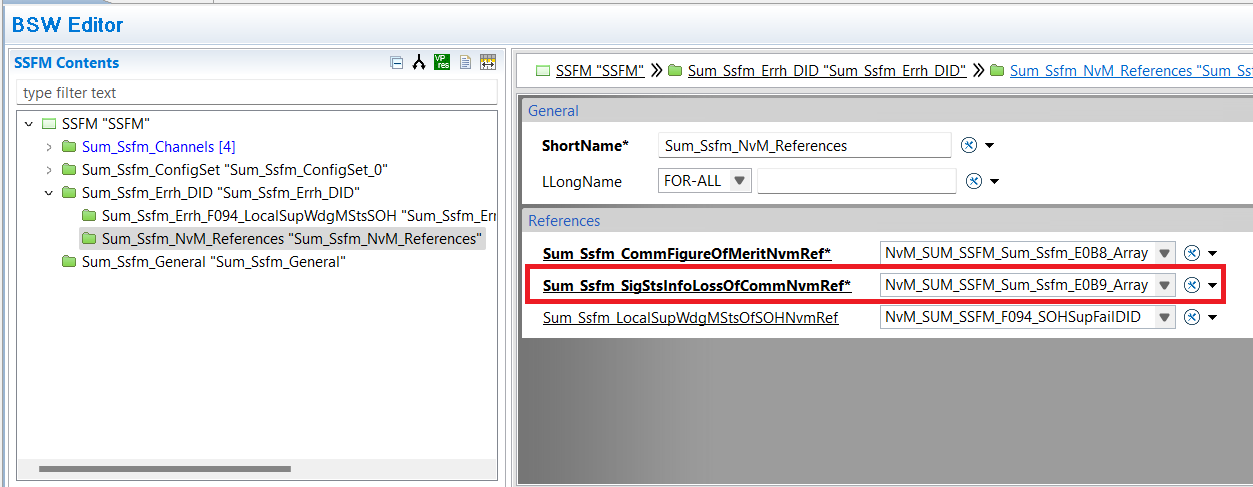
\includegraphics[scale=0.40]{images/NvMBlock_DID_E0B9_Ref.PNG}
\end{figure}

The NvM block for DID 0xE0B9 will be generated during the Confgen step with the necessary information for SumCode generation.
\begin{figure}[H]
	\centering
	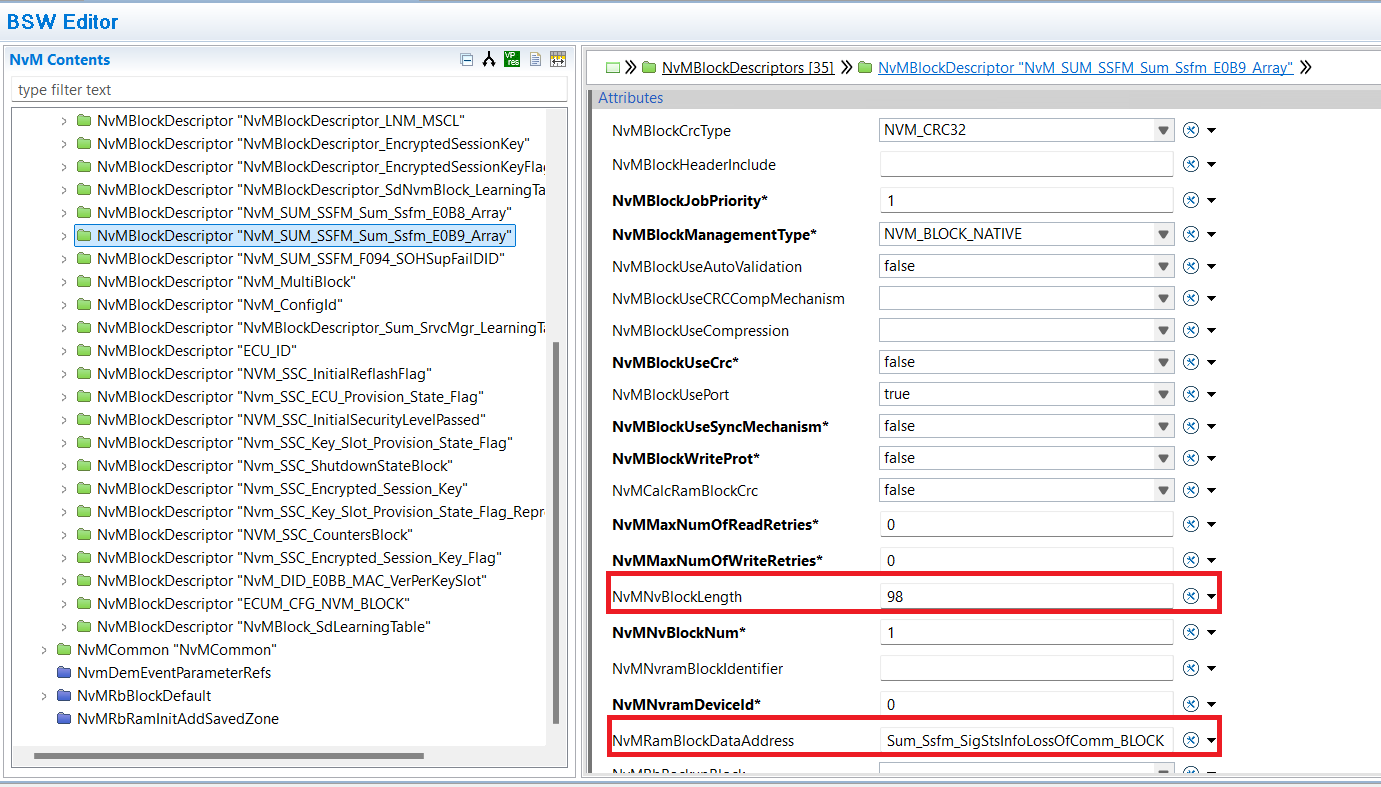
\includegraphics[scale=0.30]{images/NvMBlock_DID_E0B9.PNG}
\end{figure}

\subsubsection{DID 0xE0B8}
\label{subsec:DID 0xE0B8}

This function is enabled by default.
To configure this DID in Dcm, assure that in the configured \code{DcmDspDid} the \code{DcmDspDidIdentifier} parameter is set to 57528 Decimal, or 0xE0B8 Hex. 
Since the DID data must be saved in non-volatile memory, connect the port PS\_NvM\_SUM\_SSFM\_Sum \_Ssfm\_E0B8\_\newline\_Array from 
the NvM module to the RP\_NvM\_SSFM\_NvMService\_DID\_E0B8\_Data SSFM's port.
Take into account the fact that the PS\_NvM\_SUM\_SSFM\_Sum\_Ssfm\_E0B8\_Array 
port will be generated after BSW generation subsequently to Confgen step. 

The Sum\_Ssfm\_CommFigureOfMeritNvmRef parameter in the Sum\_Ssfm\_NvM\_References sub-container shall be configured to refer to the NVM blocks where the DID E0B8 data stored. 
\begin{figure}[H]
	\centering
	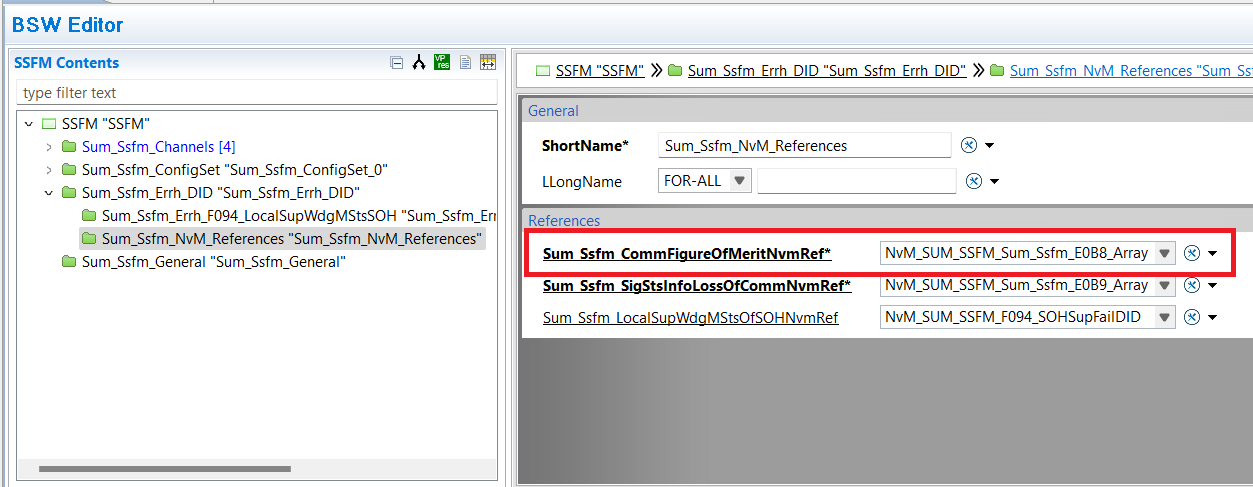
\includegraphics[scale=0.40]{images/NvMBlock_DID_E0B8_Ref.PNG}
\end{figure}

The NvM block for DID 0xE0B8 will be generated during the Confgen step with the necessary information for SumCode generation.
\begin{figure}[H]
	\centering
	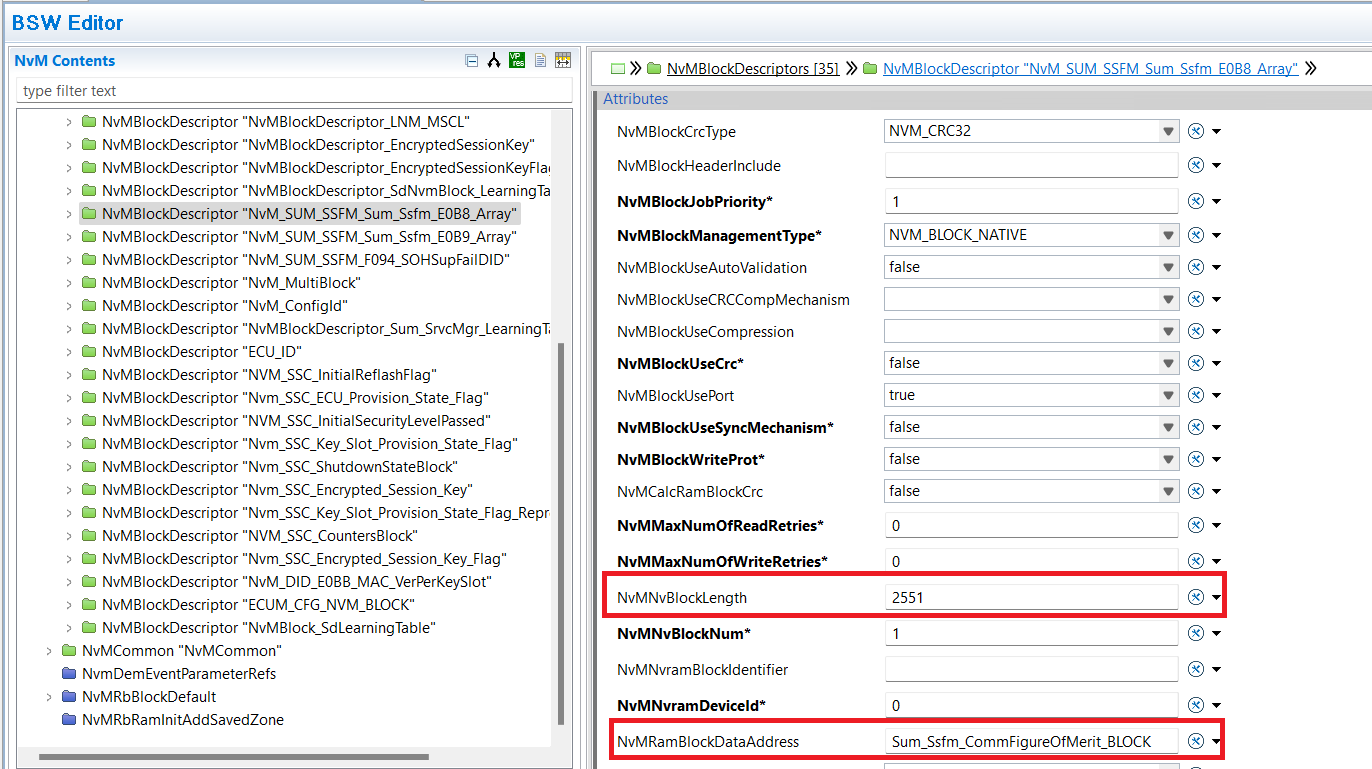
\includegraphics[scale=0.30]{images/NvMBlock_DID_E0B8.PNG}
\end{figure}

\paragraph{Configuration constraints for DID 0xE0B8}
The following constraints are enforced at code-generation time and will cause an error if violated:

\begin{enumerate}
	\item \textbf{DCM length format} -- The \code{DcmDspDataByteSize} configured for DID 0xE0B8 must satisfy the formula $\text{length} = 1 + N \times 10$, i.e.\ $(\text{length} - 1)$ must be divisible by~10.
	The value~1 accounts for a leading status byte; each of the $N$ entries occupies 10~bytes.
	A violation is reported as: \textit{``DCM DcmDspDataByteSize for DID 0xE0B8 is invalid: (length-1) must be divisible by 10 (required format: 1 + N*10).''}

	\item \textbf{DCM length range} -- The derived entry count $N = (\text{length} - 1) / 10$ must be within the range $[1,\,255]$.
	A violation is reported as: \textit{``DCM DcmDspDataByteSize for DID 0xE0B8 derives an entry count N out of valid range [1, 255] (required format: 1 + N*10).''}

	\item \textbf{NvM / DCM length consistency} -- The \code{NvMNvBlockLength} of the NvM block referenced for DID 0xE0B8 must equal the \code{DcmDspDataByteSize} (both must be $1 + N \times 10$).
	A violation is reported as: \textit{``NvM NvMNvBlockLength for DID 0xE0B8 does not match DCM DcmDspDataByteSize (both must equal 1 + N*10).''}
\end{enumerate}

\noindent These three checks are only active when DID 0xE0B8 is present in the configuration.

\subsubsection{DID 0xE0BA}
\label{subsec:DID0xE0BA}

This function handles Signal Protection Calculation Failure Counter and is enabled by default.
To configure this DID in Dcm, assure that in the configured \code{DcmDspDid} the \code{DcmDspDidIdentifier} parameter is set to 57530 decimal, or 0xE0BA hex.

SSFM provides a list of the last 16 SerialDatas with signal protection calculation failures (FPI and/or FOI failures). The DID E0BA maintains a priority-sorted list of up to 16 entries, where each entry contains:
\begin{itemize}
\item Message ID (4 bytes) - Identifier of the message experiencing protection failure
\item FOI Count (1 byte) - Continuous operation failure count
\item FPI Count (1 byte) - Signal protection failure count
\end{itemize}

The entries are automatically sorted by total failure count (FOI + FPI) in ascending order, with the lowest count entries appearing first. When the storage is full (16 entries), new entries with higher failure counts will replace existing entries with lower counts.

Since the DID data must be saved in non-volatile memory, connect the port PS\_NvM\_SUM\_SSFM\_Sum\_Ssfm\_E0BA\_Array from 
the NvM module to the RP\_NvM\_SSFM\_NvMService\_DID\_E0BA\_Data SSFM's port.
Take into account the fact that the PS\_NvM\_SUM\_SSFM\_Sum\_Ssfm\_E0BA\_Array 
port will be generated after BSW generation subsequently to Confgen step.

The Sum\_Ssfm\_SigProtectionCalcIncorrectNvmRef parameter in the Sum\_Ssfm\_NvM\_References sub-container shall be configured to refer to the NVM blocks where the DID E0BA data is stored.
\begin{figure}[H]
	\centering
	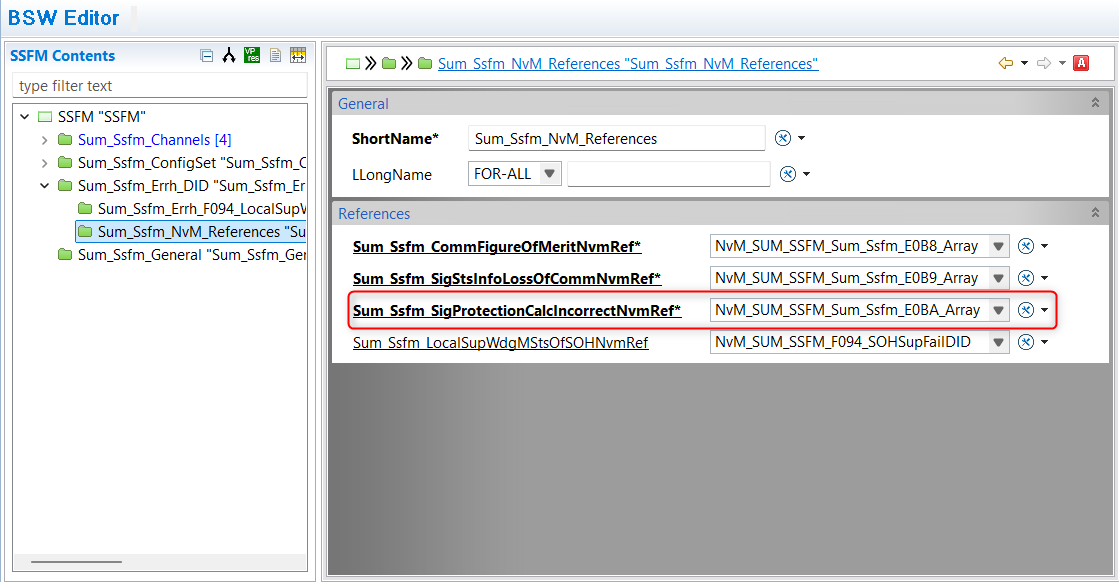
\includegraphics[scale=0.40]{images/NvMBlock_DID_E0BA_Ref.png}
\end{figure}

The NvM block for DID 0xE0BA will be generated during the Confgen step with the necessary information for SumCode generation.
\begin{figure}[H]
	\centering
	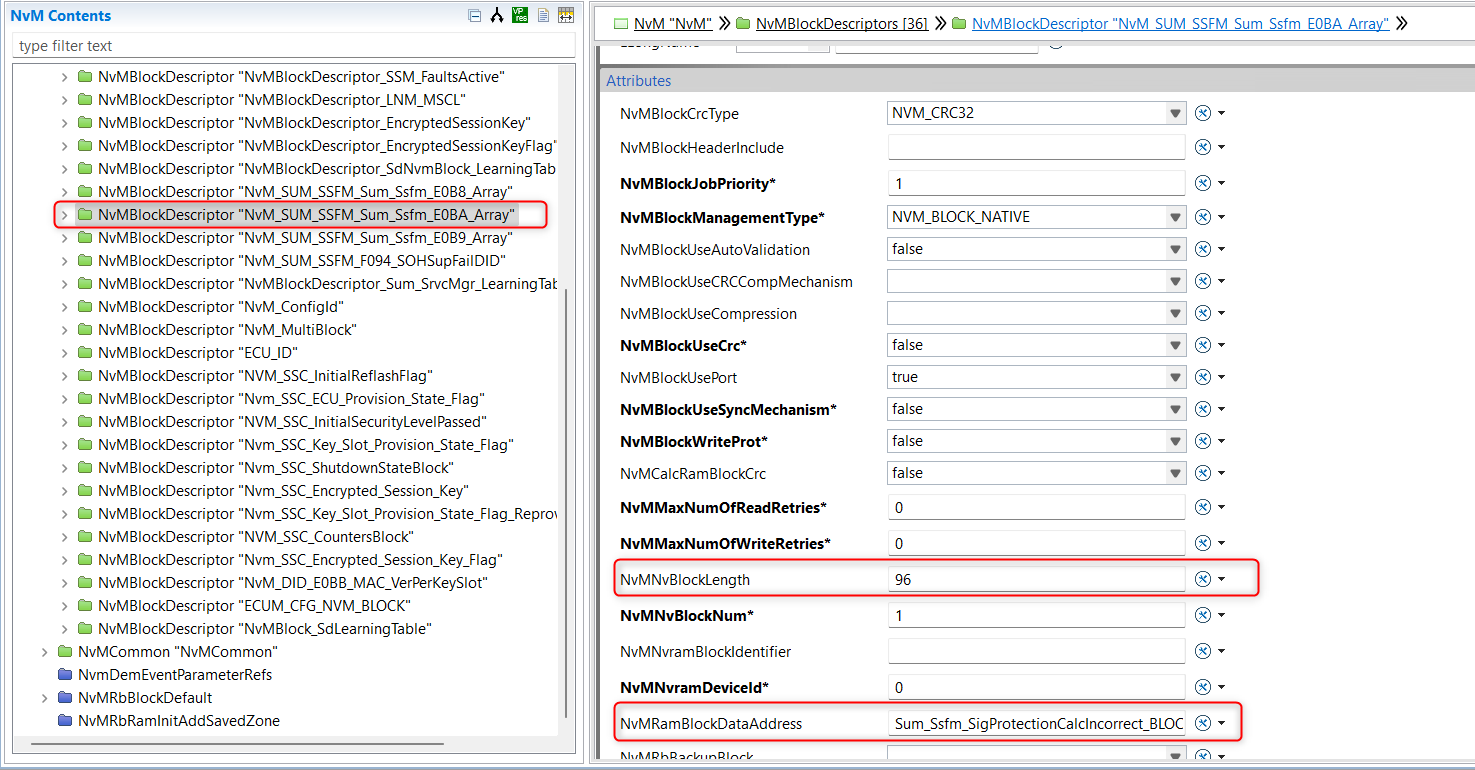
\includegraphics[scale=0.30]{images/NvMBlock_DID_E0BA.png}
\end{figure}

\subsubsection{DID 0xE0BB}
\label{subsec:DID 0xE0BB}
This function is enabled by default.
To configure this DID in Dcm, assure that in the configured \code{DcmDspDid} the \code{DcmDspDidIdentifier} parameter is set to 57531 Decimal, or 0xE0BB Hex. 

\textbf{Sum\_Ssfm\_Errh\_KeySlotProviderDTCId}

This parameter (one for each KeySlot) shall be configured with the DTC identifier of the ECU's provider message that uses this KeySlot.

Note: Key Slot 1 (ECU Unlock Key) shall not be included under the \code{Sum\_Ssfm\_Errh\_KeySlotNumber} container in the SSFM configuration.

\textbf{Runnable\_SSFM\_DID\_E0BB}

The Runnable\_SSFM\_DID\_E0BB is responsible for populating the diagnostic data identifier E0BB with KeySlot verification status information. When requested by the diagnostic service, this function performs the following operations:

\begin{itemize}
	\item Determines the number of supported KeySlots by rounding the configured KeySlot count up to the nearest supported value (0, 10, 20, 50, 100, 150, 200, or 255).
	\item Collects the verification status, DTC identifier, and failure timer for each configured KeySlot from the internal Sum\_Ssfm\_Errh\_KeySlotVerifyFilter[] buffer. The status values are: 0, 1, or 2.
	\item Appends unused entries with status 3 if the configured KeySlot count is less than the supported value, ensuring the response structure matches the expected format.
\end{itemize}

The Runnable\_SSFM\_DID\_E0BB\_ReadDataLength is responsible to provide the length of the payload that will be retrieved. 
The number of key slots supported determines the length of the DID:
\begin{itemize}
	\item 0 slots = 1 byte
	\item 10 slots = 28 bytes
	\item 20 slots = 58 bytes
	\item 50 slots = 148 bytes
	\item 100 slots = 298 bytes
	\item 150 slots = 448 bytes
	\item 200 slots = 598 bytes
	\item 255 slots = 763 bytes
\end{itemize}
Its computation is: 1 byte + 3 bytes $\times$ (numberOfSupportedKeySlot - 1), where numberOfSupportedKeySlot is the result of rounding up the configured key slot count (minus 1 for excluding Key Slot 1 (ECU Unlock Key) from reporting in the DID E0BB) to the next supported value. When 0 slots are configured, the length is 1 byte.

\textbf{NvM storage}

Add the reference to the NvM block where the DID E0BB data is stored in the \\ \code{Sum\_Ssfm\_MACVerPerKSNvmRef} parameter within the \code{Sum\_Ssfm\_NvM\_References} sub-container.
\\Connect the \code{RP\_SSFM\_NvMService\_DidE0BB\_MACVerPerKeySlot} RPort to the NvM module's corresponding NvM block port. 
Since the DID has a variable length, configure the NvM block accordingly.

Please, take into account the fact that this DID is subject to the same configuration constraints as ~\ref{subsec:SSFMERRHDTCU19A38AHandler} DTC U19A3 8A. 
If the DID is configured but the DTC U19A3 8A constraints are not satisfied, the DID will not be functional.


\subsubsection{DID 0xF094}
\label{subsec:DID 0xF094}
In order to enable this function, the user must configure the \code{Sum\_Ssfm\_Errh\_F094\_Ref} reference within the SSFM module and the SOH module. To configure the \code{Sum\_Ssfm\_Errh\_F094\_Ref} reference, it is necessary to configure the \code{DcmDspDid}, within the Dcm, ensuring that the \code{DcmDspDidIdentifier} parameter is set to 61588 Decimal or 0xF094 Hex. 

\begin{figure}[H]
	\centering
	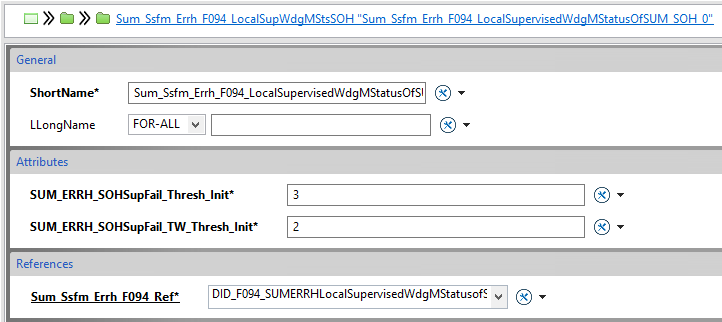
\includegraphics[scale=0.40]{images/F094_config.PNG}
\end{figure}

The Sum\_Ssfm\_LocalSupWdgMStsOfSOHNvmRef parameter in the Sum\_Ssfm\_NvM\_References sub-container shall be configured to refer to the NVM blocks where the DID F094 data stored. 

\begin{figure}[H]
	\centering
	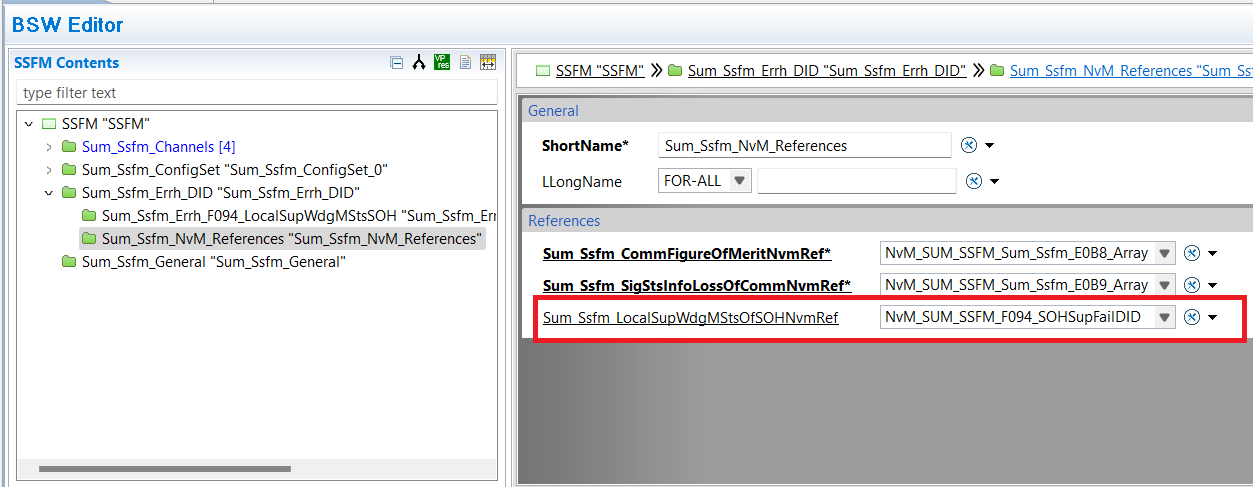
\includegraphics[scale=0.40]{images/NvMBlock_DID_F094_Ref.PNG}
\end{figure}

The Sum\_Ssfm\_LocalSupWdgMStsOfSOHNvmRef shall be configured when the SOH\_ERRHLocalSupervision\_ SupportEnabled is True; otherwise, it does not need to be.
\begin{figure}[H]
	\centering
	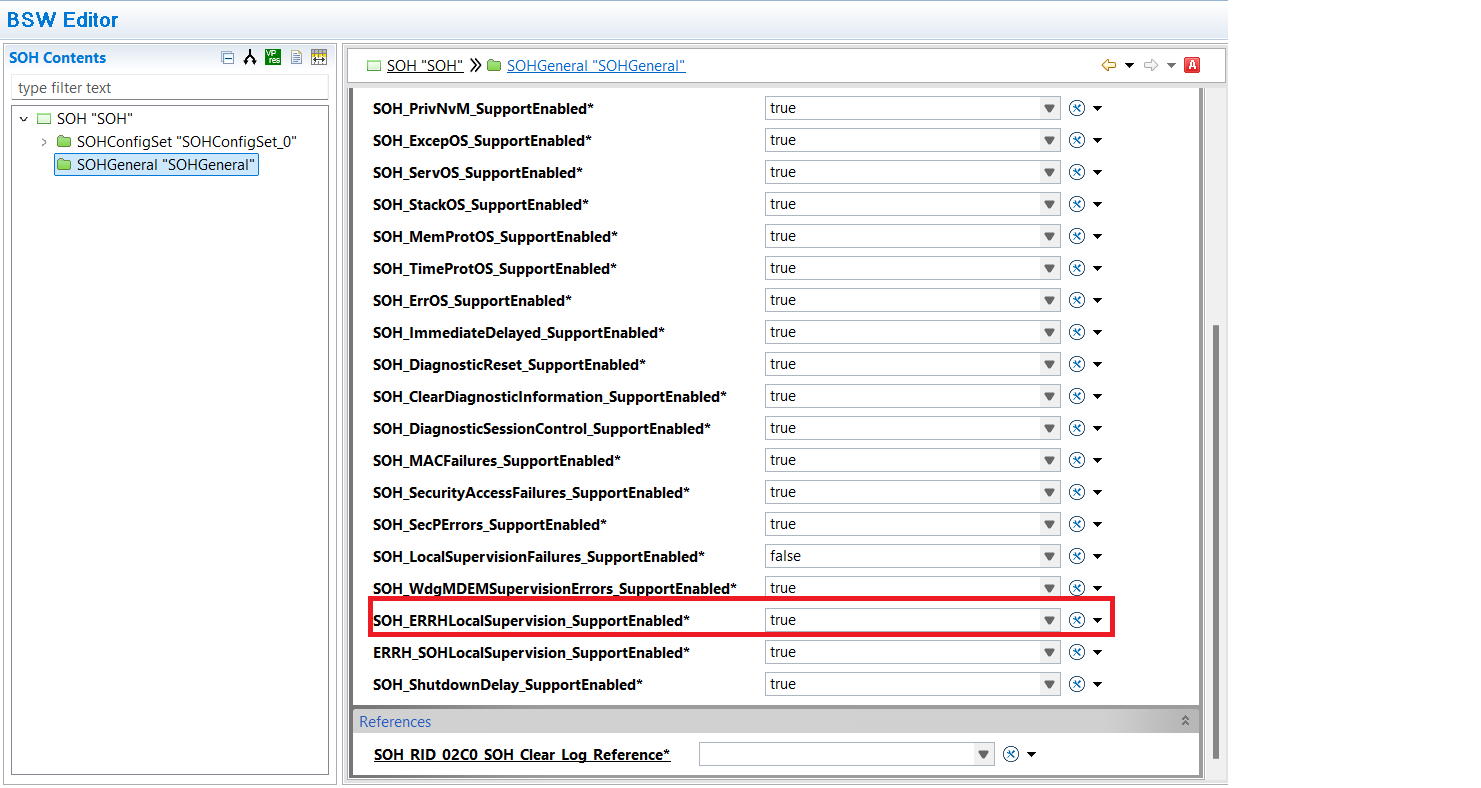
\includegraphics[scale=0.4]{images/LocalSupervision_SupportEnabled.PNG}
\end{figure}

The NvM block for DID 0xF094 will be generated during the Confgen step with the necessary information for SumCode generation.
\begin{figure}[H]
	\centering
	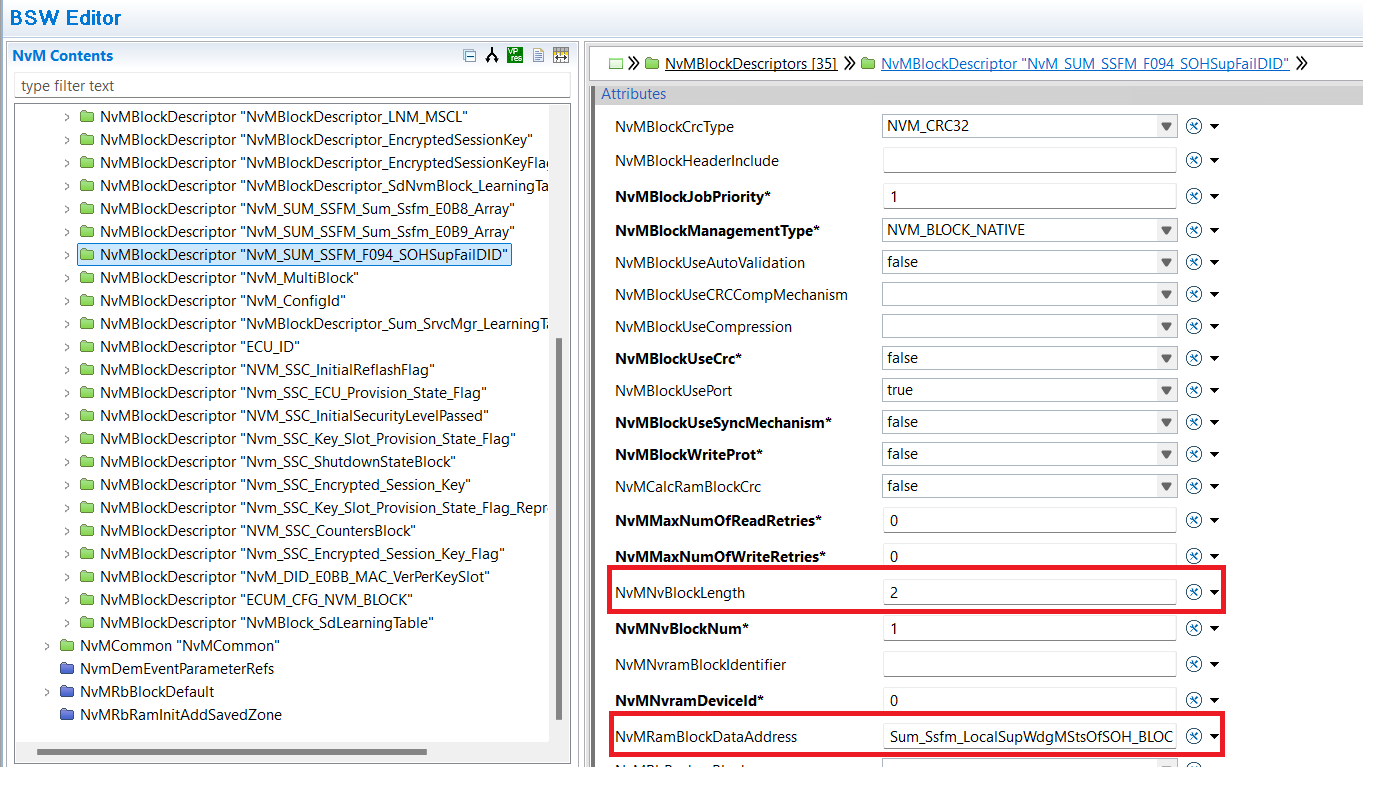
\includegraphics[scale=0.30]{images/NvMBlock_DID_F094.PNG}
\end{figure}

Since the DID data must be saved in non-volatile memory, it is necessary to connect the PS\_NvM\_SUM\newline\_SSFM\_F094\_SOHSupFailDID port of the NvM module to the RP\_ERRH\_NvMSOHSupFailDID port of the SSFM module. Please, 
take into account the fact that the PS\_NvM\_SUM\_SSFM\_F094\_SOHSupFailDID port will be generated after BSW generation subsequently to Confgen step. 

In addition, if the \code{ERRHLocalSupervision\_SupportEnabled} parameter present in the SOH module is set to true, the \code{SUM\_ERRH\_SOHSupFail\_Thresh\_Init} and \code{SUM\_ERRH\_SOHSupFail\_TW\_Thresh\_Init} parameters, within the SSFM module, must be configured in order to take advantage of the proper functioning of this DID feature.

\begin{figure}[H]
	\centering
	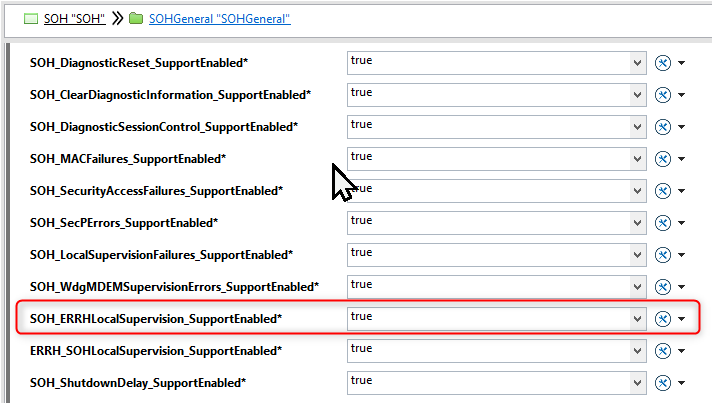
\includegraphics[scale=0.40]{images/F094_SOH_config.PNG}
\end{figure}



\subsection{RID 0x02C0}
\label{subsec:Rid02c0}
RID 0x02C0 is implemented by SUM\_SOH that interacts with DCM for handling such routine. However, SUM\_SOH Local Supervision Detector is implemented by SUM\_SSFM. That is, SUM\_SSFM
is in charge of all operations related to this detector.
Hence, in order to complete the RID 0x02C0 routine, SUM\_SOH shall interact with the SUM\_SSFM through the Client Server interface SOH\_ERRH\_ClearRID0x02C0 where SUM\_SSFM acts as Server.
\newline If SUM\_SOH is \textbf{not integrated}, P-Port \textbf{PP\_SOH\_SSFM\_ERRH\_ClearRID0x02C0} is not generated.

If SUM\_SOH is \textbf{integrated} and SUM\_SOH Local Supervision Detector is \textbf{disabled} as in figure \ref{fig:sohlocsup}, P-Port \textbf{SOH\_ERRH\_ClearRID0x02C0} is not generated.

Please connect SUM\_SSFM P-Port \textbf{PP\_SOH\_SSFM\_ERRH\_ClearRID0x02C0} to the corresponding R-Port of SUM\_SOH.

\begin{figure}[h!]
	\centering
	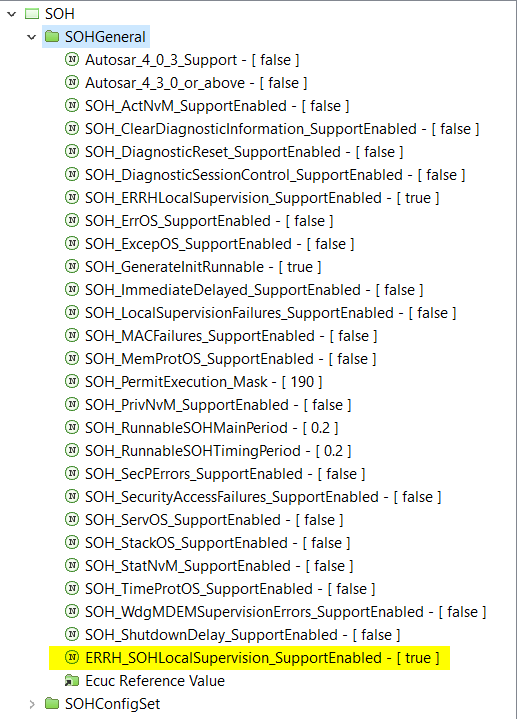
\includegraphics[scale=0.40]{images/sohlocsup}
	\caption{Parameter in SOHGeneral to enable the support DID 0xF094}
	\label{fig:sohlocsup}
\end{figure}


\subsection{BSW Errors Manager}
\label{subsec:BSWErrorsManager}

SSFM-ERRH is set to receive notifications of DEM events for each error via corresponding \\code{DemCallbackEventUdsStatusChanged}. The entity is designed to aggregate all events concerning BSW production errors in the DEM system. 
SSFM-ERRH differentiates between DTC and non-DTC events: DTC events are subject to debouncing, while other events are forwarded to SUM\_SOH. 
For events determined to be DTC relevant, SSFM-ERRH will communicate the associated event to DEM along with its test pass\_fail result.

The BSW Errors Manager is responsible for the following tasks:

\begin{enumerate}
    \item Receive the notifications from a callback of BSW about BSW production error.
	\item Develop the error filter logic to check the conditions and decide whether to set a DTC.
    \item Notify Dem of respective errors based on filtering result.
	\item Notifies SOH of the following BSW errors using the BswEvent (Bitmap uint32):
	\begin{itemize}	
		\item NVM\_E\_HARDWARE
		\item NVM\_E\_INTEGRITY\_FAILED
		\item NVM\_E\_REQ\_FAILED
		\item NVM\_E\_WRONG\_BLOCK\_ID
		\item NVM\_E\_VERIFY\_FAILED
		\item NVM\_E\_LOSS\_OF\_REDUNDANCY
		\item NVM\_E\_QUEUE\_OVERFLOW
		\item NVM\_E\_WRITE\_PROTECTED
		\item WDGM\_E\_SUPERVISION
		\item WDGM\_E\_SET\_MODE
	\end{itemize}
	\item Storing the confirmed Communication Channel BusOff error.
\end{enumerate}

\paragraph{Checking calibration parameter process DTC} 
To control the process of DTC for BSW Errors via reading configured calibration parameter \\Sum\_Ssfm\_Errh\_C\_BswDTCProcess.

\begin{figure}[H]
	\centering
	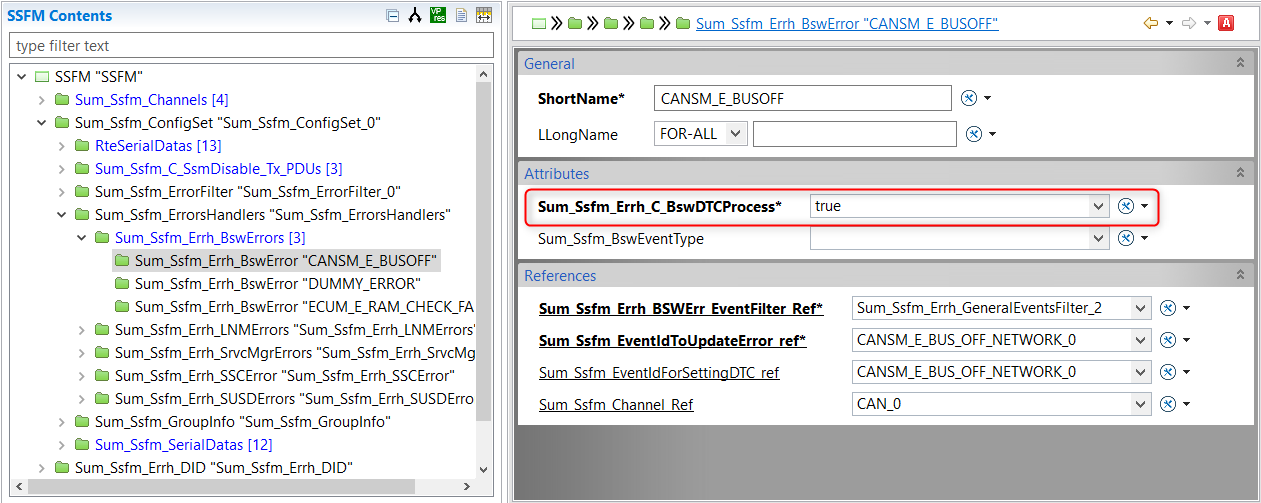
\includegraphics[scale=0.40]{images/BswDTCProcess.PNG}
\end{figure}


\paragraph{Setting the reference to event filter for BSW Errors}
To get the reference to the general event filter, the user should configure the Sum\_Ssfm\_GeneralEventFilter used for associated BSW Errors as the example image below.

Note: Each of the error shall have the invidual instance of Sum\_Ssfm\_GeneralEventFilter. So the user needs to create each instance Sum\_Ssfm\_GeneralEventFilter for each error.

\begin{figure}[H]
	\centering
	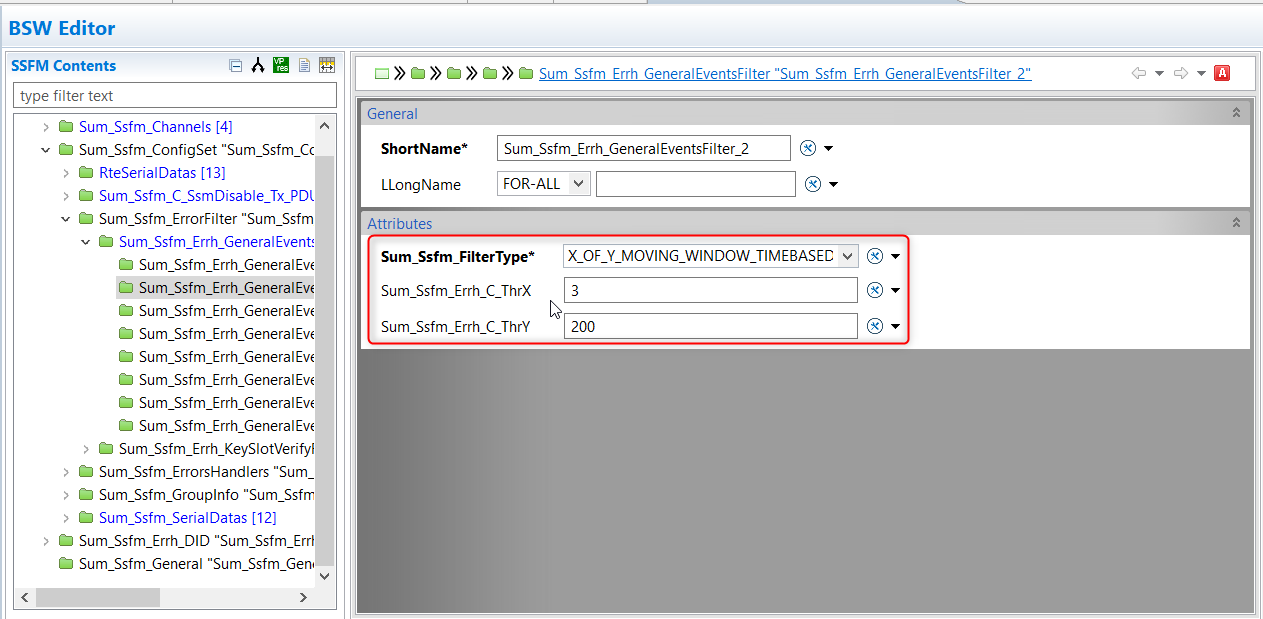
\includegraphics[scale=0.40]{images/BSW_ERROR_GeneralEventFilter.PNG}
\end{figure}

\begin{figure}[H]
	\centering
	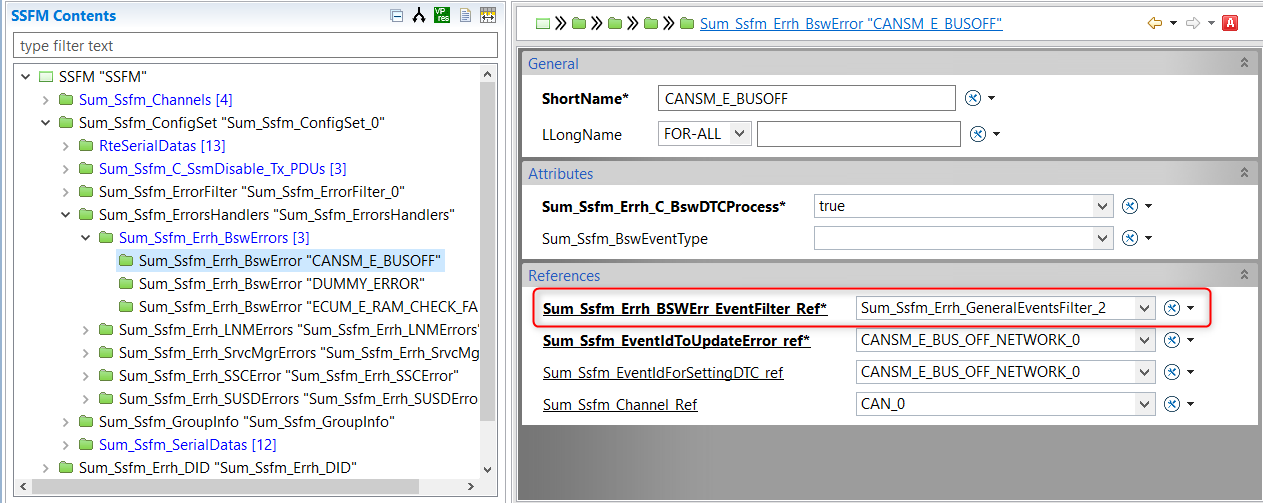
\includegraphics[scale=0.40]{images/BSW_ERROR_EVENT_REF.PNG}
\end{figure}


\paragraph{Setting the Reference to the associated DEM event for filtering}
Users must configure the \\Sum\_Ssfm\_EventIdToUpdateError\_ref parameter with associated DTC for each error in order to Check error debouncing.

\begin{figure}[H]
	\centering
	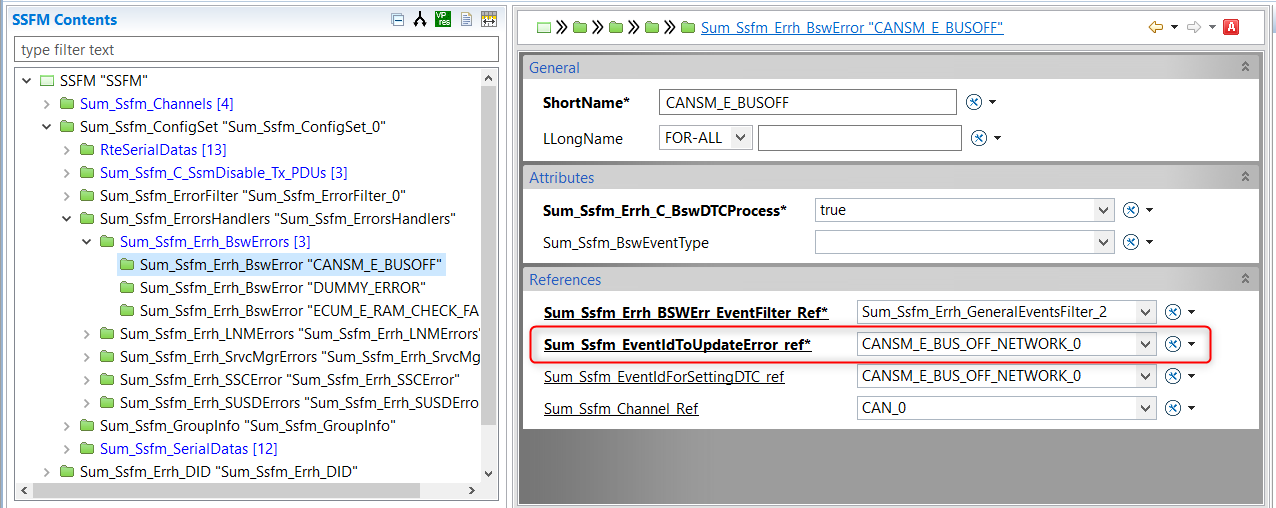
\includegraphics[scale=0.40]{images/EventIdToUpdateError.PNG}
\end{figure}

Note: It is assumed, Reference events are configured in the DEM module for the specific BSW error.
Here this reference is used to get the DTC of associate BSW Errors.


\paragraph{Reference for the associated DEM event that sets the DTC for this relevant error}
User should configure the Sum\_Ssfm\_EventIdForSettingDTC\_ref for each DTC relevant error to set the DTC when a debounced error is confirmed.

\begin{figure}[H]
	\centering
	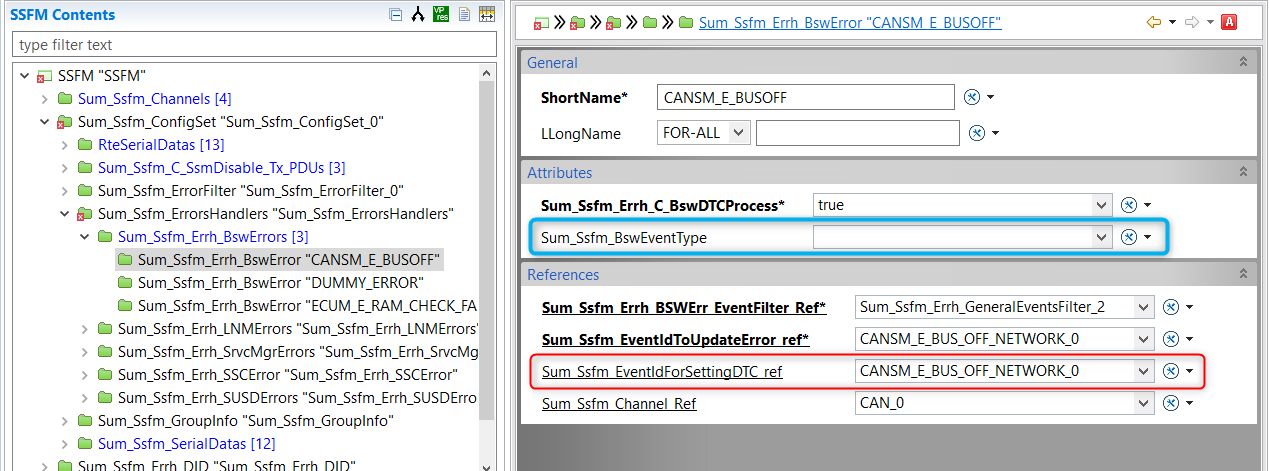
\includegraphics[scale=0.40]{images/EventIdForSettingDTC.PNG}
\end{figure}

Note: It is assumed, the events are DTC relevant and configured in the DEM module. 
If its not DTC relevant then Sum\_Ssfm\_BswEventType must be configured.
Here this reference is used to set/reset dem events based on filtering result.


\paragraph{Selecting BSW error Type to Notify SOH}
User should configure Sum\_Ssfm\_BswEventType by selecting the Event type of error so error can be notified to SOH.
The ERRH\_E\_BswEvent interface is represented as a bitmap of uint32, and the below image provides information on the corresponding bitfields for various errors.

\begin{figure}[H]
	\centering
	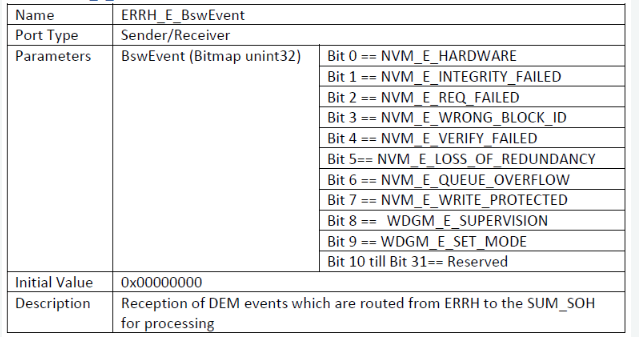
\includegraphics[scale=0.50]{images/BswError_NotifySOHInfo.PNG}
\end{figure}

Note: It is assumed that error is not DTC relevant. 
If its DTC relevant then Sum\_Ssfm\_EventIdForSettingDTC\_ref must be configured.

\begin{figure}[H]
	\centering
	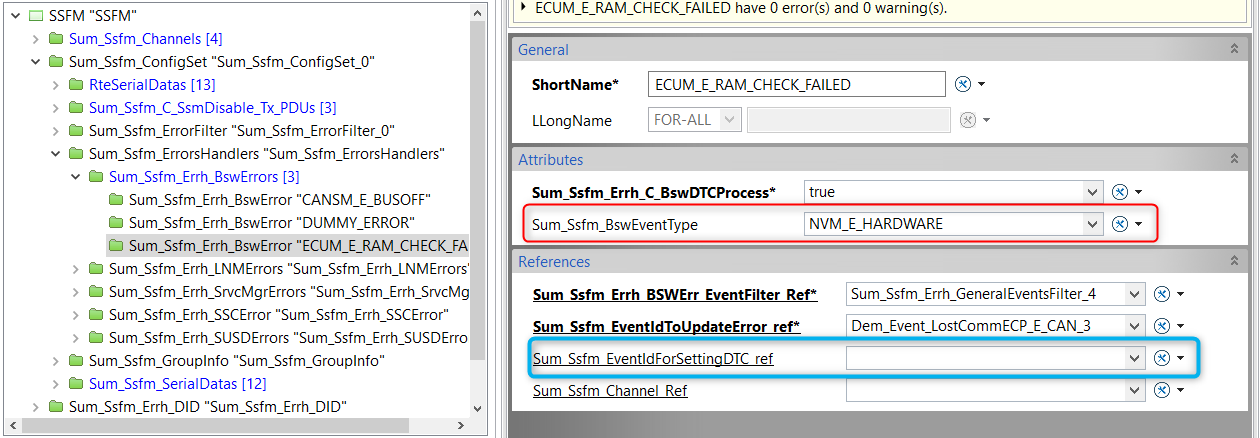
\includegraphics[scale=0.40]{images/BswError_NotifySOH.PNG}
\end{figure}

Note: Select corresponding event type for error. example if error is NVM\_E\_REQ\_FAILED the select NVM\_E\_REQ\_FAILED event only.

\paragraph{Setting the Reference to COM channel for BSW Error}
To get the reference to Communication channel if error type is CAN or ETH BUS\_OFF. \\Sum\_Ssfm\_Channel\_Ref.

\begin{figure}[H]
	\centering
	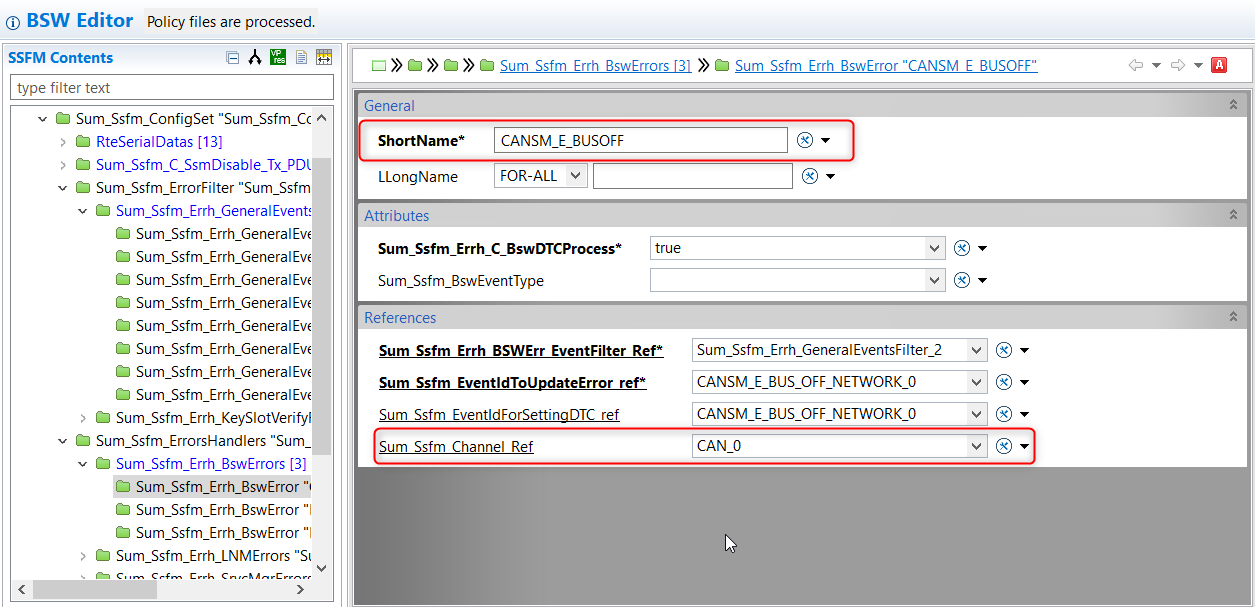
\includegraphics[scale=0.40]{images/BswError_ChannelRef.PNG}
\end{figure}

Note: Select Channel ref only if error type is communication BusOff.

\newpage
\subsection{Sum SSFM Local Supervision}
\label{subsec:SumSSFMLocalSupervision}

Sum SSFM needs to be supervised by the WdgM, so that SOH can check its status for the DID 0xF093. The communication between the submodule Errh and Wdgm is allowed by using the interface WdgM\_LocalSupervision.
To establish this communication, the user must:
\begin{enumerate}
    \item create the WdgM module, including the WdgIf and the Wdg driver;
    \item configure the Sum SSFM as a Supervised Entity within the WdgM;
    \item configure an Alive Supervision that references the checkpoint SSFM Errh;
    \item configure the parameters in the Alive Supervision accordingly to the periodicity of the \\ Runnable\_SSFM\_ExecutionManager (Sum\_Ssfm\_ExecutionManagerPeriodicity parameter);
	\item configure the parameter Sum\_Ssfm\_Soh\_General\_Ref within the SSFM module, referencing the SOH module;
	\item set to True the parameter SOH\_ERRHLocalSupervision\_SupportEnabled within the SOH module;
	\item generate the BSW code;
	\item connect the port of SSFM RP\_SSFM\_ERRH\_WdgM\_WdgM\_LocalSupervision with that of the WdgM (interface WdgM\_LocalSupervision);
	\item generate the RTE code.
	
\end{enumerate}

\subsection{LIN Responder Error Manager}
\label{subsec:LINRespErrorManager}

\paragraph{Prerequisites}
SUM\_LNM must be available beforehand, as SSFM requires the configuration in SUM\_LNM for interaction between the two modules.

\paragraph{Setting parameter Sum\_Ssfm\_LINInfo:}
\begin{enumerate}
    \item Refer to ~\ref{par:lininfogroup} to configure the \texttt{Sum\_Ssfm\_LINInfo} parameter.
	\item Configure \texttt{Sum\_Ssfm\_LINResponderOBD\_Supported} for each of LIN Responder to determine \\ whether OBD is supported by LIN Responder.
\end{enumerate}

\begin{center}
	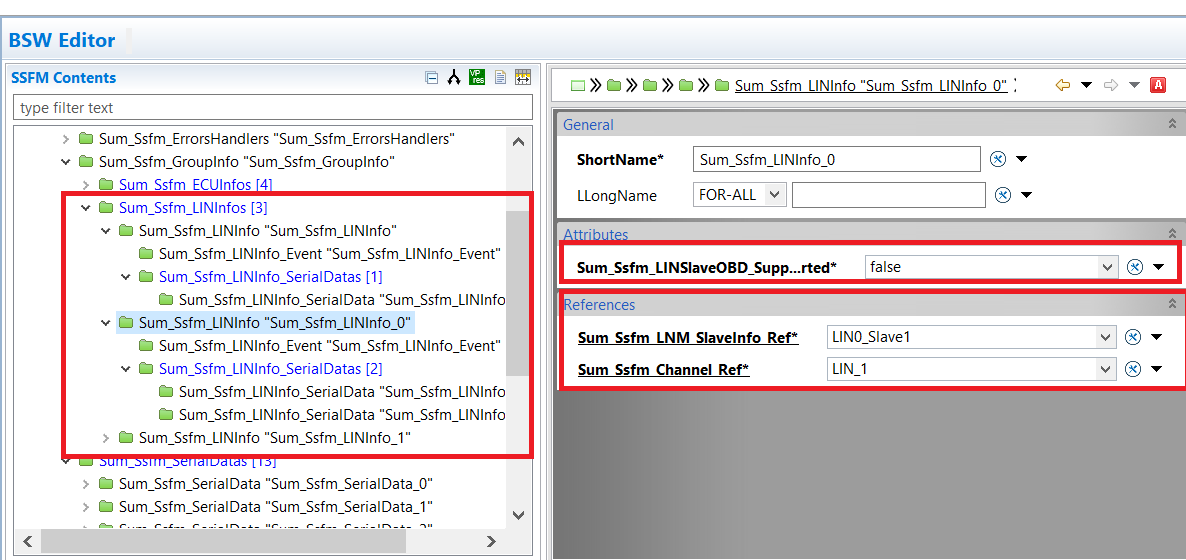
\includegraphics[width=0.7\textwidth]{images/LINInfo}
\end{center}

\paragraph{Creating instance for Sum\_Ssfm\_LNM\_ResponderInfoError:}
The user shall create the an instance for each of LIN Responder in container \texttt{Sum\_Ssfm\_Errh\_LNMErrors}:
\begin{enumerate}
	\item Select the debouncing filter instance \texttt{Sum\_Ssfm\_LNMResponderErr\_EventFilter\_Ref}, which is referenced to \texttt{Sum\_Ssfm\_Errh\_GeneralEventsFilter}.
    \item Select the reference to \texttt{Sum\_Ssfm\_LINInfo\_Ref} associated with a LIN Responder.
\end{enumerate}

\begin{center}
	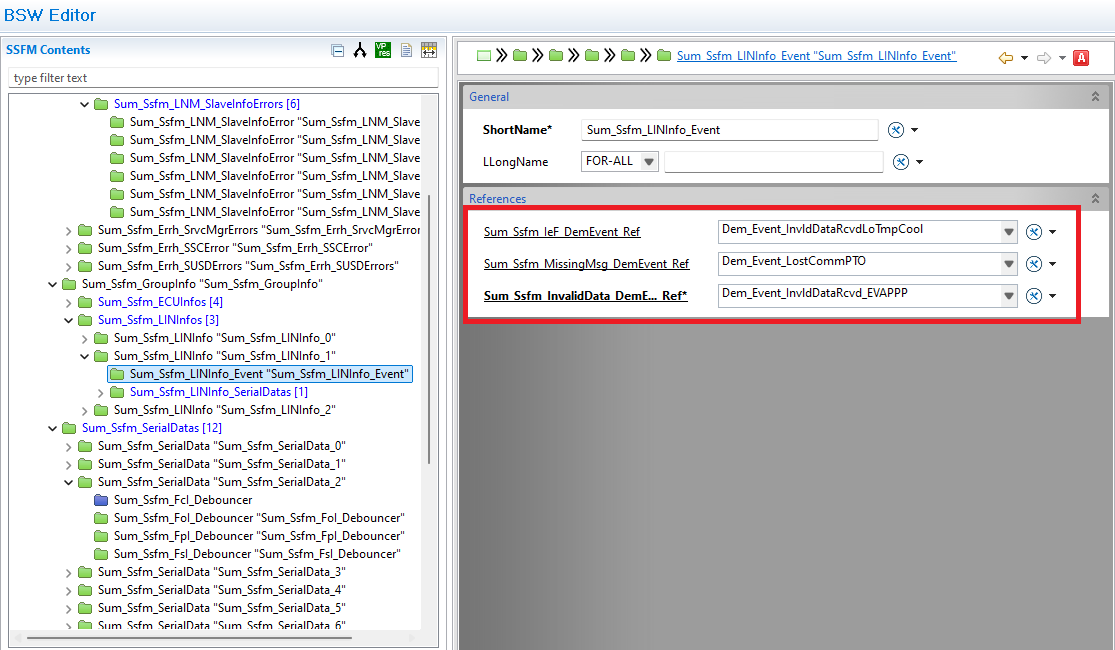
\includegraphics[width=0.7\textwidth]{images/LINInfo_Events}
\end{center}

\begin{center}
	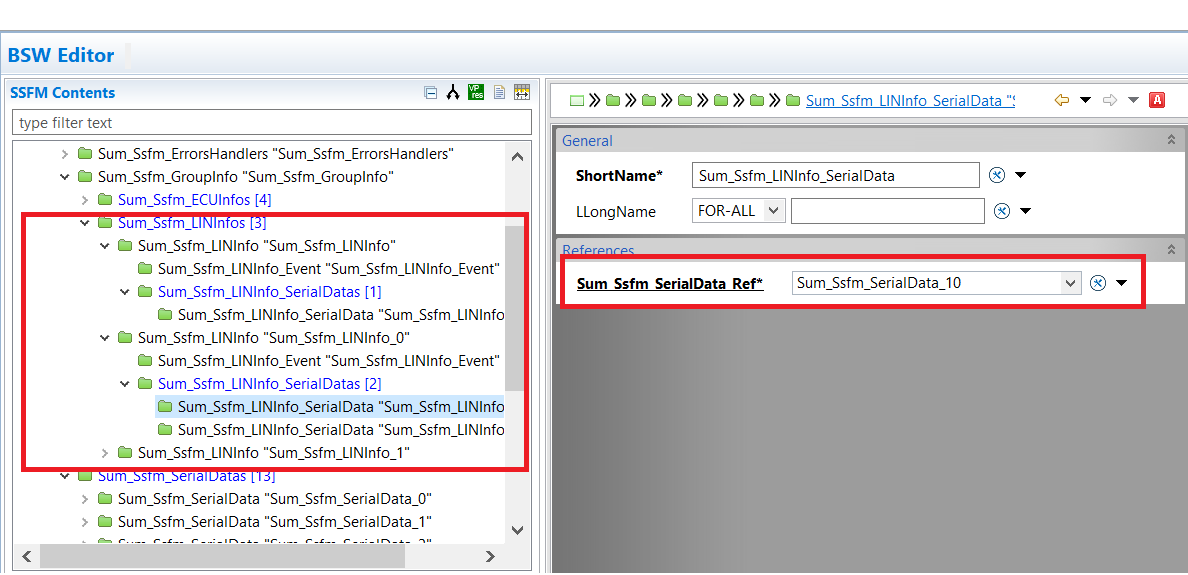
\includegraphics[width=0.7\textwidth]{images/LINInfo_SerialDatas}
\end{center}

\paragraph{BatteryVoltageRangeMinToMax interface}
The R-Port related to the interface \texttt{BatteryVoltageRangeMinToMax} shall be connected to \\SUM\_SUSD. In Sum\_SUSD the container SUSD\_Battery\_Voltage\_Supported shall be enabled and the minimum and maximum voltage shall be defined. 
SUM\_SSFM shall receive battery voltage level using this port.

\subsubsection{LIN Responder Internal Electronic Fault}
\label{subsubsec:LINRespIeFManager}

To use the functionality for invalidating a LIN signal, the user shall perform the following steps:
\paragraph{Setting parameter Sum\_Ssfm\_LINInfo:}
The user shall set the \texttt{Sum\_Ssfm\_IeF\_DemEvent\_Ref} parameter to the Dem event that tracks the Internal Electronic Fault data events for the referenced LIN Responder.

\paragraph{Creating instance for Sum\_Ssfm\_LNM\_ResponderInfoError:}
The user shall select \texttt{Sum\_Ssfm\_LNM\_ResponderInfoErrorType} as SSFM\_LNM\_RESPONDER\_IEF to indicate the error type is an Internal Electronic Fault.

\paragraph{SSFM\_LIN\_Signal\_Inv and LNM\_ERRH\_IntElectFault interface}
To properly notify the invalidity of a LIN signal, it is necessary to connect the SSFM\_LIN\_Signal\_Inv<n> to the SWC and the LNM\_ERRH\_IntElectFault<X> interface to the SUM\_LNM.

\paragraph{Setting Dem Callback DTC Status Changed}
The user shall also configure a \texttt{DemCallbackDTCStatusChanged} instance under the Dem General Configuration 
with a callback function named as \texttt{Ssfm\_Dem\_CB\_DTCStatusChanged} to enable the DTC setting feature.

\subsubsection{LIN Responder Missing Message}
\label{subsubsec:LINRespMissingMsg}

To use the functionality for missing message of the corresponsding LIN Responder, the user shall:
\begin{enumerate}
	\item Set \texttt{Sum\_Ssfm\_MissingMsg\_DemEvent\_Ref} parameter to the Dem event that tracks the Missing Message Failure data events for the referenced LIN Responder.
	\item Select \texttt{Sum\_Ssfm\_LNM\_ResponderInfoErrorType} as SSFM\_LNM\_RESPONDER\_MISSING\_MSG to indicate the error type is a Missing Message Failure.
\end{enumerate}

\paragraph{Configuring Calibratable Time}
To properly handle the test enablement for the LIN Responder missing message failure, the user shall configure the calibratable time \texttt{Sum\_Ssfm\_MissingMsg\_CalibratableTime} (in seconds).

\paragraph{Configuring Periodicity of the Function}
To properly execute the internal logic of the function to check for the test enable condition for a missing message error, the user shall configure the periodicity \texttt{Sum\_Ssfm\_MissingMsg\_Periodicity} (in milliseconds).

\begin{center}
	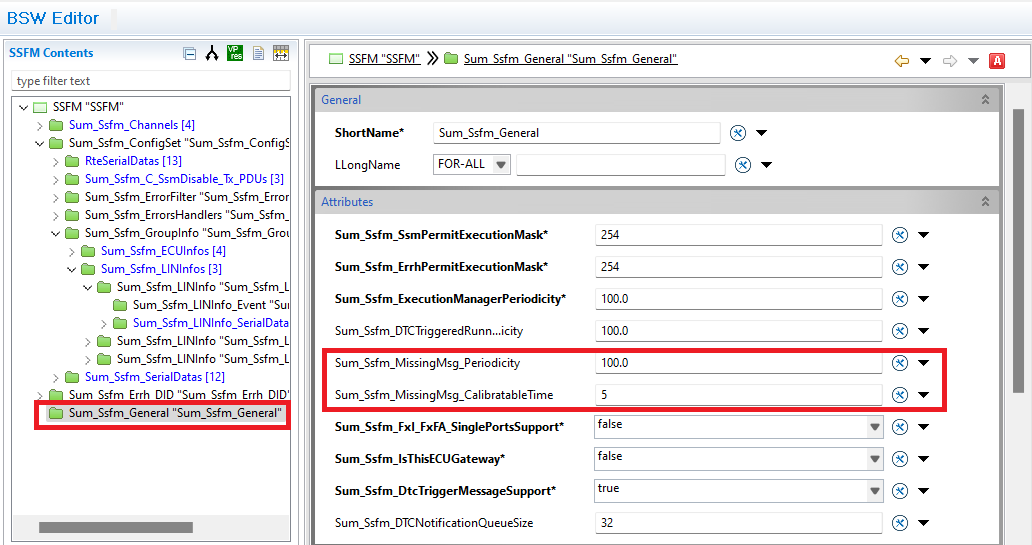
\includegraphics[width=0.7\textwidth]{images/LINInfo_MissingMessage_General}
\end{center}

\paragraph{LNM\_ERRH\_NodeStatusId interface}
To properly getting notification from SUM\_LNM of the error status of the associated code of each LIN Responder, it is necessary to connect the LNM\_ERRH\_NodeStatusId<n> to the SUM\_LNM.

\paragraph{SSM\_LNM\_NodeTimeout interface}
To properly notifying the node timeout status of the associated of each LIN Responder, it is necessary to connect the SSM\_LNM\_NodeTimeout<n> to the SUM\_LNM.

\subsection{LIN Availability Status Manager}
\label{subsec:LINAvStsManager}

\paragraph{Prerequisites}
SUM\_LNM must be available beforehand, as SSFM requires the configuration in SUM\_LNM for interaction between the two modules.
The following actions have to be done to enable the LIN availability status:

\paragraph{Configure LIN SerialDatas}
In order to enable SSFM to determine the availability status of the LIN SerialDatas, all LIN SerialDatas
has to be defined as \textbf{Sum\_Ssfm\_SerialData} container with a valid Channel Reference to a LIN Channel.

\paragraph{Connect the LNM\_SSM\_MSCL\_LIN interface}
The P-Port of LNM \textbf{LNM\_SSM\_MSCL\_LIN} has to be connected to SSFM to determine the MSCL status required for disable condition assessment.

\paragraph{Connect the LNM\_SSM\_MSCL\_LIN interface}
The P-Port of BswM \textbf{LinSM\_CurrentSchedule} has to be connected to SSFM to determine the LIN schedule status required for disable condition assessment.

\subsection{DTCTriggered Message Generator Handler}
\label{subsec:DTCTriggeredMessage}

DTCTriggered Message Generator Handler is responsible for the following tasks:

\begin{enumerate}
    \item Get a DTC when there is a change in the status ( EventStatusChanged) then put it in the queue.
	\item Checks if at least one Partial Network Cluster (PNC) is active to ensure communication is active.
	\item Sends the DTC triggered message if the wait timer exceeds 1000ms or during the initial power-up sequence.
	\item Dequeues DTCs from the notification queue and updates the DTC triggered message fields if the wait timer exceeds 1500ms.
	\item Manages internal timers to control the periodicity of message sending and DTC status updates. 
\end{enumerate}

\paragraph{Checking calibration parameter process DTC} 
To control this function via a parameter (Sum\_Ssfm\_DtcTriggerMessageSupport). 
When it's select TRUE value, all the functions related to the DTC Triggered Message generated.

\begin{figure}[H]
	\centering
	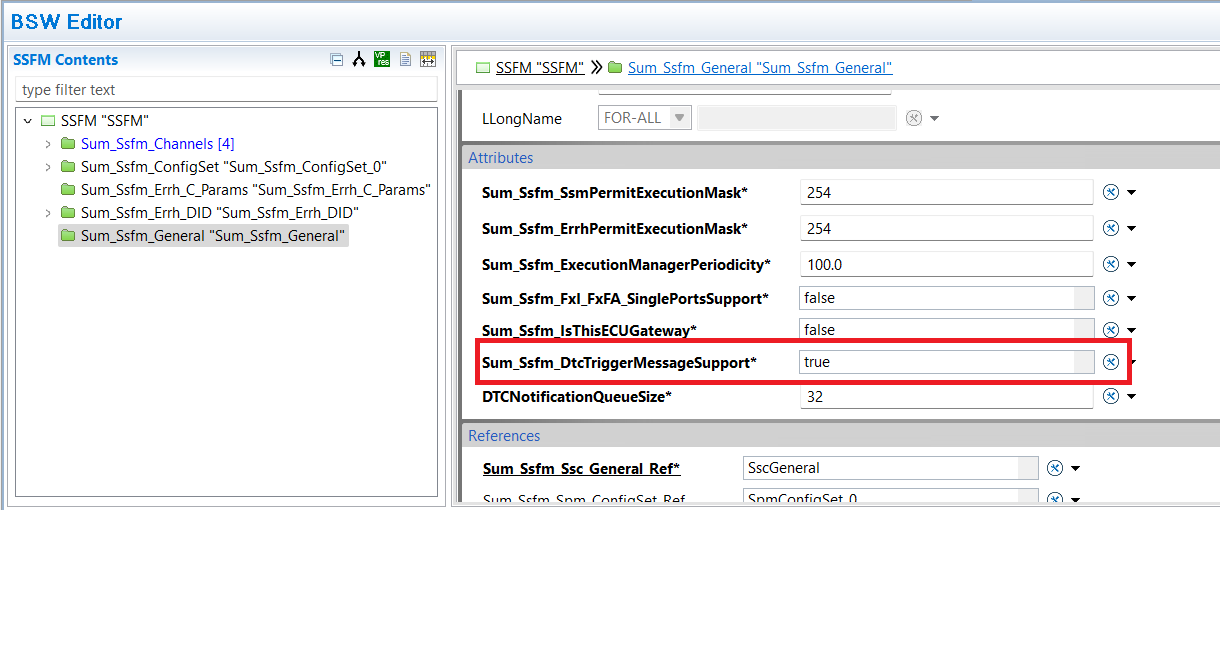
\includegraphics[scale=0.40]{images/Sum_Ssfm_DtcTriggerMessageSupport.png}
\end{figure}


\paragraph{Setting the size of Queue}
To set the size of queue, the user should configure the (Sum\_Ssfm\_DTCNotificationQueueSize).

\begin{figure}[H]
	\centering
	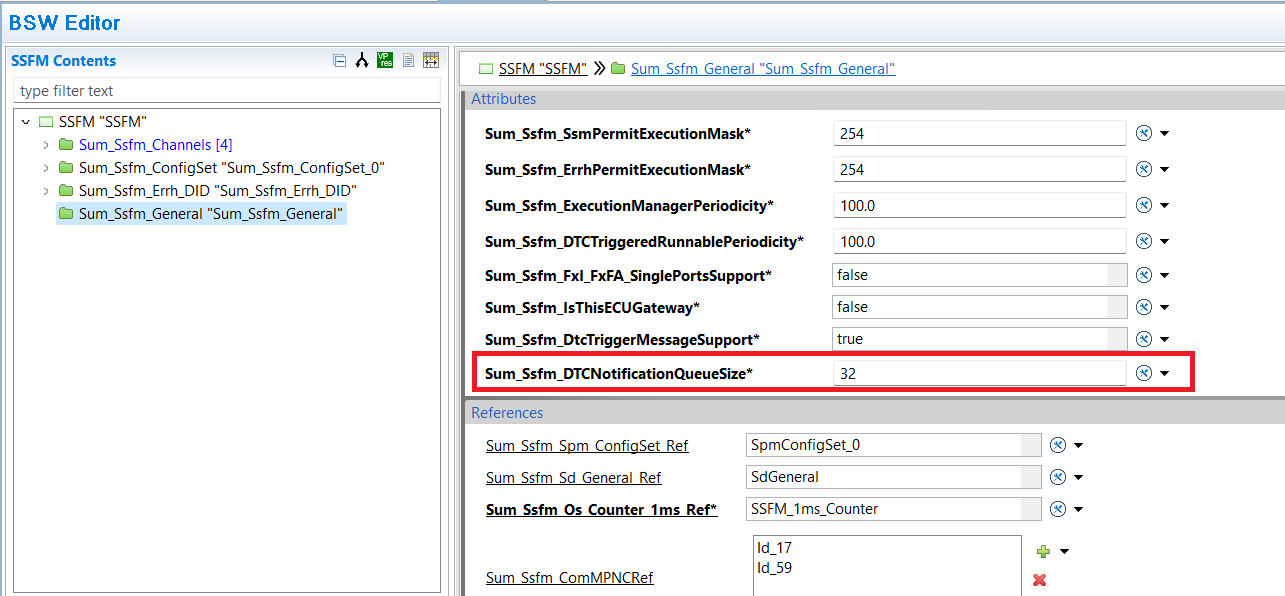
\includegraphics[scale=0.40]{images/dtcNotificationQueueSize.png}
\end{figure}

\paragraph{Setting the Period of Runnable DTCTriggeredMessageHandler}
To set the period of {Runnable\_SSFM\_DTCTriggeredMessage\_Handler}, the user must configure the (Sum\_Ssfm\_DTCTriggeredRunnablePeriodicity) parameter

\begin{figure}[H]
	\centering
	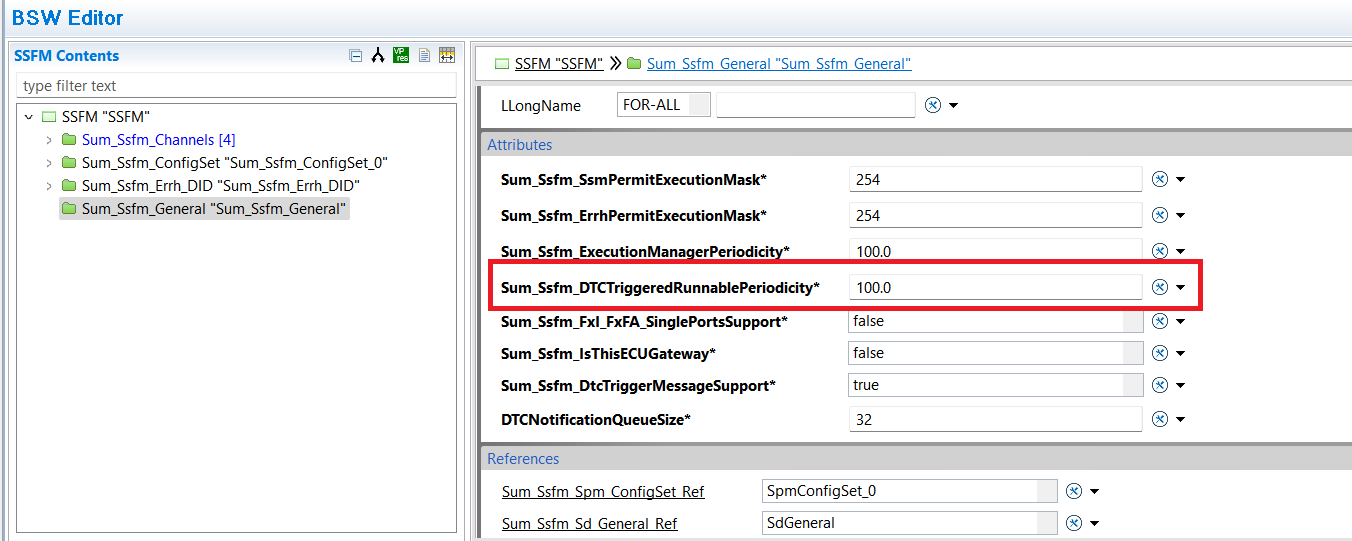
\includegraphics[scale=0.40]{images/PeriodRunnableDTCTrigger.png}
\end{figure}

\paragraph{Configuration of ComMRef for DTC Trigger Message Support}
When {Sum\_Ssfm\_DtcTriggerMessageSupport} is set to enable DTC Trigger Message functionality, the user must configure the {Sum\_Ssfm\_ComMPNCRef} parameter to define all the necessary channels for transmission (TX). This configuration specifies the reference to the Communication Manager Partial Network Cluster (ComM PNC) that the system will use to manage the transmission of DTC messages.

If the user does not configure the {Sum\_Ssfm\_ComMPNCRef} parameter, it indicates that
no Partial Network Cluster Tx (PNCTx) channels are enabled, and therefore, no DTC Trigger Messages will be sent over the network.

\begin{figure}[H]
	\centering
	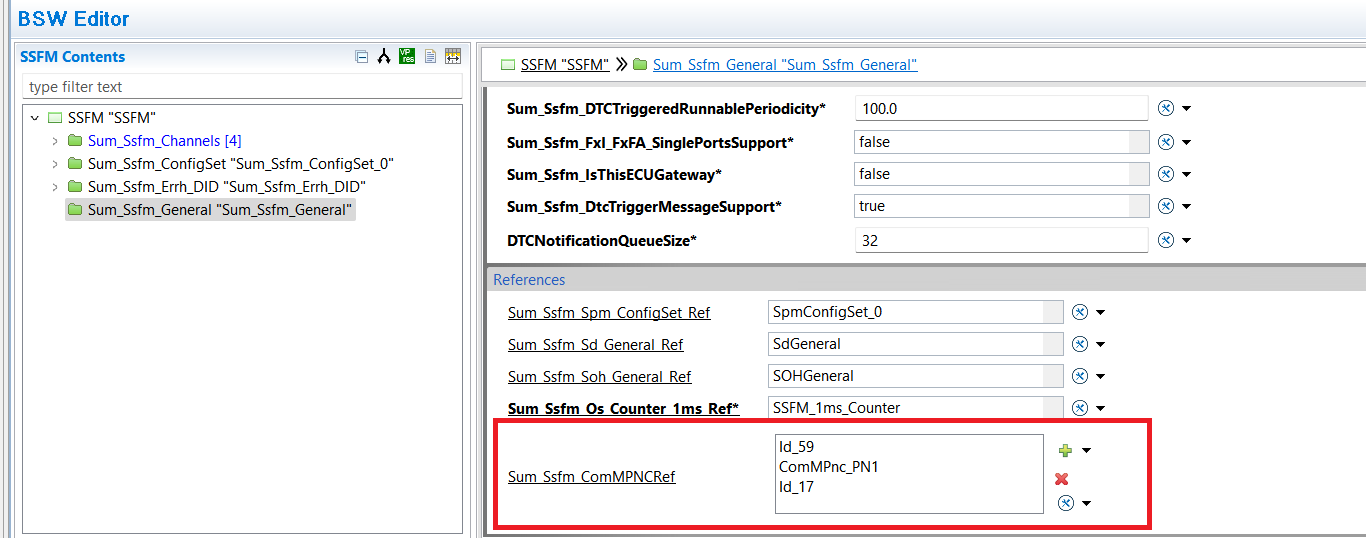
\includegraphics[scale=0.40]{images/ComMRef.png}
\end{figure}

\paragraph{Setting Dem Callback DTC Status Changed}
The user shall also configure a DemCallbackDTCStatusChanged instance under the Dem General Configuration with a callback function named as {Ssfm\_Dem\_CB\_DTCStatusChanged} to enable the DTC setting feature.

\subsection{Dtc Enable Manager}
\label{subsec:DtcEnableManager}

The Dtc Enable Manager is responsible for receiving the DTCs status, utilizing service ControlDTCSetting
0x85, and transmitting this information to the SWCs via the port interface.
To receive the DTCs status, the SSFM module must communicate with the BswM by using the SUM\_ControlDTCSetting port interface. 
To establish this communication, the user must:
\begin{enumerate}
    \item Set to true the attribute DcmSupportDTCSettingControlOptionRecord present under DcmDsp container;
	\begin{figure}[H]
		\centering
		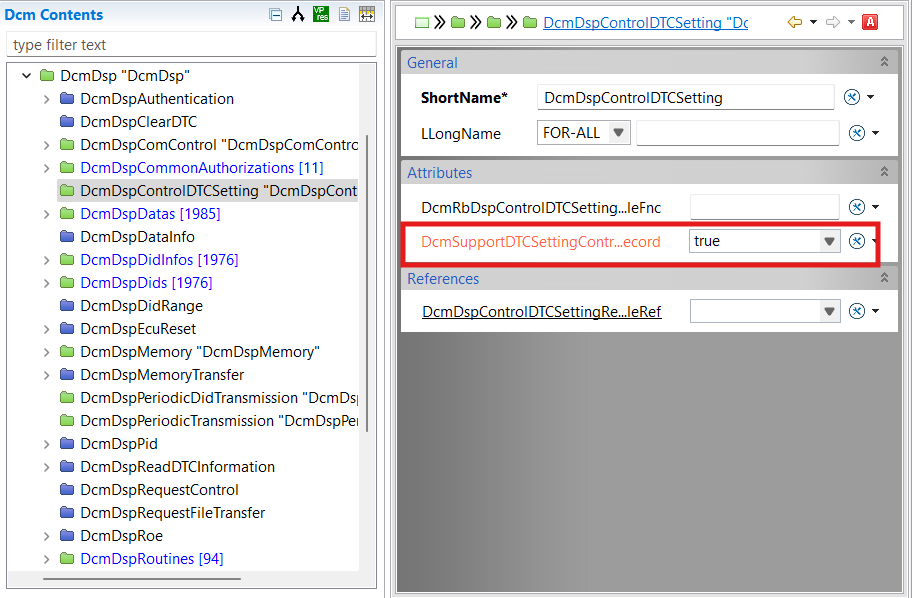
\includegraphics[scale=0.45]{images/Service0x85_0.png}
	\end{figure}
	\item Configure the container ControlDTCSettingClass under the DcmDsdServices;
	\begin{figure}[H]
		\centering
		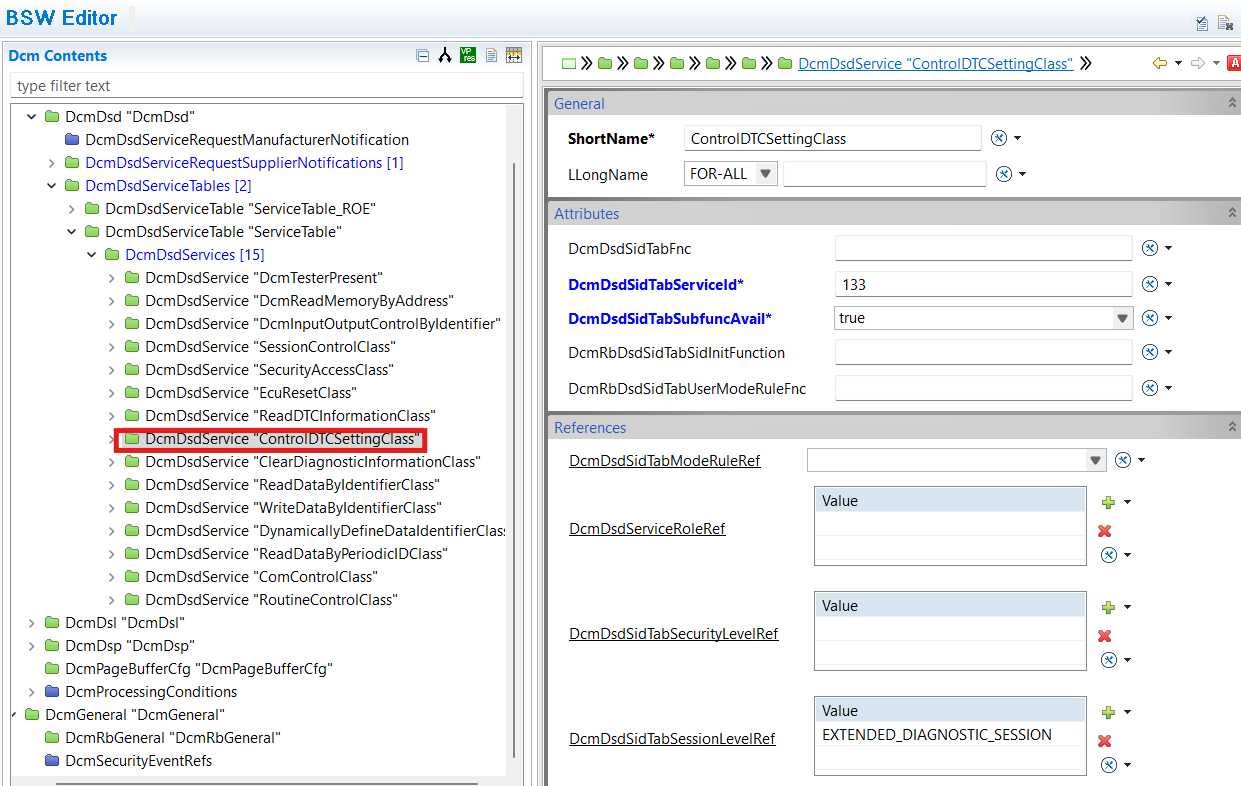
\includegraphics[scale=0.40]{images/Service0x85_1.png}
	\end{figure}
	\item Configure the following containers that are present in the BswM: 
	\begin{figure}[H]
		\centering
		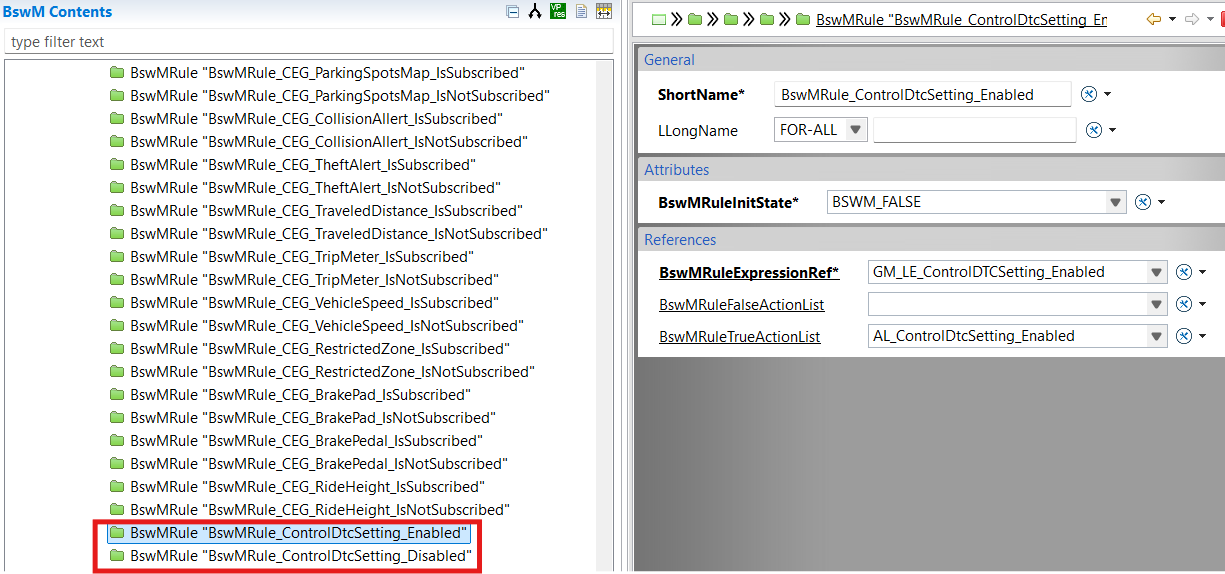
\includegraphics[scale=0.40]{images/BswmCfgService85_1.png}
		\caption{BswMRule}
	\end{figure}
	\begin{figure}[H]
		\centering
		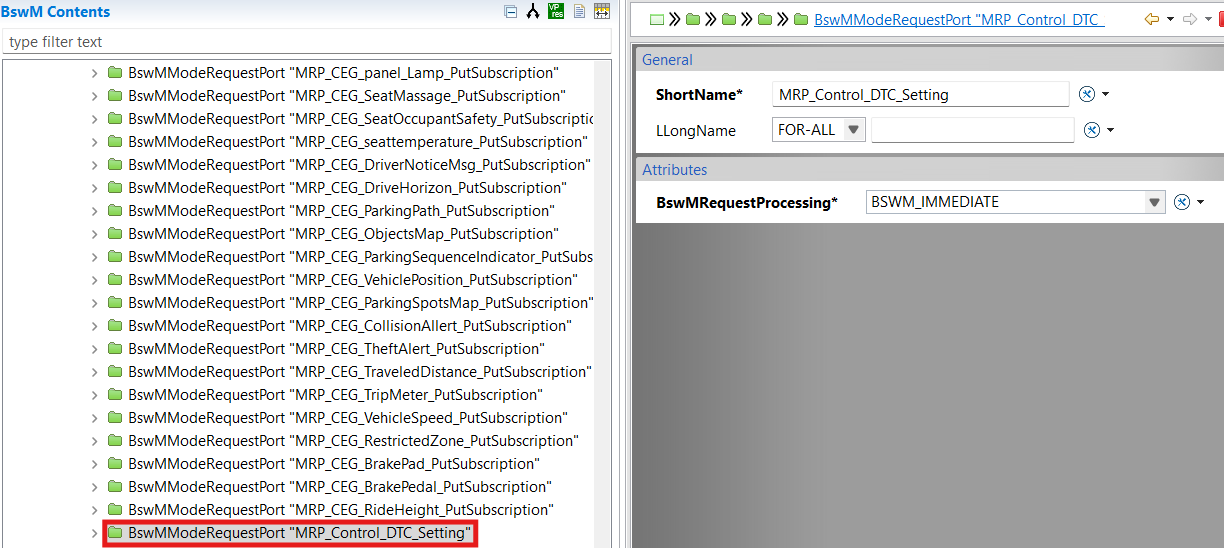
\includegraphics[scale=0.40]{images/BswmCfgService85_2.png}
		\caption{BswMModeRequestPort}
	\end{figure}
	\begin{figure}[H]
		\centering
		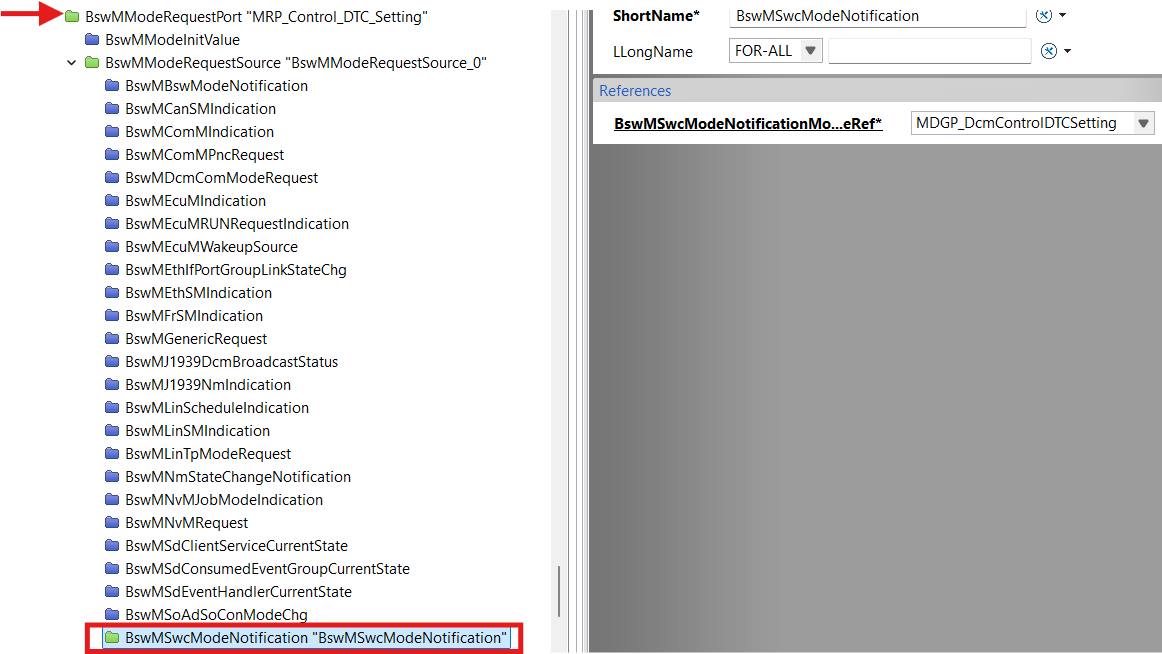
\includegraphics[scale=0.40]{images/BswmCfgService85_2_1.png}
		\caption{BswMSwcModeNotification present under the container BswMModeRequestPort}
	\end{figure}
	\begin{figure}[H]
		\centering
		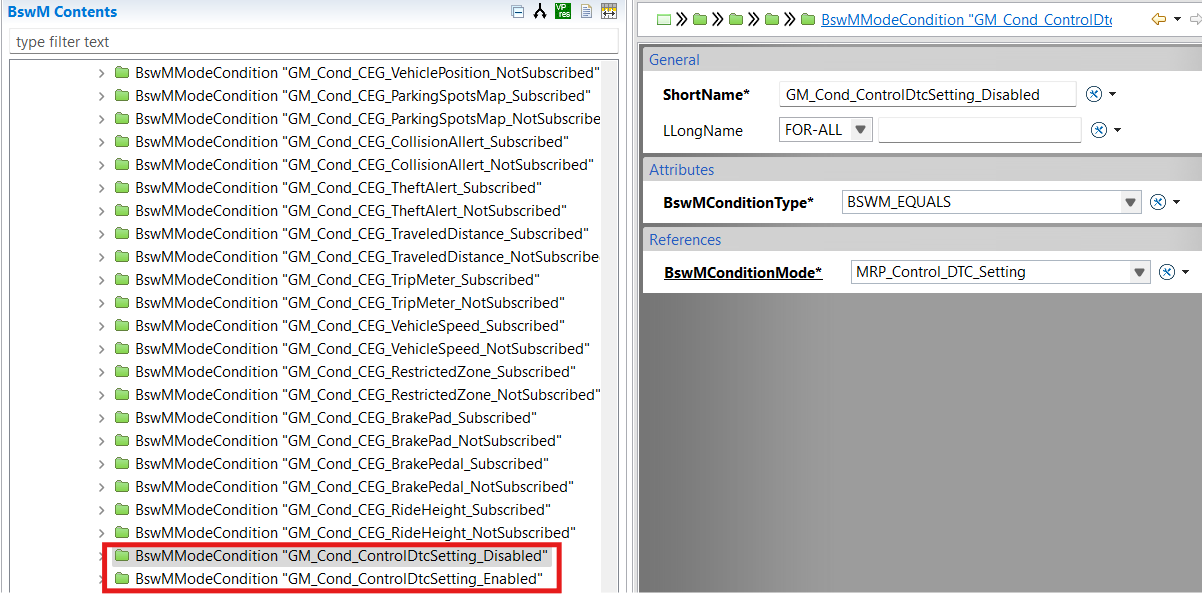
\includegraphics[scale=0.40]{images/BswmCfgService85_3.png}
		\caption{BswMModeCondition}
	\end{figure}
	\begin{figure}[H]
		\centering
		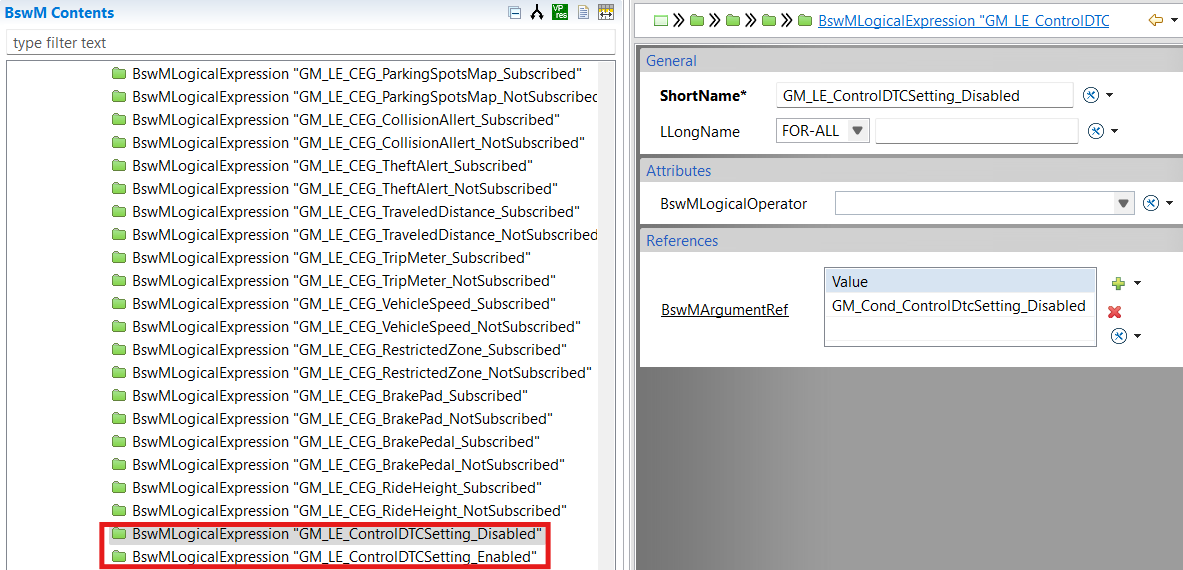
\includegraphics[scale=0.40]{images/BswmCfgService85_4.png}
		\caption{BswMLogicalExpression}
	\end{figure}
	\begin{figure}[H]
		\centering
		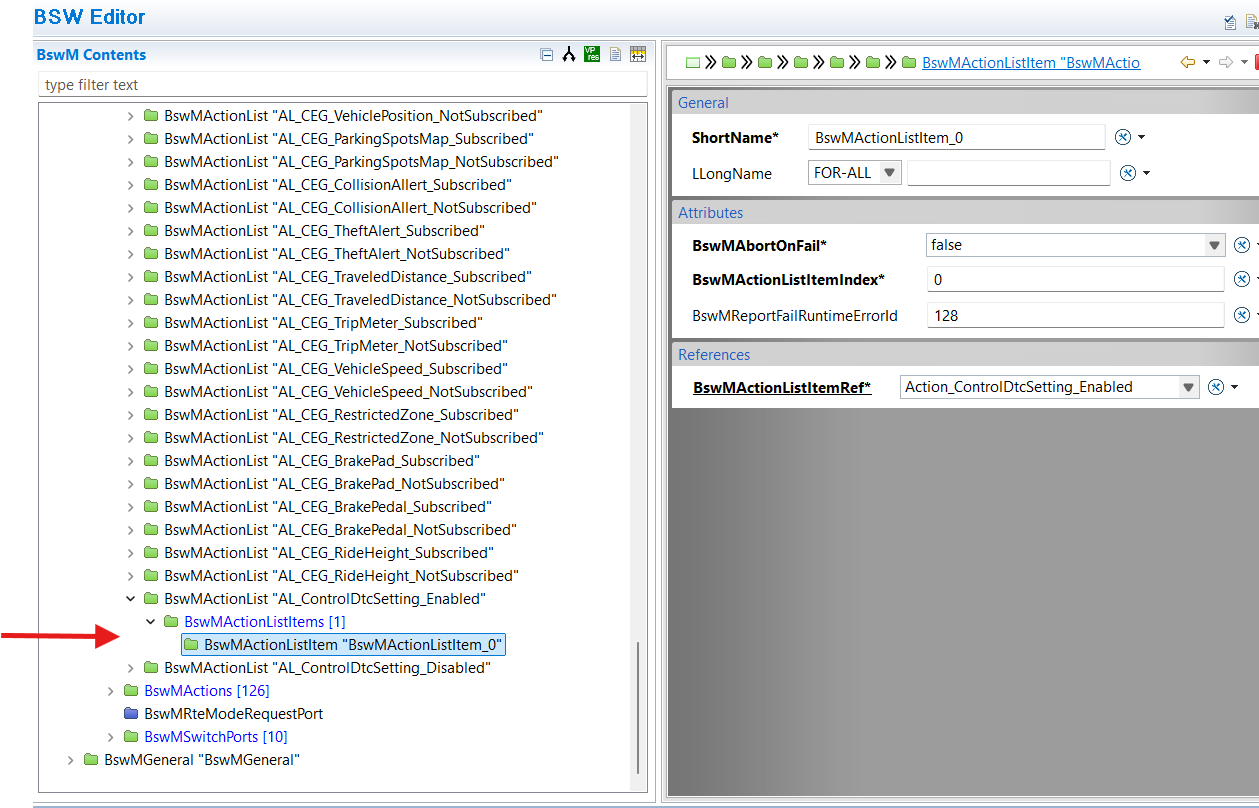
\includegraphics[scale=0.40]{images/BswmCfgService85_5.png}
		\caption{BswMActionListItem present under the container BswMActionList}
	\end{figure}
	\begin{figure}[H]
		\centering
		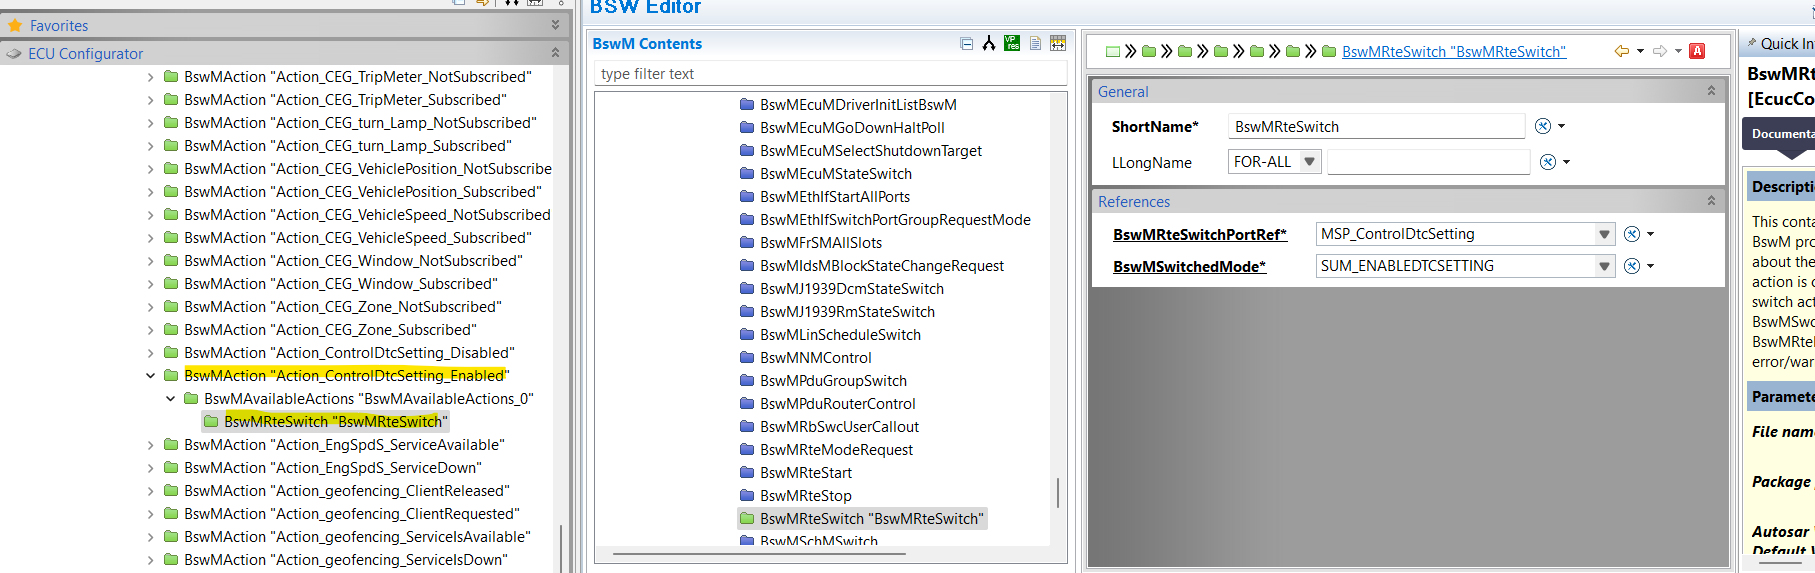
\includegraphics[scale=0.40]{images/BswmCfgService85_6.png}
		\caption{BswMRteSwitch container present under the container BswMAction}
	\end{figure}
	\begin{figure}[H]
		\centering
		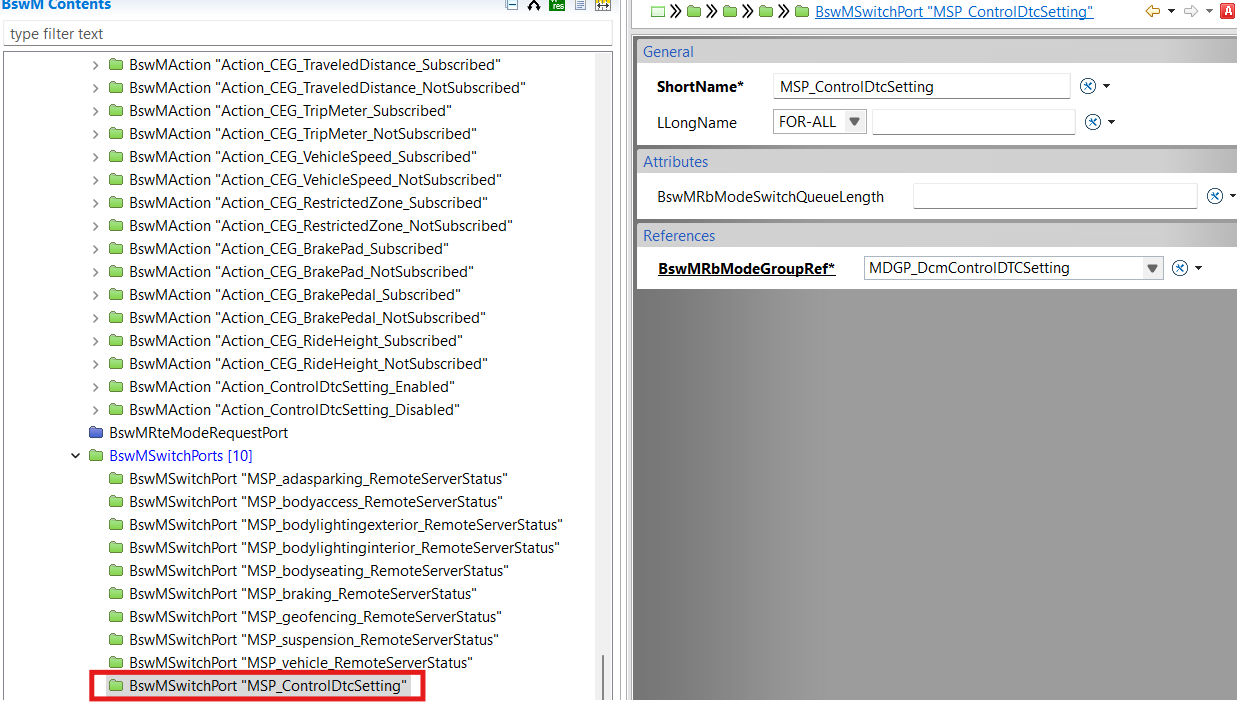
\includegraphics[scale=0.40]{images/BswmCfgService85_7.png}
		\caption{ BswMSwitchPort}
	\end{figure}
	\item Generate the BSW code to obtain the SUM\_ControlDTCSetting mode switch port interface;
	\item Connect the port RP\_ERRH\_BswM\_DisableDTCSetting with that provided by the BswM \\(SUM\_ControlDTCSetting).
\end{enumerate}

\paragraph{DIAG\_RmtPrgmOtaPsf interface}
The R-Port related to the interface \textbf{DIAG\_RmtPrgmOtaPsf} shall be connected to \\SUM\_DIAG. SUM\_DIAG shall provide the value of OTA PSF to the SWC and SUM\_SSFM module in order to set the DTC.

\subsection{LIN BusOff Handler}
\label{subsec:LINBusOffHandler}

\paragraph{Prerequisites}
SUM\_LNM must be available beforehand, as SSFM requires the configuration in SUM\_LNM for interaction between the two modules.


\paragraph{BatteryVoltageRangeMinToMax interface}
The R-Port related to the interface \textbf{BatteryVoltageRangeMinToMax} shall be connected to \\SUM\_SUSD. In Sum\_SUSD the container SUSD\_Battery\_Voltage\_Supported shall be enabled and the minimum and maximum voltage shall be defined. 
SUM\_SSFM shall receive battery voltage level using this port.

\paragraph{LNM\_ERRH\_LossCommBus interface}
The R-Port related to the interface \textbf{LNM\_ERRH\_LossCommBus<X>} is necessary to for receiving notifications from the LNM regarding LIN Bus Off events, with each R-Port being created for each individual network.

\paragraph{DiagnosticMonitor interface}
The R-Port related to the interface \textbf{DiagnosticMonitor<X>} is necessary to set the DTC for LIN Bus Off.

\paragraph{Configure Runnable\_SSFM\_LNM\_LIN\_Busoff\_LIN\_<X>}
The user shall also configure a \textbf{Runnable\_SSFM\_LNM\_LIN\_Busoff\_LIN\_<X>} instance in OS with DATA-RECEIVED-EVENT.

\subsection{Initialization}
\label{subsec:initialization}
The SSFM module needs to be initialized before it can be used. 

If the \textit{SsfmGenerateInitRunnable} parameter is set to TRUE, the SSFM module will generate a periodic runnable to execute the internal init function. 
The user can configure the periodicity of the init runnable by setting the \textit{SsfmInitFuncPeriodicity} parameter. 

Otherwise, the \textit{Sum\_Ssfm\_SsmInit} and \textit{Sum\_Ssfm\_ErrhInit} functions shall be configured in the BswM init action list to be called during the startup. 
In this case the function prototype is declared in the file \textit{Sum\_Ssfm\_Initialization.h} that shall be included in the BswM configuration.

\subsection{Missing Message DTC UXXXX87 Freeze Frame}
\label{sec:87ff}
The Freeze Frame data for the DTC UXXXX87 is provided by the SSFM module and it's the same content of the DID E0B9. 
If not automatically provided by the DEXT Arxml elaboration, the user must configure the Freeze Frame data in the Dem module, so mainly a DemExternalCSDataElementClass as in the picture:

\begin{figure}[H]
	\centering
	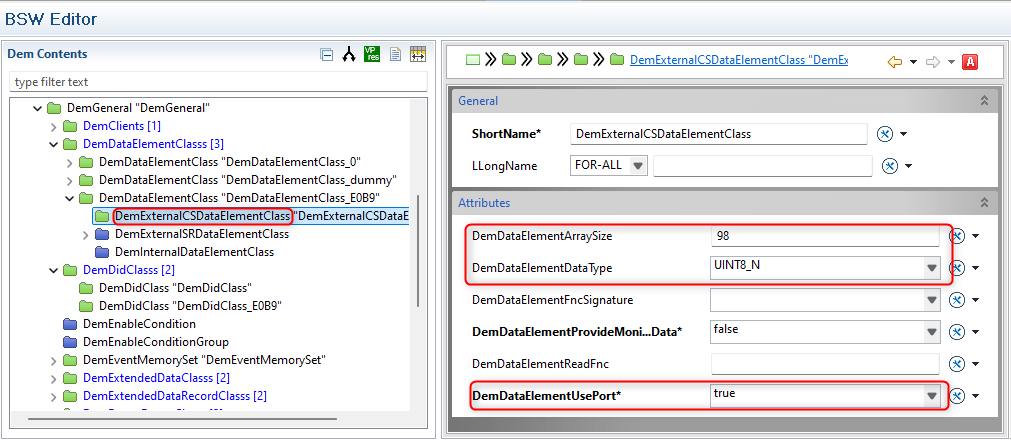
\includegraphics[scale=0.50]{images/dem_ff_87.png}
\end{figure}

and reference it in the related DemDidClass and DemExtendedDataRecordClass, link them to a DemFreezeFrameClass and this to a DemDTCAttributes. 
The DemDTCAttributes will be referenced in the DemDTC. 

From the SSFM side instead, the used must configure the reference 
\\ \textbf{Sum\_Ssfm\_DemDataElementClass\_XXXX87\_Ref} at least one Dem Event is configured in \\ Sum\_Ssfm\_GroupInfo subcontainers.
It shall be linked to the DemDataElementClass container of the configured DemExternalCSDataElementClass.

\begin{figure}[H]
	\centering
	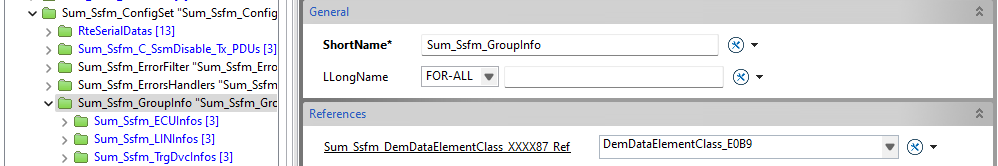
\includegraphics[scale=0.50]{images/xx87ref.png}
\end{figure}

\subsection{Adding Message DTC U19A3\_8A Freeze Frame}
\label{sec:19a38aff}
The Freeze Frame data for the DTC U19A3\_8A is provided by the SSFM module and it's the same content of the DID E0BB. 
If not automatically provided by the DEXT Arxml elaboration, the user must configure the Freeze Frame data in the Dem module, so mainly a DemExternalCSDataElementClass as in the picture:

\begin{figure}[H]
	\centering
	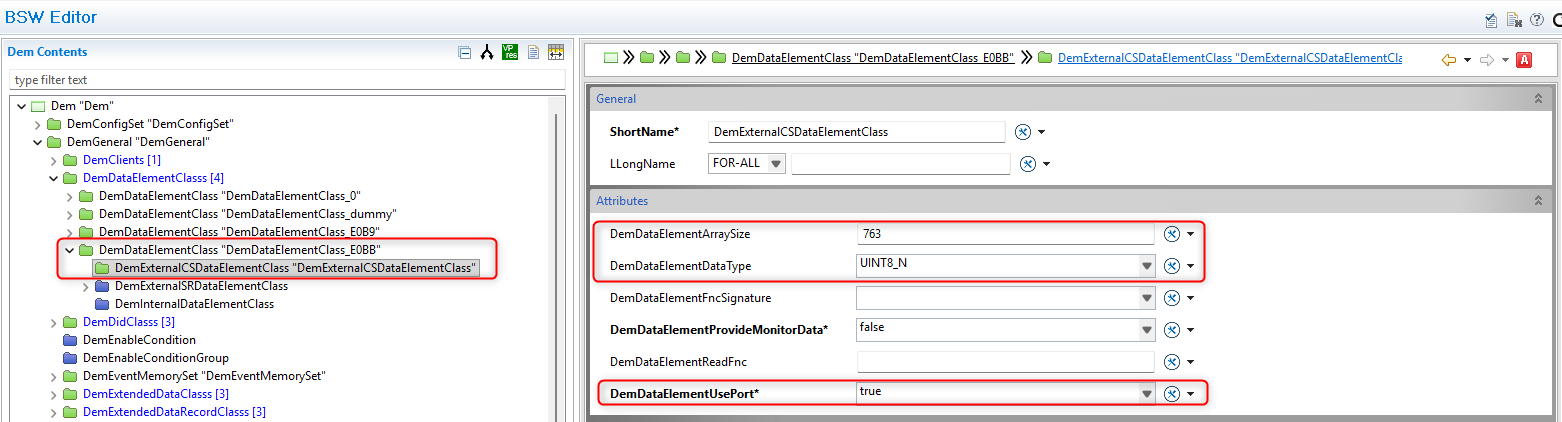
\includegraphics[scale=0.35]{images/dem_19a3_8a.png}
\end{figure}

and reference it in the related DemDidClass and DemExtendedDataRecordClass, link them to a DemFreezeFrameClass and this to a DemDTCAttributes. 
The DemDTCAttributes will be referenced in the DemDTC. 

From the SSFM side instead, the used must configure the reference 
\\ \textbf{Sum\_Ssfm\_DemDataElementClass\_U19A3\_8A\_Ref} at least one Dem Event is configured in \\ Sum\_Ssfm\_Errh\_KeySlotVerifyFilter subcontainers.
It shall be linked to the DemDataElementClass container of the configured DemExternalCSDataElementClass.

\begin{figure}[H]
	\centering
	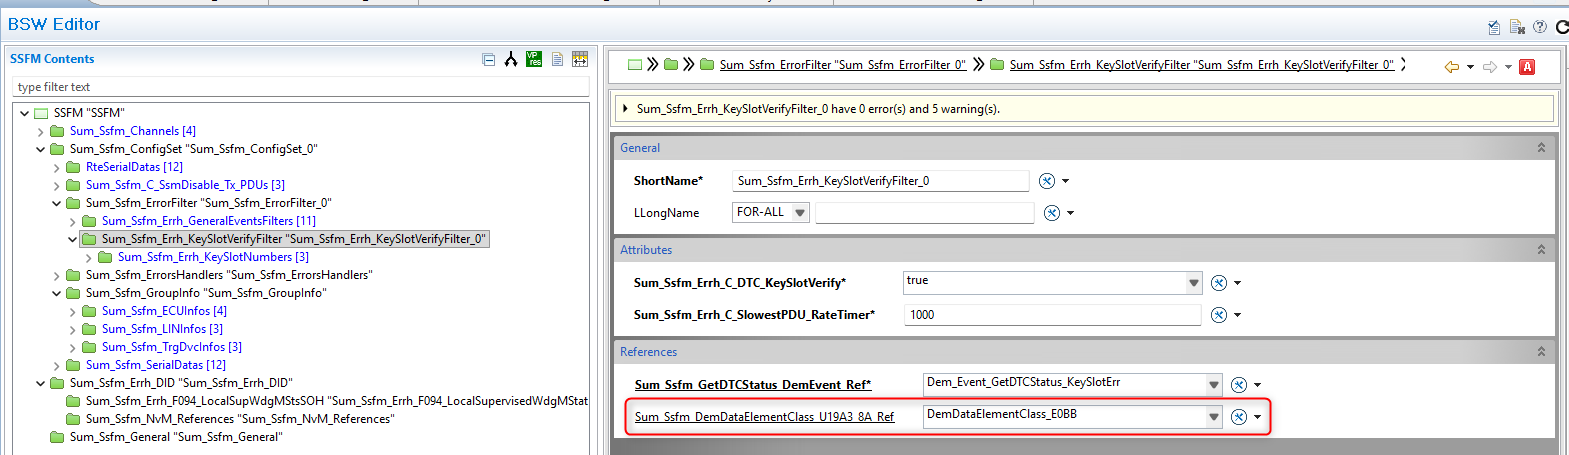
\includegraphics[scale=0.35]{images/19a3_8a_ref.png}
\end{figure}

\subsection{QoS Configuration for Consolidated Services}
\label{subsec:qosconfig}

The SSFM module provides support for Quality of Service (QoS) indication handling in consolidated service-based communication. This feature allows monitoring and dispatching of diagnostic QoS bytes (Availability, Lost Communication Fault Active, Failed Safety Indication, Failed Safety Fault Active) from host builds to satellite ECUs in MCU Farm architectures.

QoS support is currently available \textbf{only for service-based communication}. Signal-based communication is \textbf{not supported} because the System Extract ARXML does not currently provide QoS ImplementationDataType definitions for signals. All QoS-related configuration and generated artifacts apply exclusively to SerialDatas referencing service events (not signal groups).

\paragraph{Enabling QoS Support}
To enable QoS processing, the user must set the \texttt{SSFM\_QoS\_Enabled} parameter (located in \\ \texttt{Sum\_Ssfm\_General}) to \texttt{TRUE} (default value). When disabled, no QoS-related interfaces, ports, or code will be generated.

\paragraph{Data Type mapping}
In order to let Confgen generate accordingly the SomeIPXf, it is necessary to reference in the \\ \texttt{Sum\_Ssfm\_QoS\_DataTypeMappingSet} parameter (located in \texttt{Sum\_Ssfm\_General}) a DataTypeMappingSet containing the mapping between 
the Consolidated Service Payload APPLICATION-DATA-TYPE and the corresponding IMPLEMENTATION-DATA-TYPE.

\paragraph{Configuring QoS References}
For each service-based \texttt{Sum\_Ssfm\_SerialData} requiring QoS handling, the user shall configure one or more \texttt{Sum\_Ssfm\_QoS\_Ref} foreign references pointing to the QoS byte elements (IMPLEMENTATION-DATA-TYPE-ELEMENT) within the consolidated service payload structure. 
The code generator will:
\begin{itemize}
    \item Create a single R-Port to read the consolidated PDU payload
    \item Generate P-Ports for each configured \texttt{Sum\_Ssfm\_QoS\_Ref} 
    \item Generate an additional P-Port for the PDU-level QoS
\end{itemize}

\paragraph{Constraints}
The SSFM module assume the following: 

\begin{itemize}
    \item Each Consolidated Service SHALL be mapped to at most one \texttt{Sum\_Ssfm\_SerialData} 
	\item Each \texttt{Sum\_Ssfm\_Qos\_Ref} referenced in a \texttt{Sum\_Ssfm\_SerialData} SHALL belongs to the same Consolidated Service payload structure
\end{itemize}